\documentclass[a4paper, pdftex, notitlepage, parskip]{scrreprt}
%
\usepackage[ngerman]{babel}
\usepackage[T1]{fontenc}
\usepackage{lmodern}
\usepackage[latin1]{inputenc}
\usepackage[pdfborder={0 0 0}, pdfpagelabels={false}, bookmarksnumbered={true}, pdfcreator={}, pdfproducer={}]{hyperref}
\usepackage{rotating}
\usepackage[table]{xcolor}
\usepackage{tabularx}
\usepackage{fancyvrb}
\usepackage{amsmath}
\usepackage{enumerate}
%
\begin{document}
\title{\vspace{2cm} \Huge GhostDB - Ein Beispiel \vspace{2cm}}
\author{Martin Minor, David Sander}
\date{\today}
\maketitle
\vspace{2cm}
%
Dieses Beispiel soll die verwendeten Strukturen und Abl�ufe in dem System ``GhostDB'' verdeutlichen.
%
\tableofcontents
\listoffigures
\listoftables
\pagestyle{headings}
%
\chapter{Einf�hrung}

In der Vorlesung Techniken und Konzepte zum Schutz der Privatsph�re haben wir uns mit verschiedenen Techniken und Verfahren zur Anonymisierung von sensitiven Daten und deren Sicherung besch�ftigt. Eine hierbei behandelte Idee ist die sogenannte ``GhostDB''.\footnote{GhostDB: Hiding Data from Prying Eyes} \footnote{GhostDB: Querying Visible and Hidden Data Without Leaks} \footnote{Vortrag: GhostDB: Hiding Data from Prying Eyes (Technology)}

Das gesamte System, welches die ``GhostDB'' umfasst basiert auf verschiedenen Komponenten und ist sehr umfangreich. Wir beschr�nken uns daher in dieser Arbeit auf das sogenannte Post- und Prefiltering. Beide Verfahren werden bei der Abarbeitung von Anfragen eingesetzt um diese m�glichst effizient und schnell zu beantworten. Wir werden diese Techniken kurz vorstellen und anhand eines kleinen Beispieles ihre Funktionsweise erkl�ren.

Im folgenden wollen wir eine kurze Einf�hrung in unsere Datenbasis geben um sp�ter auf diese zur�ckgreifen zu k�nnen.	
	
\chapter{Datenbasis}

In den Papern zu diesem Thema wurden meist Beispiele aus dem medizinischen Bereich gew�hlt mit �rzten, Patienten, Untersuchungen etc. Wir haben uns nach reiflicher �berlegung f�r den Bereich des Flugverkehrs entschieden. In diesem Feld existieren viele verschiedene Daten, die je nach Angreifermodell und Nutzer zu sch�tzen sind. Eine Fluggesellschaft ist zum Beispiel daran interessiert, welche Reisende ihr Kontigent an Gep�ckst�ckem beziehungsweise mitzuf�hrendes Gep�ckgewicht �berschreiten, um ihnen beim n�chsten Flug ein teureres Ticket verkaufen zu k�nnen. Auf die Spitze getrieben m�chte ein Terrorist in Erfahrung bringen, welcher Pilot ein bestimmtes Flugzeug fliegt und ob bestimmte Personen, wie zum Beispiel Polizisten, im Flugzeug sitzen.

Die Herausforderung bestand erst einmal in der Suche nach dem aus unserer Sicht besten Datenmodell f�r dieses Szenario, welches nicht zu komplex ausf�llt um den Rahmen dieser Arbeit nicht zu sprengen. Ein weiterer Augenmerk lag darauf, so wenig Daten wie m�glich in den ``sicheren'' Bereich der sp�teren ``GhostDB'' zu verlagern ohne die Sicherheit der Daten zu gef�hrden.\textbf{(TODO: noch mal durchlesen, gef�llt mir noch nicht von der Formulierung)}.

\begin{figure}[htb]
  \centering%
  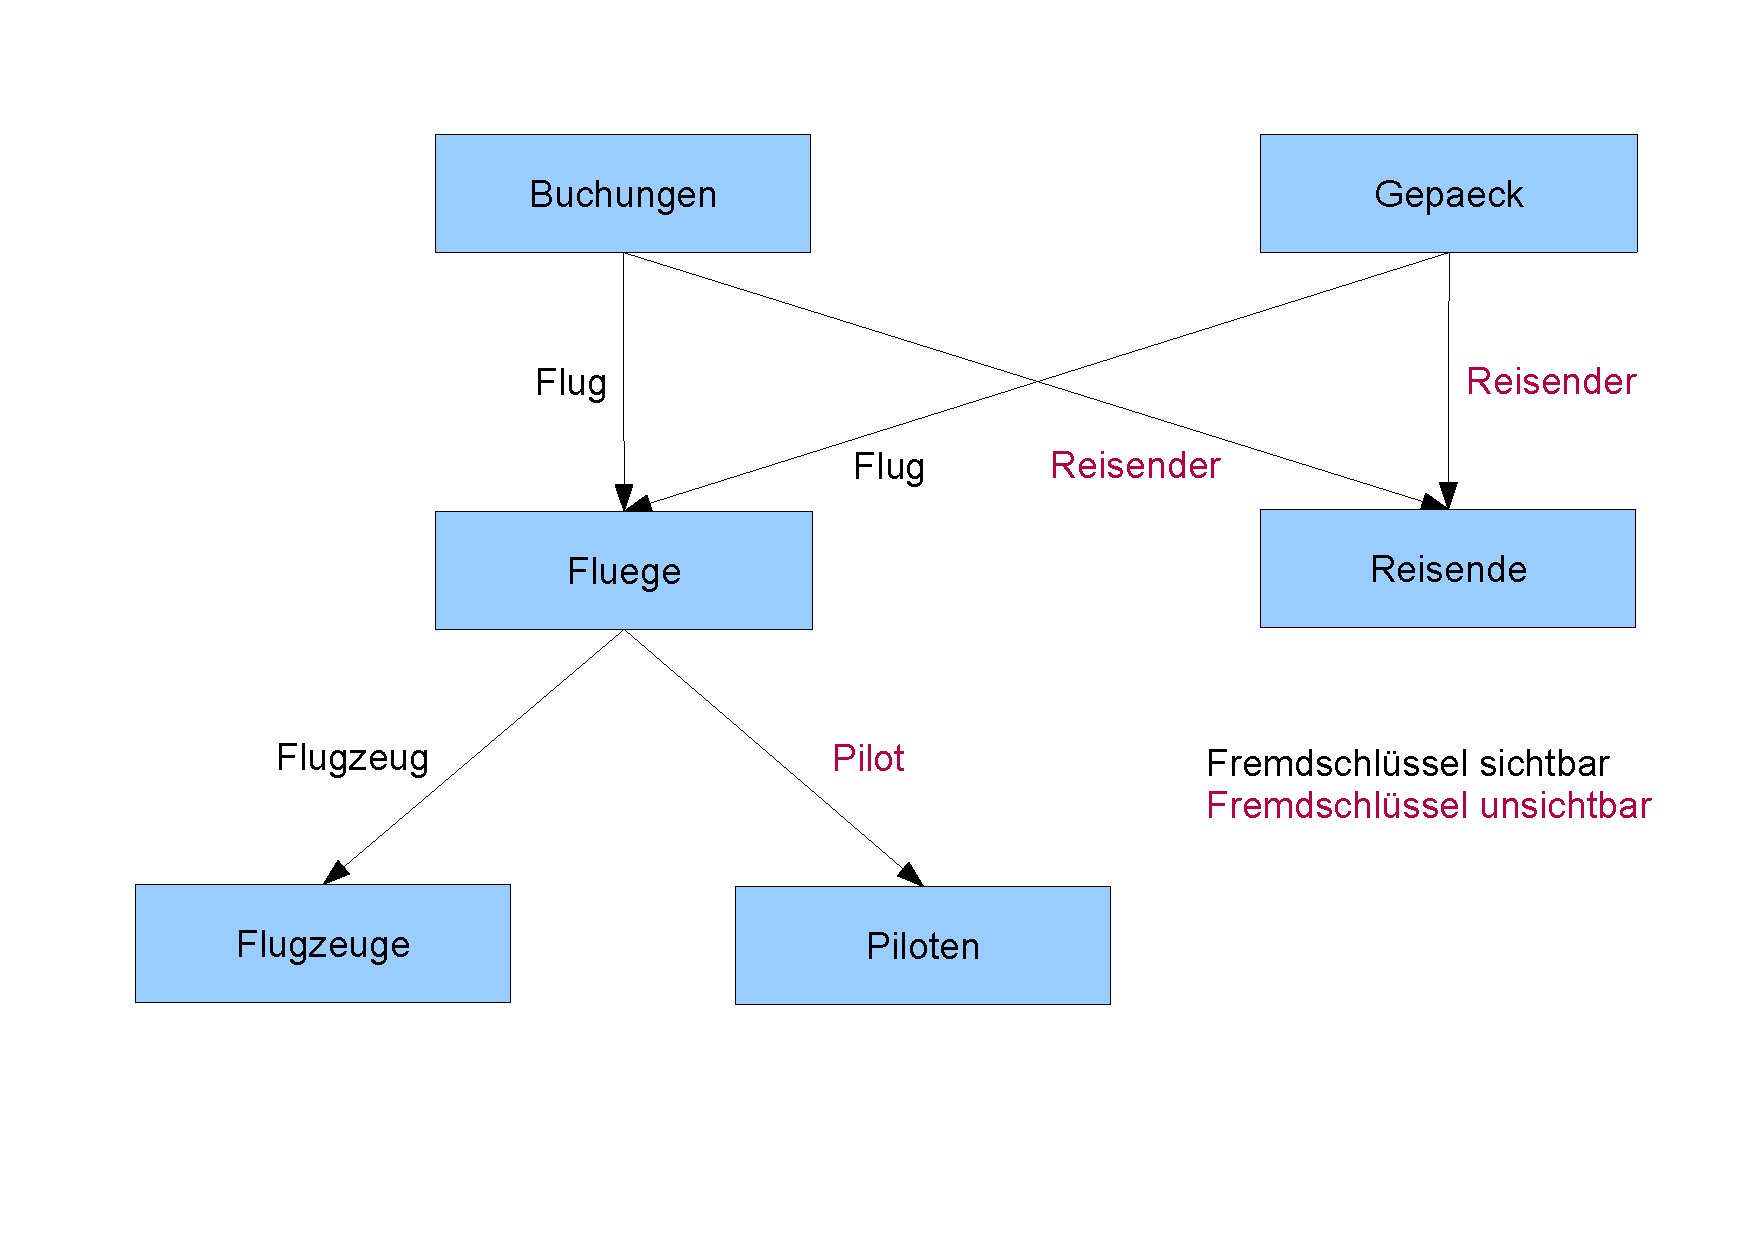
\includegraphics[width=0.8\linewidth]{img/Datenmodell.pdf}%
  \caption{Datenmodell}
  \label{fig:Datenmodell}
\end{figure}%

\chapter{Datenstrukturen TODO: bessere Erkl�rung}

Um im Laufe der Erkl�rungen zu den verschiedenen Methoden einen Ablaufplan f�r eine Anfrage auf der ``GhostDB'' zu erstellen werden verschiedenen Datenstrukturen ben�tigt. Einige von ihnen wollen wir kurz vorstellen.

\section{Subtree Key Table}

Eine dieser Strukturen ist der ``Subtree Key Table''. Hierbei enth�lt die Wurzeltabelle  alle ID's der nachfolgenden Tabellen, ??? \textbf{TODO: SKT und CI beschreiben}

\section{Climbing Index}

Eine weitere Struktur ist der ``Climbing Index''......

\chapter{Warum Filter ?}

Das System ``GhostDB'' hat das Problem, dass alle Berechnungen die Bezug auf die unsichtbaren Daten auf dem ``SmartUSB''-Stick nehmen in diesem berechnet werden m�ssen. Da der Speicher f�r die Ausf�hrung auf diesem Ger�t aber begrenzt ist, entsteht hier ein Ressourcenproblem, da alle Daten in den Speicher geladen werden m�ssen und weiterhin in diesem auch Platz f�r das Ergebnis vorhanden sein muss. Die Autoren der Paper haben daher eine M�glichkeit gesucht die Menge an Informationen, die in den Speicher geladen werden m�ssen, um eine Antwort auf die gestellte Anfrage zu erhalten, zu verringern. Das Ergebnis waren die Post-, Pre- und Crossfilter. In dieser Arbeit werden wir nur auf die ersten beiden eingehen.

\section{Prefiltering}

Die Idee beim Prefiltering ist, dass alle Selektionen zuerst ausgef�hrt werden um die gesamte Datenmenge die bei Joins und Mergeoperationen verwendet werden so gering wie m�glich zu halten. Weiterhin wird versucht so viele Selektionen wie m�glich auf dem unsicheren Bereich auszuf�hren, da die Ressourcen hier nicht so beschr�nkt sind, wie im sicheren Bereich. Selektionen auf Daten die den sicheren Teil der ``GhostDB'' betreffen k�nnen allerdings auch nur in diesem ausgef�hrt werden. F�r die Selektionen werden nach M�glichkeit ``Climbing'' Indizes verwendet. Die danach folgenden Joins werden dann im sicheren Bereich ausgef�hrt, hierbei wird dann meist ein ``Subtree Key Table'' verwendet.

\section{Postfiltering}

Beim Postfiltering wird ein anderes Verfahren verwendet. Es wird hier zuerst der Join auf dem sicheren Teil der ``GhostDB'' ausgef�hrt. Im folgenden werden die m�glichen Selektionen des unsicheren Bereiches zu den erzeugten Ergebnissen hinzugef�gt. Dies geschieht entweder durch das Erzeugen eines Blommfilters aus diesen Daten, der dann f�r die Filterung der bisherigen Ergebnisse benutzt wird oder genau umgekehrt. Im umgedrehten Fall wird der Bloomfilter aus den vorhandenen Resultaten gebildet und die Daten der Selektion werden mit diesem gefiltert. Die �brig gebliebenen Daten werden dann weiterverabeitet. \textbf{TODO: hier k�nnte noch mehr kommen}

Cross-Filtering kann teilweise bessere Ergebnisse erzielen. Es wird versucht die Kardinalit�t von Zwischenergebnissen des unsicheren Ger�ts so klein wie m�glich zu halten, indem ``Filter'' oder ``Merge''-Operationen mit sicheren Daten so fr�h wie m�glich durchgef�hrt werden.

\chapter{Anwendung}

Die folgenden Beispiele zum Pre- und Postfiltering basieren auf der oben schon vorgestellten Datenbasis und der folgenden Anfrage:


\begin{Verbatim}[commandchars=\\\{\}]
SELECT R.ReisenderID, R.Vorname, R.Name, R.Staatsbuergerschaft
FROM Buchungen B, Gepaeck G, Fluege F, Reisende R, Piloten P
WHERE R.Geschlecht='M' AND P.Geburtsdatum<1956-08-01 AND G.Gewicht>20
    AND B.Flug=F.FlugID AND B.Reisender=R.ReisenderID
    AND G.Flug=F.FlugID AND G.Reisender=R.ReisenderID
    AND F.Pilot=P.PilotID
\end{Verbatim}

Die genauen Funktionsaufrufe, die in den Papern erkl�rt sind, sind unter dem Abschnitt Query Execution Plan zu finden. Die Funktionsweise der einzelnen Funktionen (bis auf MJoin, dass leider nie deklariert oder definiert wurde) kann in den entsprechenden Papern nachgelesen werden.

\section{Prefiltering}

Beim Prefiltering-Verfahren kommt es wie oben schon erw�hnt darauf an die Selektionen der Anfrage (Query) \textbf{TODO: Was ist besser Query und Anfrage verwenden oder jeweils nur eines der beiden W�rter???} so fr�h wie m�glich auszuf�hren um weniger Daten f�r die weitere Verarbeitung zu haben. In unserem Beispiel kommen drei Selektionen vor. Diese sind die Auswahl des Geschlechts des Reisenden, das Geburtsdatum des Piloten und das Gewicht des Gep�cks. In der Regel ist eine Selektion immer dann am schnellsten, wenn Sie einen Bereich betrifft der nicht versteckt ist, da hier alle Ressourcen der unsicheren Plattform genutzt werden k�nnen. Diese sind meist um ein vielfaches h�her als die des ``SmartUSB''-Sticks. Aus diesem Grund beginnen wir mit der Auswahl des Gewichts. Wir wollen alle GepaeckIds herausfiltern f�r die gilt, dass das ihnen zugeordnetes Gewicht gr��er als 20 Kilogramm ist. Dies w�ren die folgenden IDs (siehe Tabelle \ref{tab:Gepaeck}):  G06, G12, G13, G16, G18, G19, G20, G22, G23.
 \textbf{TODO: hier sollte irgendwie erw�hnt werden das die GIds zur sicheren Plattform �bertragen werden}
\\ 
Der n�chste naheliegende Schritt w�re die Auswahl des Geschlechts der Reisenden, da diese Eigenschaft nicht versteckt ist. Aus Gr�nden die sp�ter noch erl�utert werden ignorieren wir diese Selektion erst einmal. 
Es bleibt demzufolge nur noch die Selektion auf den Geburtsdaten der Piloten �brig. Diese Eigenschaft ist versteckt und muss daher auf der sicheren Plattform ausgef�hrt werden. Als Ergebnis w�rden wir alle PilotIds erhalten, deren Geburtstag vor dem 01.08.1956 liegt. Mit dieser Information kann aber nur schlecht weitergearbeitet werden, da bis jetzt nur GepaeckIds vorliegen. Aus diesem Grund wird ein ``ClimbingIndex'' auf dem Attribut Geburtsdatum verwendet (siehe Tabelle \ref{tab:ClimbingIndexPilotenGeburtsdatum}) und auf diesem wird dann die Selektion ausgef�hrt. Als Ergebnis werden folgende GepaeckIds im sicheren Bereich vorgehalten: G07, G18, G19, G20, G25.

Die nun vorhandenen GepaeckIds k�nnen mittels der Schnittmenge verringert werden um den Aufwand f�r den nachfolgenden Join \textbf{TODO: darf man hier Join erw�hnen oder sollte es SJoin hei�en} zu verringern. Als Resultat erh�lt man: G18, G19, G20.

\begin{figure}[htbp]%
  \centering%
  \frame{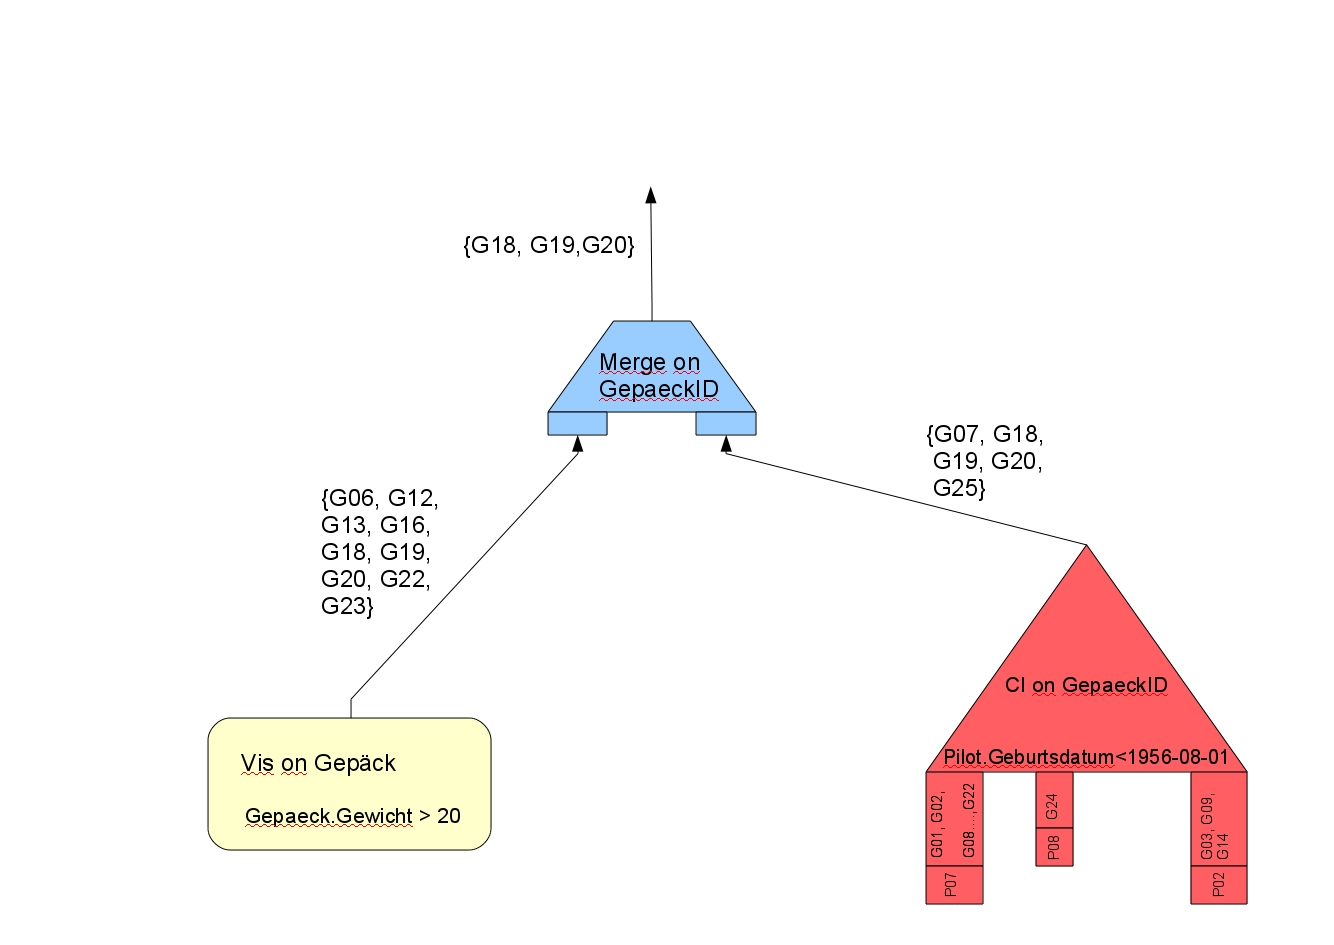
\includegraphics[width=1\linewidth]{img/Pre1}}
  \caption{Teilergebnis Pre-Filtering 1}%
  \label{fig:pre1}%
\end{figure}%

Im Nachfolgenden m�ssen alle ``Statements'' in der ``WHERE-Clause'' erf�llt werden. Dies geschieht unter zu Hilfenahme von Semi-Joins und diese werden wiederum durch ``Subtree Key Tables'' (SKT) unterst�tzt. Die ``WHERE-Clause'', die wir berechnen wollen ist folgende: G.Reisender=R.ReisenderID. Im SKT f�r Gepaeck (Tabelle \ref{tab:SKTGepaeck}) werden nun die ReisendenIDs zu den entsprechenden GepaeckIDs herausgesucht und mit dem SJoin zusammengef�hrt.\textbf{TODO: kann man das so schreiben ??}

Da wir nun ReisendeIDs haben kann die n�chste Bedingung in Angriff genommen werden: B.Reisender=R.ReisenderID. Hierf�r werden ReisendeIDs auf Basis der BuchungsIDs ben�tigt. Die Selektion mittels Gep�ckIDs entf�llt da diese keine direkte Verbindung zu den Buchungen haben. Da wir schon die Piloten vorhin als selektives Mittel verwendet haben tun wir dies noch einamal mittels eines ``Climbing Index'' auf den BuchungsIDs. Der ``Climbing Index'' liefert uns als Resultat eine Liste von Listen. Diese k�nnen wir f�r den SKT aber nicht verwenden, da dieser nur eine Liste als Eingabe akzeptiert. Die Die L�sung ist das Zusammenf�hren der einzelnen Liste zu einer Liste mit der Operation Vereinigung. Als Ergebnis wird folgendes geliefert: B08, B11, B18, B19, B20, B21.

\begin{figure}[htbp]%
  \centering%
  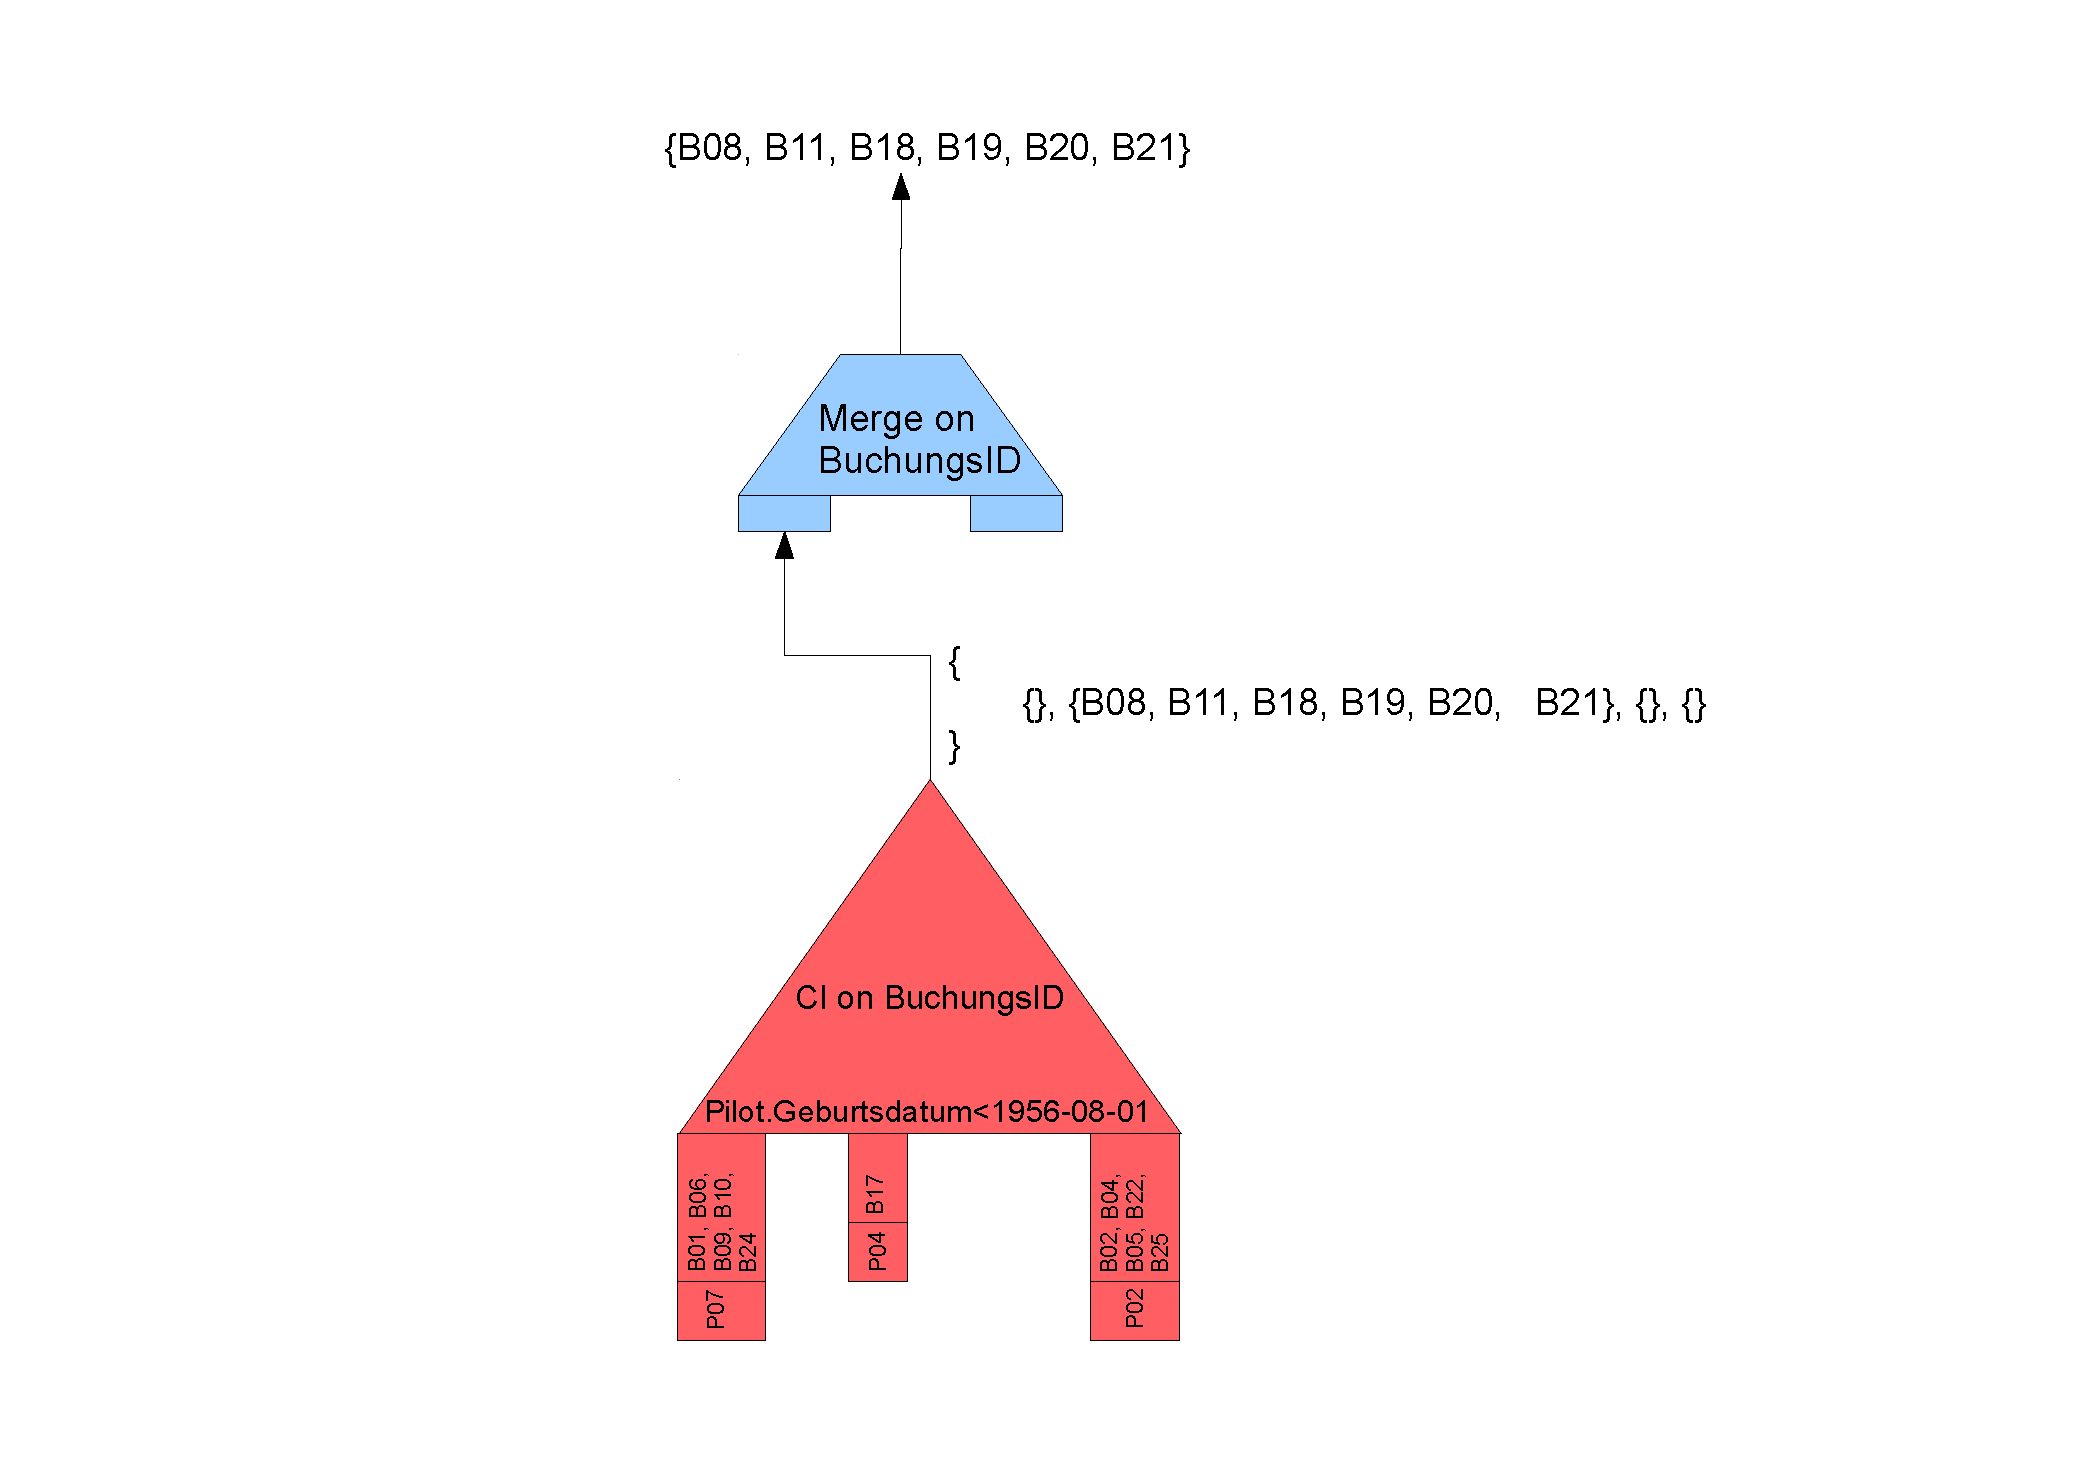
\includegraphics[width=1\linewidth]{img/Pre2.pdf}%
  \caption{Teilergebnis Pre-Filtering 2}%
  \label{fig:pre2}%
\end{figure}%

Die so erhaltenen BuchungsIDs werden analog zu den GepaeckIDs im vorherigen Schritt benutzt um ReisendeIDs zu berechnen. Um beide Bedingungen zu erf�llen muss nun noch der Durchschnitt der beiden ReisendeIDs durchgef�hrt werden. Damit w�ren beide Bedingungen erf�llt. Mit diesem Resultat kann dann weiter gearbeitet werden.

\begin{figure}[htbp]%
  \centering%
  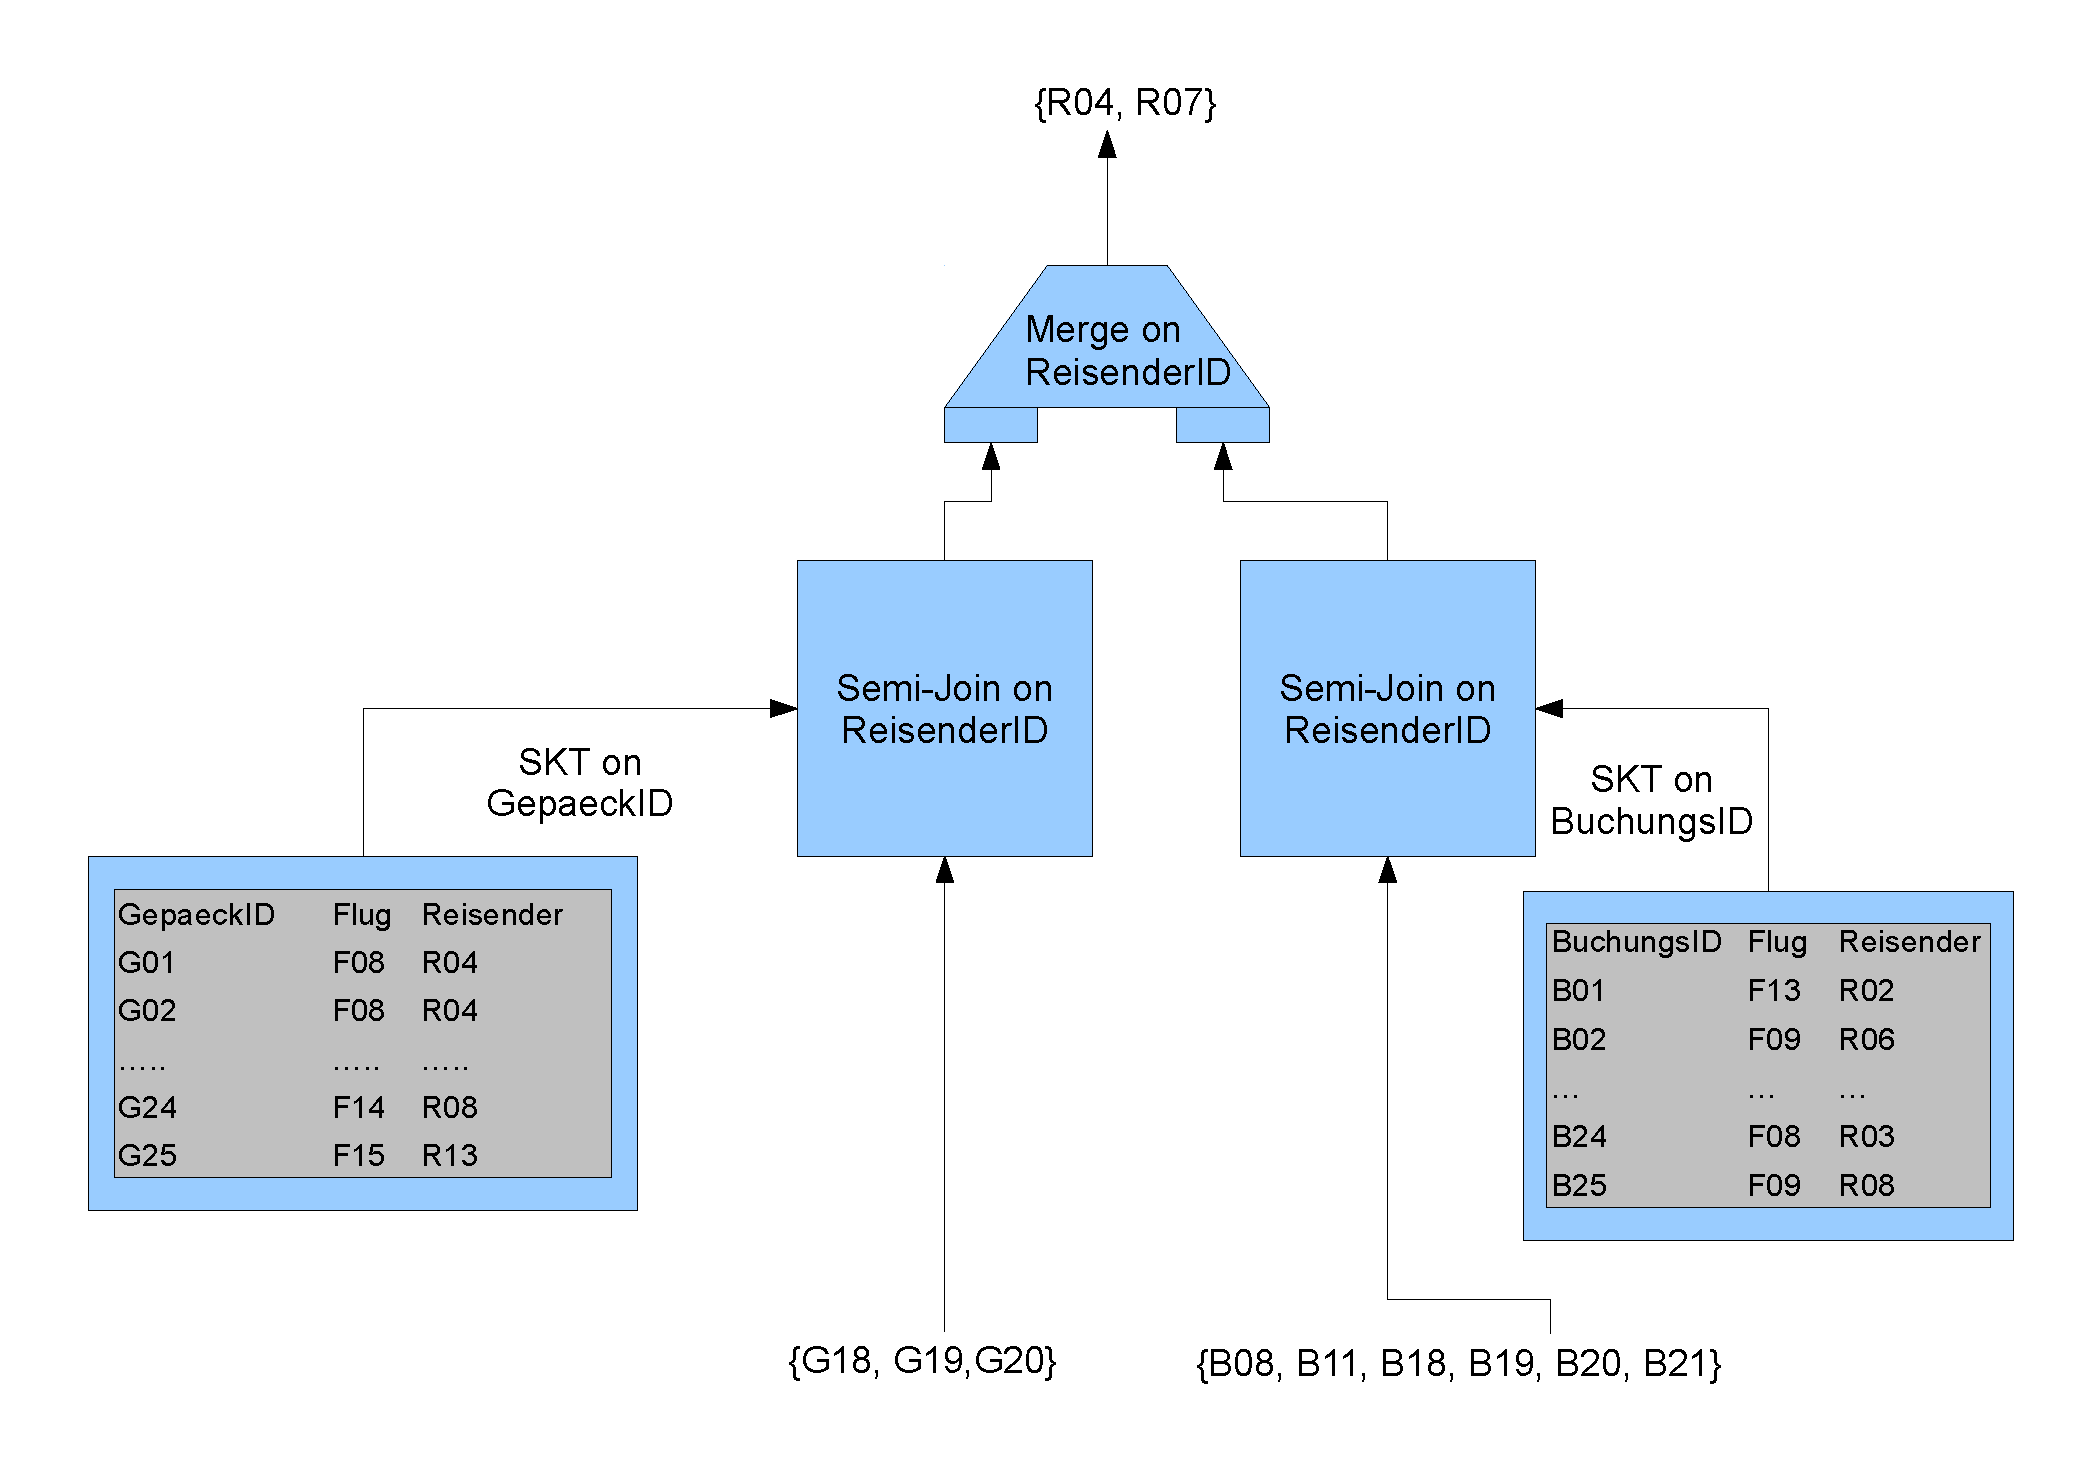
\includegraphics[width=1\linewidth]{img/Pre3.pdf}%
  \caption{Teilergebnis Pre-Filtering 3}%
  \label{fig:pre3}%
\end{figure}%

Auf dieser entstandenen Datenbasis wird nun ein Bloomfilter gebaut, der f�r die noch nicht angewandte Selektion verwendet wird. Die fehlende Selektion ist: R.Geschlecht='M'. Die Selektion wird erst jetzt angewandt, da sie sonst vorher in den beiden Joins die zu bearbeitenden Datenmengen erh�ht h�tte. Durch den sp�teren Einsatz k�nnen die Datenmengen geringer gehalten werden und der Rechenaufwand ist somit geringer.

\begin{figure}[htbp]%
  \centering%
  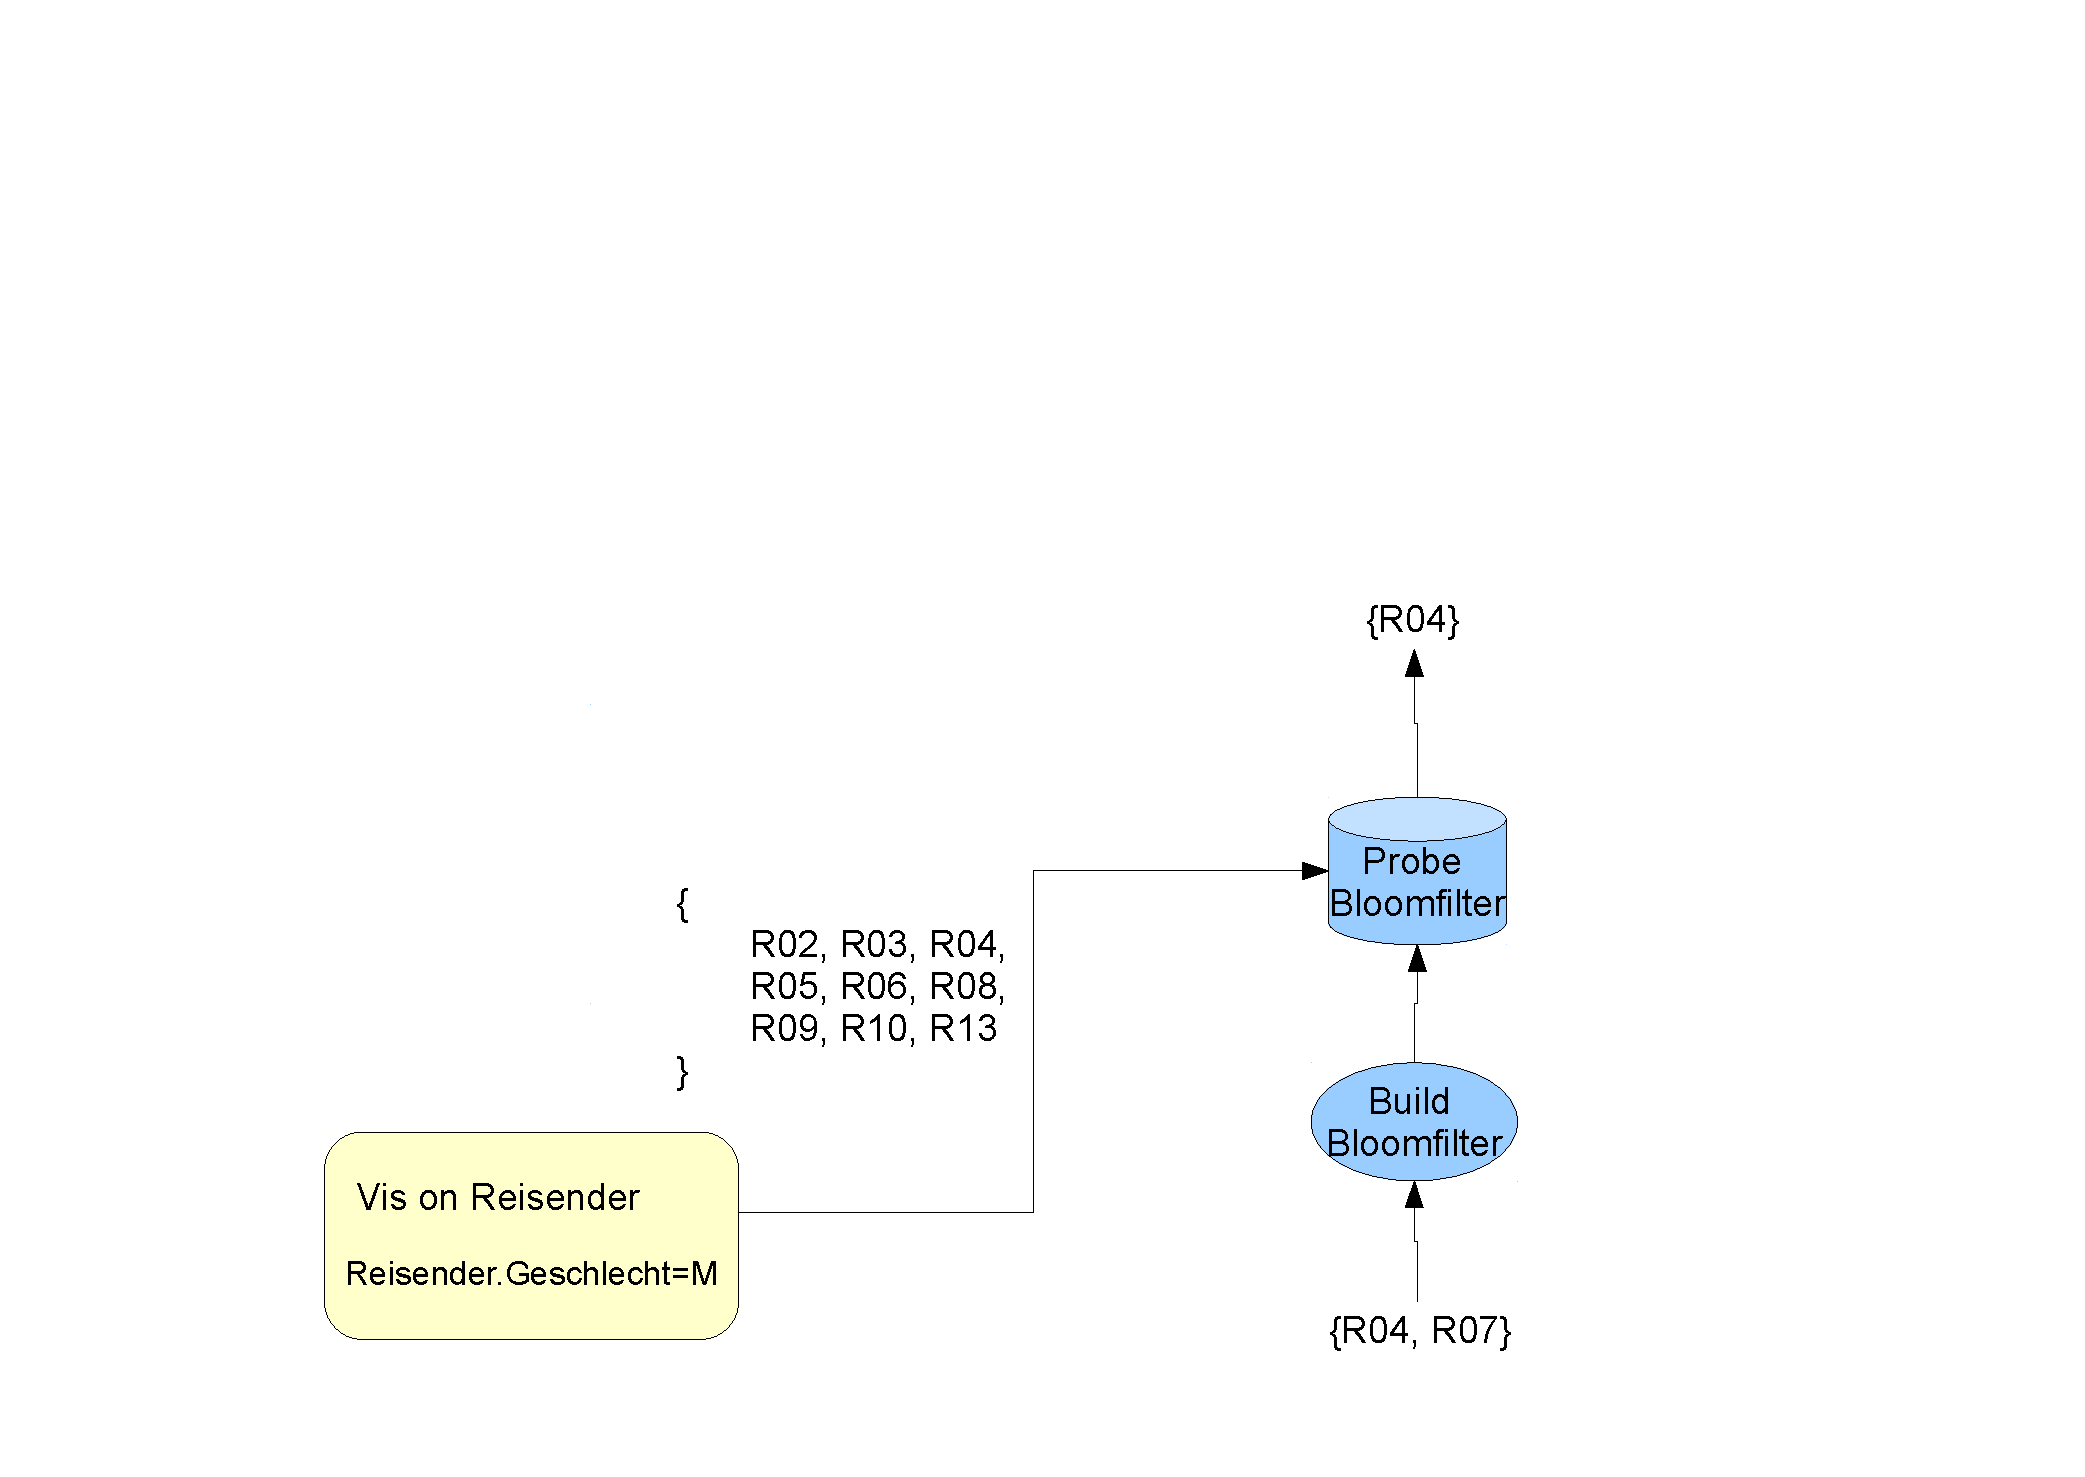
\includegraphics[width=1\textwidth]{img/Pre4.pdf}%
  \caption{Teilergebnis Pre-Filtering 4}%
  \label{fig:pre4}%
\end{figure}%

Als Abschluss m�ssen nur noch die entsprechenden Projektionen angewendet werden. Dies geschieht mittels eines MJoins. Dieser ben�tigt aber nochmals alle ReisendeIDs mit der Eigenschaft das das Geschlecht m�nnlich ist. Bei dieser Anfrage werden aber nicht nur die ReisendeIDs ben�tigt, sondern auch die Attribute f�r Vorname und Name. Als Ergebnis kann dann folgendes ausgegeben werden: \{$\langle$R04,Doru,Davidovici,Rom�nisch$\rangle$\}.

\begin{figure}[H]%
  \centering%
  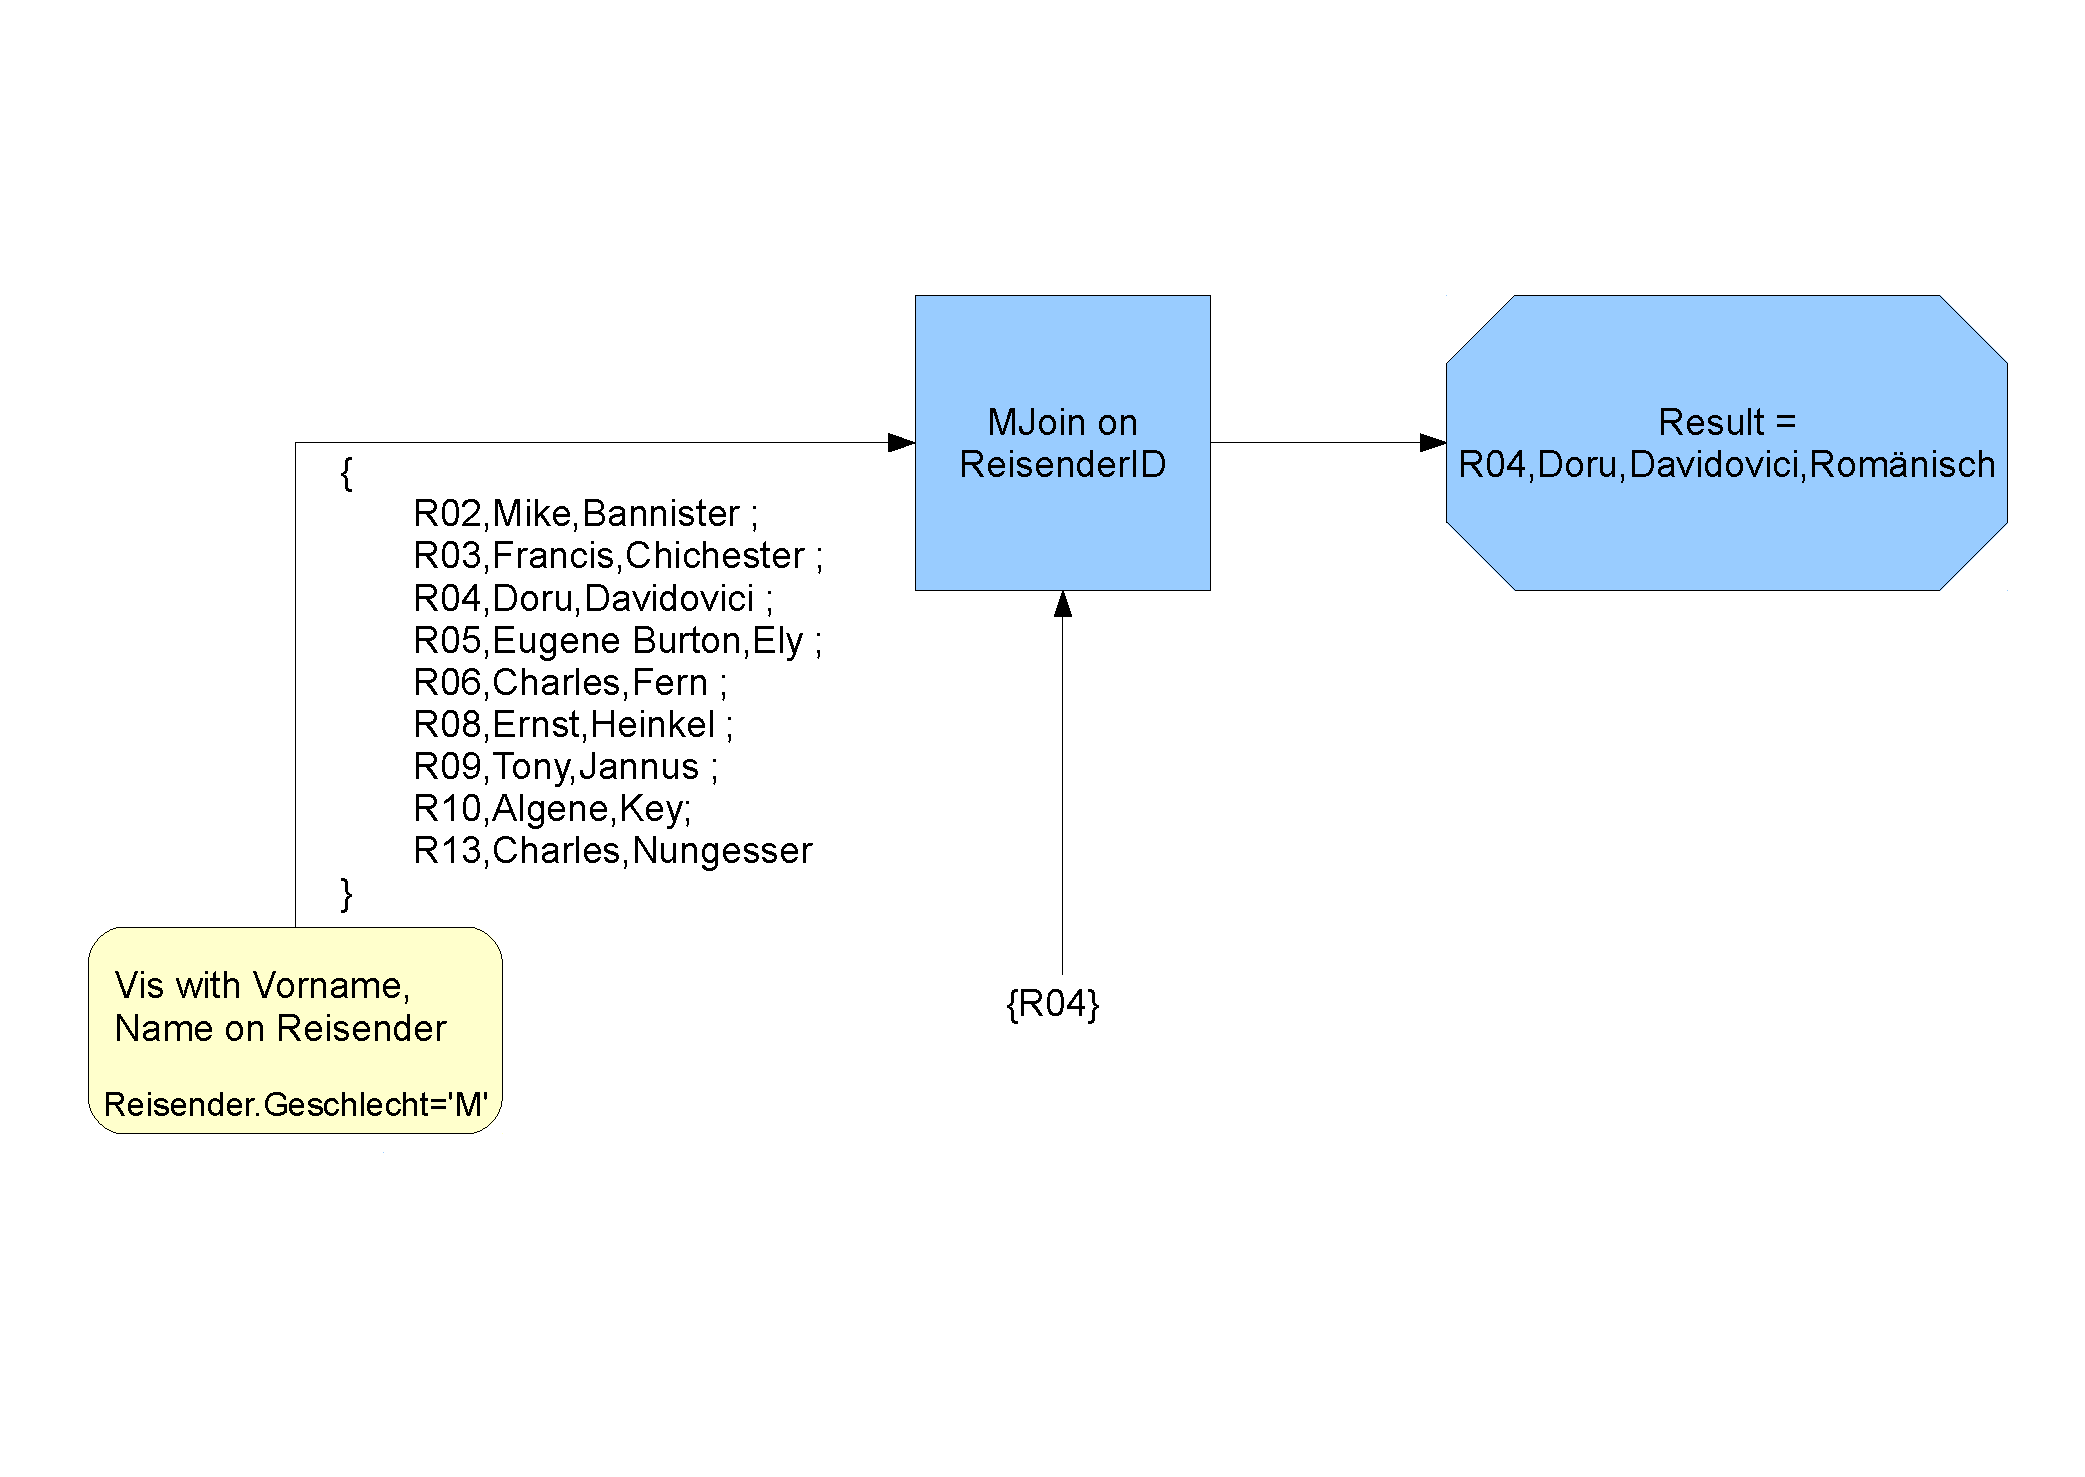
\includegraphics[width=1\textwidth]{img/Pre5.pdf}%
  \caption{Teilergebnis Pre-Filtering 5}%
  \label{fig:pre5}%
\end{figure}%

F�gt man die einzelnen Schritte zusammen entsteht folgender Ausf�hrungsplan f�r das Prefiltering:


\begin{figure}[H]%
  \centering%
  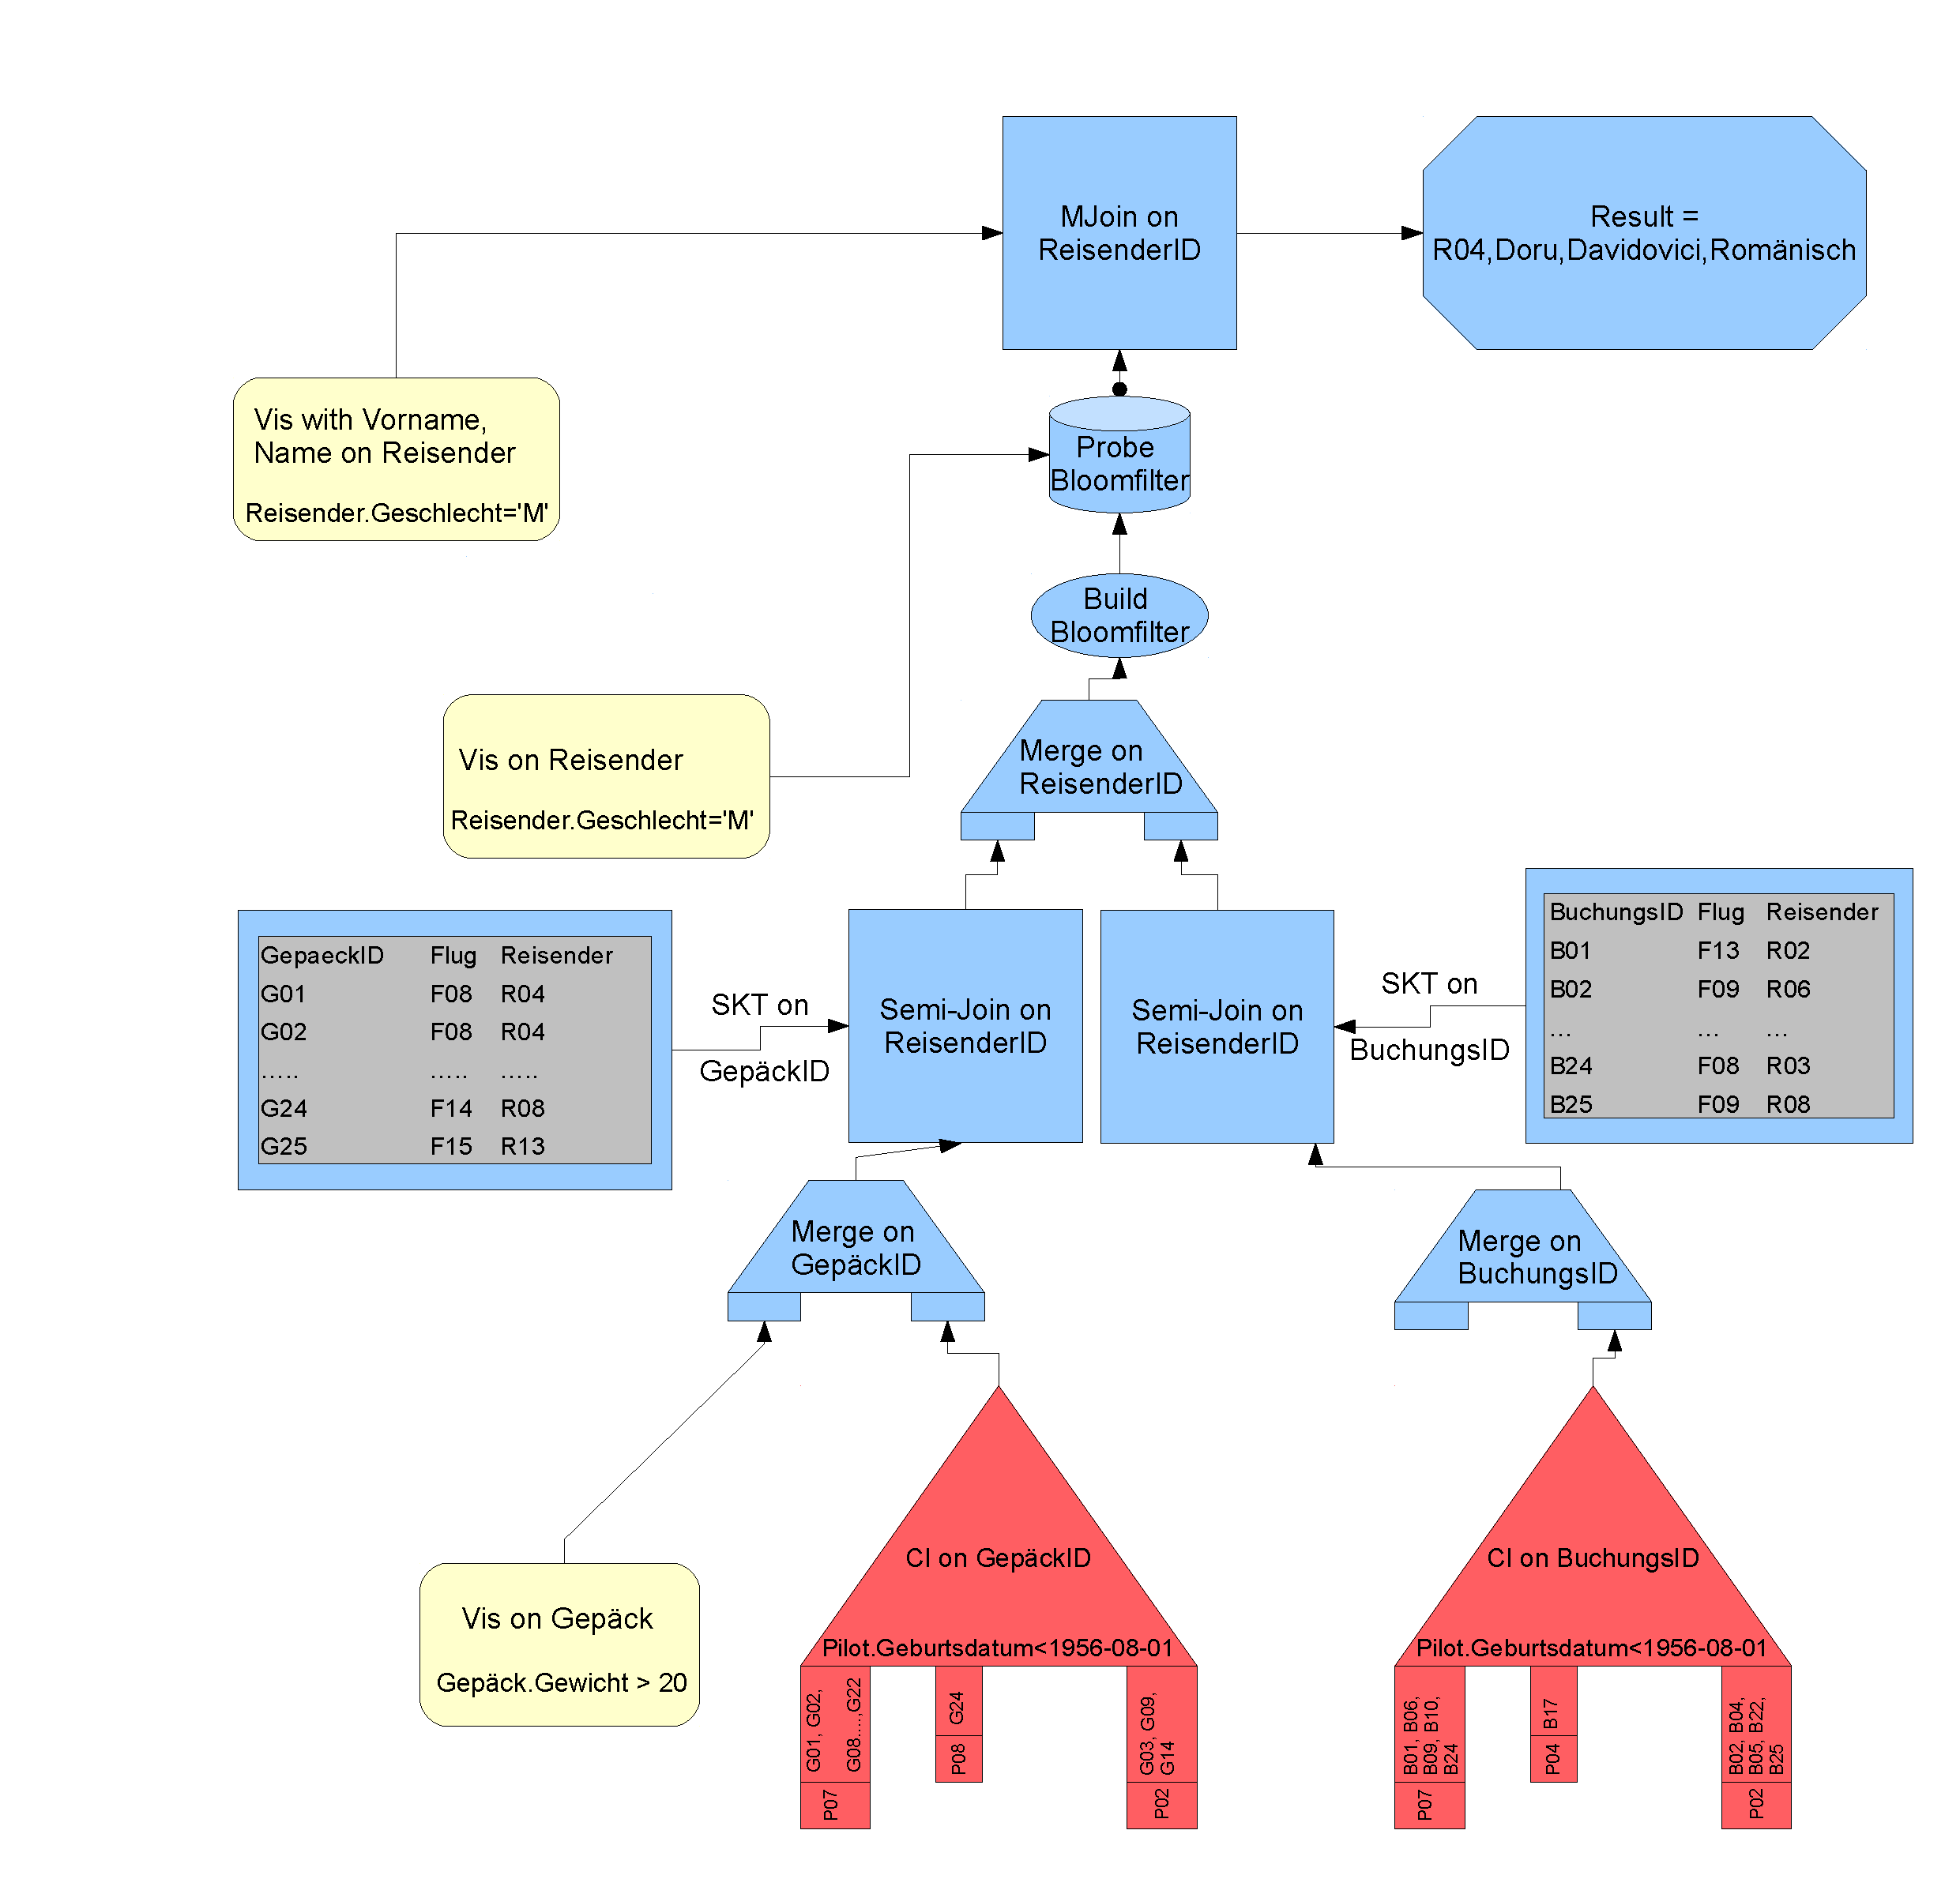
\includegraphics[width=1\textwidth]{img/Pre-Filtering.pdf}%
  \caption{Pre-Filtering QEP}%
  \label{fig:pre}%
\end{figure}%

Die einzelnen ``Methoden'' die zur Berechnung verwendet wurden kann man sich unter Kapitel ~\ref{chp:Query Execution Plans} noch einmal genauer ansehen. Auf den ersten Blick scheint die L�sung des Prefilterings optimal zu sein, da man schon im Vorfeld viele Daten \textbf{TODO: ist Daten das Richtige Wort ???} aus der Berechnung der Joins herausnehmen kann und somit den Aufwand verringert.

Das Problem an dieser Strategie ist allerdings, dass bei zu geringer Selektivit�t Selektionen zu wenige Tupel im Vorfeld aussortiert werden und somit ein gro�er Vorteil des Prefilterings verschwindet. Eine andere Alternative, die dem eben angesprochenen Effekt nicht so stark unterliegt ist das Postfiltering.

\section{Postfiltering}

Beim Postfiltering werden zuerst alle Selektionen ausgef�hrt und per Join zusammengefasst, die auf den sicheren Bereich zugreifen. Erst danach werden mittels ``Fuzzy filtering''\footnote{GhostDB: Hiding Data from Prying Eyes(Technology) Vortrag} die Selektionen des unsicheren Bereiches hinzugef�gt.

F�r unser Beispiel hei�t dies, dass zuerst die Selektion auf dem Geburtsdatum des Piloten ausgef�hrt wird. Da wir mit der PilotID aber nicht ohne Weiteres weiterarbeiten k�nnen, verwenden wir hierf�r den ``Climbing Index'' auf der GepaeckID und f�hren auf diesem Ergebnis eine Vereinigung aus, da wir nur eine Liste von GepaeckIDs gebrauchen k�nnen.

\textbf{TODO: bessere Skalierung f�r das Bild w�hlen}
\begin{figure}[htbp]
  \centering
  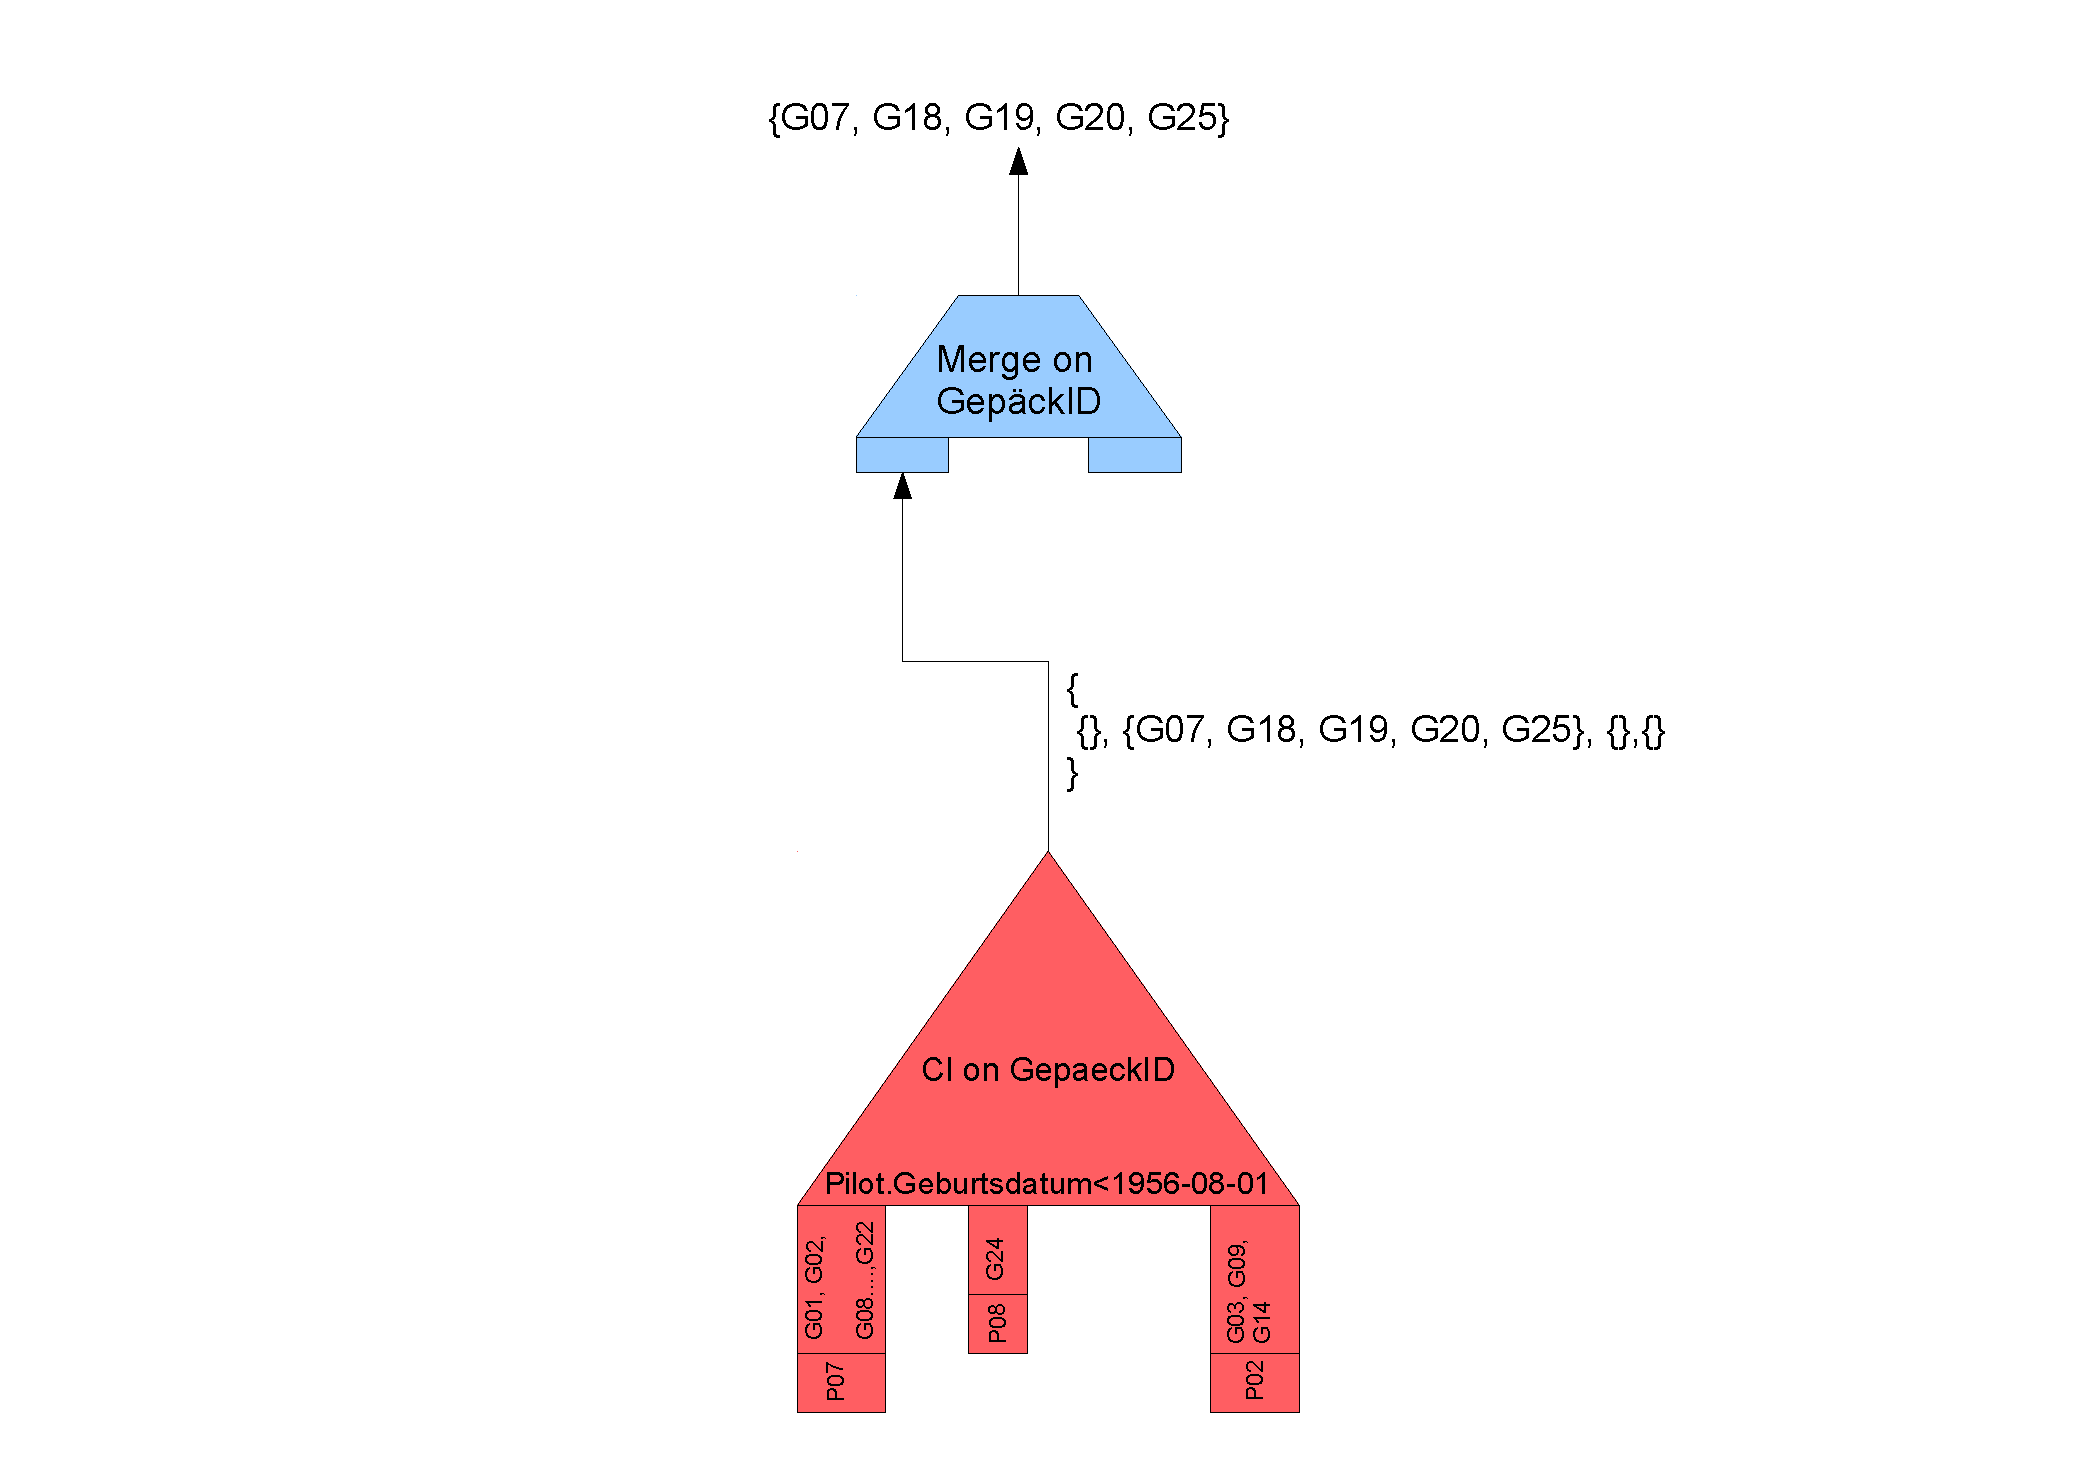
\includegraphics[width=1\textwidth]{img/Post1.pdf}
  \caption{Teilergebnis Post-Filtering 1}
  \label{fig:post1}
\end{figure}

Diese Selektion ist in unserem Beispiel die Einzige die auf den unsicheren Bereich zugreift, nach dem Verfahren des Postfilterings werden diese IDs nun f�r einen Join benutzt. Als Ergebnis brauchen wir wiederum ReisendeIDs, da diese f�r die sp�tere Projektion notwendig sind. Um diese IDs zu erhalten bedienen wir uns wieder dem ``Subtree Key Table'' und Filtern uns somit alle ReisendeIds heraus. Bei den Selektionen aus dem unsicheren Berich erhalten wir aber GepaeckIds, daher gibt uns der Join auf unsere Anforderung hin eine Menge von Tupeln aus GepaeckID und dazu passender ReisenderID heraus.

\textbf{TODO: bessere Skalierung f�r das Bild w�hlen}
\begin{figure}[htbp]
  \centering
  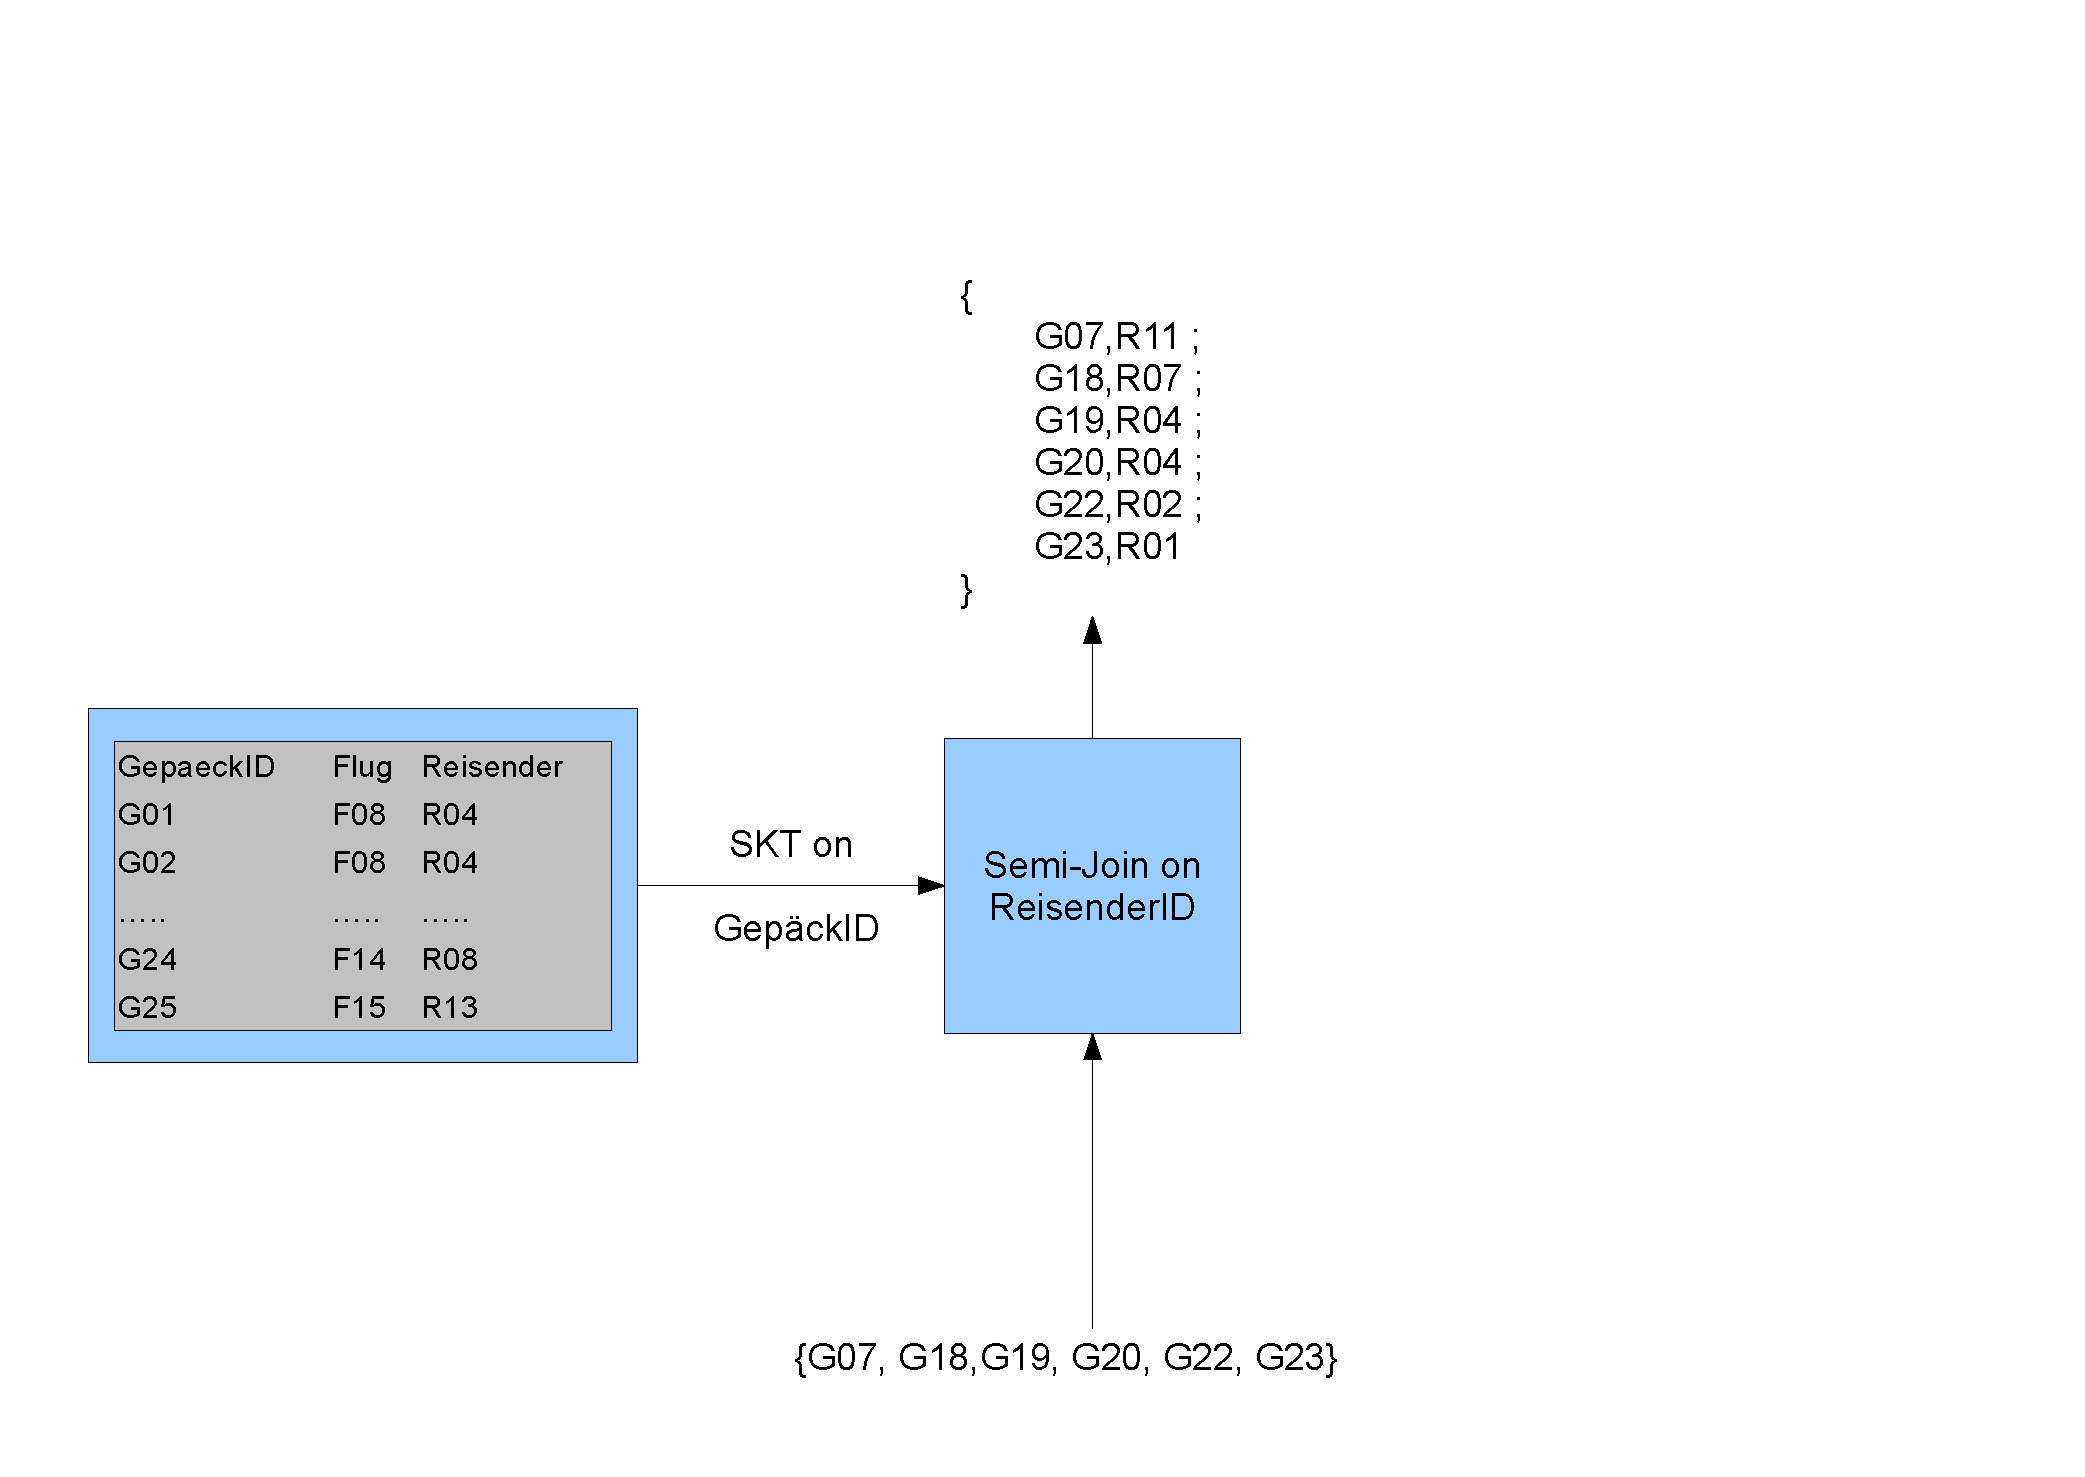
\includegraphics[width=1\textwidth]{img/Post2.pdf}
  \caption{Teilergebnis Post-Filtering 2}
  \label{fig:post2}
\end{figure}

Im n�chsten Schritt kann nun die Selektion auf dem Gep�ck, welches ein Gewicht gr��er als 20 Kilogramm hat geschehen. Wie oben schon erw�hnt wird hierf�r das ``Fuzzy Filtering'' benutzt. In unserem Fall ist es so definiert, das ein Bloomfilter �ber eine bestimmte Menge von Daten generiert wird und dieser Filter dann auf eine andere Menge angewendet wird. Man k�nnte diesen Filter eventuell auf das Ergebnis des Joins beziehen, da diese Ergebnisse aber im sicheren Bereich sind w�rden wir hier nur unn�tig Ressourcen verbrauchen. Eine bessere L�sung ist es den Bloomfilter auf der Selektion der Daten des unsicheren Bereiches zu generieren, da hier mehr Resosurcen zur Verf�gung stehen.

Es wird also ein Bloomfilter auf dem Ergebnis von G.Gewicht>20 gebildet und auf folgende Daten des Joins angewendet:\{$\langle$G07,R11$\rangle$, $\langle$G18,R07$\rangle$, $\langle$G19,R04$\rangle$, $\langle$G20,R04$\rangle$, $\langle$G22,R02$\rangle$, $\langle$G23,R01$\rangle$\}.

Hierbei ist zu beachten das nur die GepaeckIDs des Ergebnisses betrachtet werden, da nur diese im Bloomfilter vorkommen. Auf der Ausgabe des Bloomfilters wird nachfolgend noch eine Projektion auf die ReisendeIDs vorgenommen, da wir die Tupel aus GepaeckID und ReisendeID nicht mehr f�r die n�chsten Schritte ben�tigen. Das Ergebnis sind folgende ReisendeIDs: {R07, R04, R04, R02, R01}

\textbf{TODO: bessere Skalierung f�r das Bild w�hlen}
\begin{figure}[htbp]
  \centering
  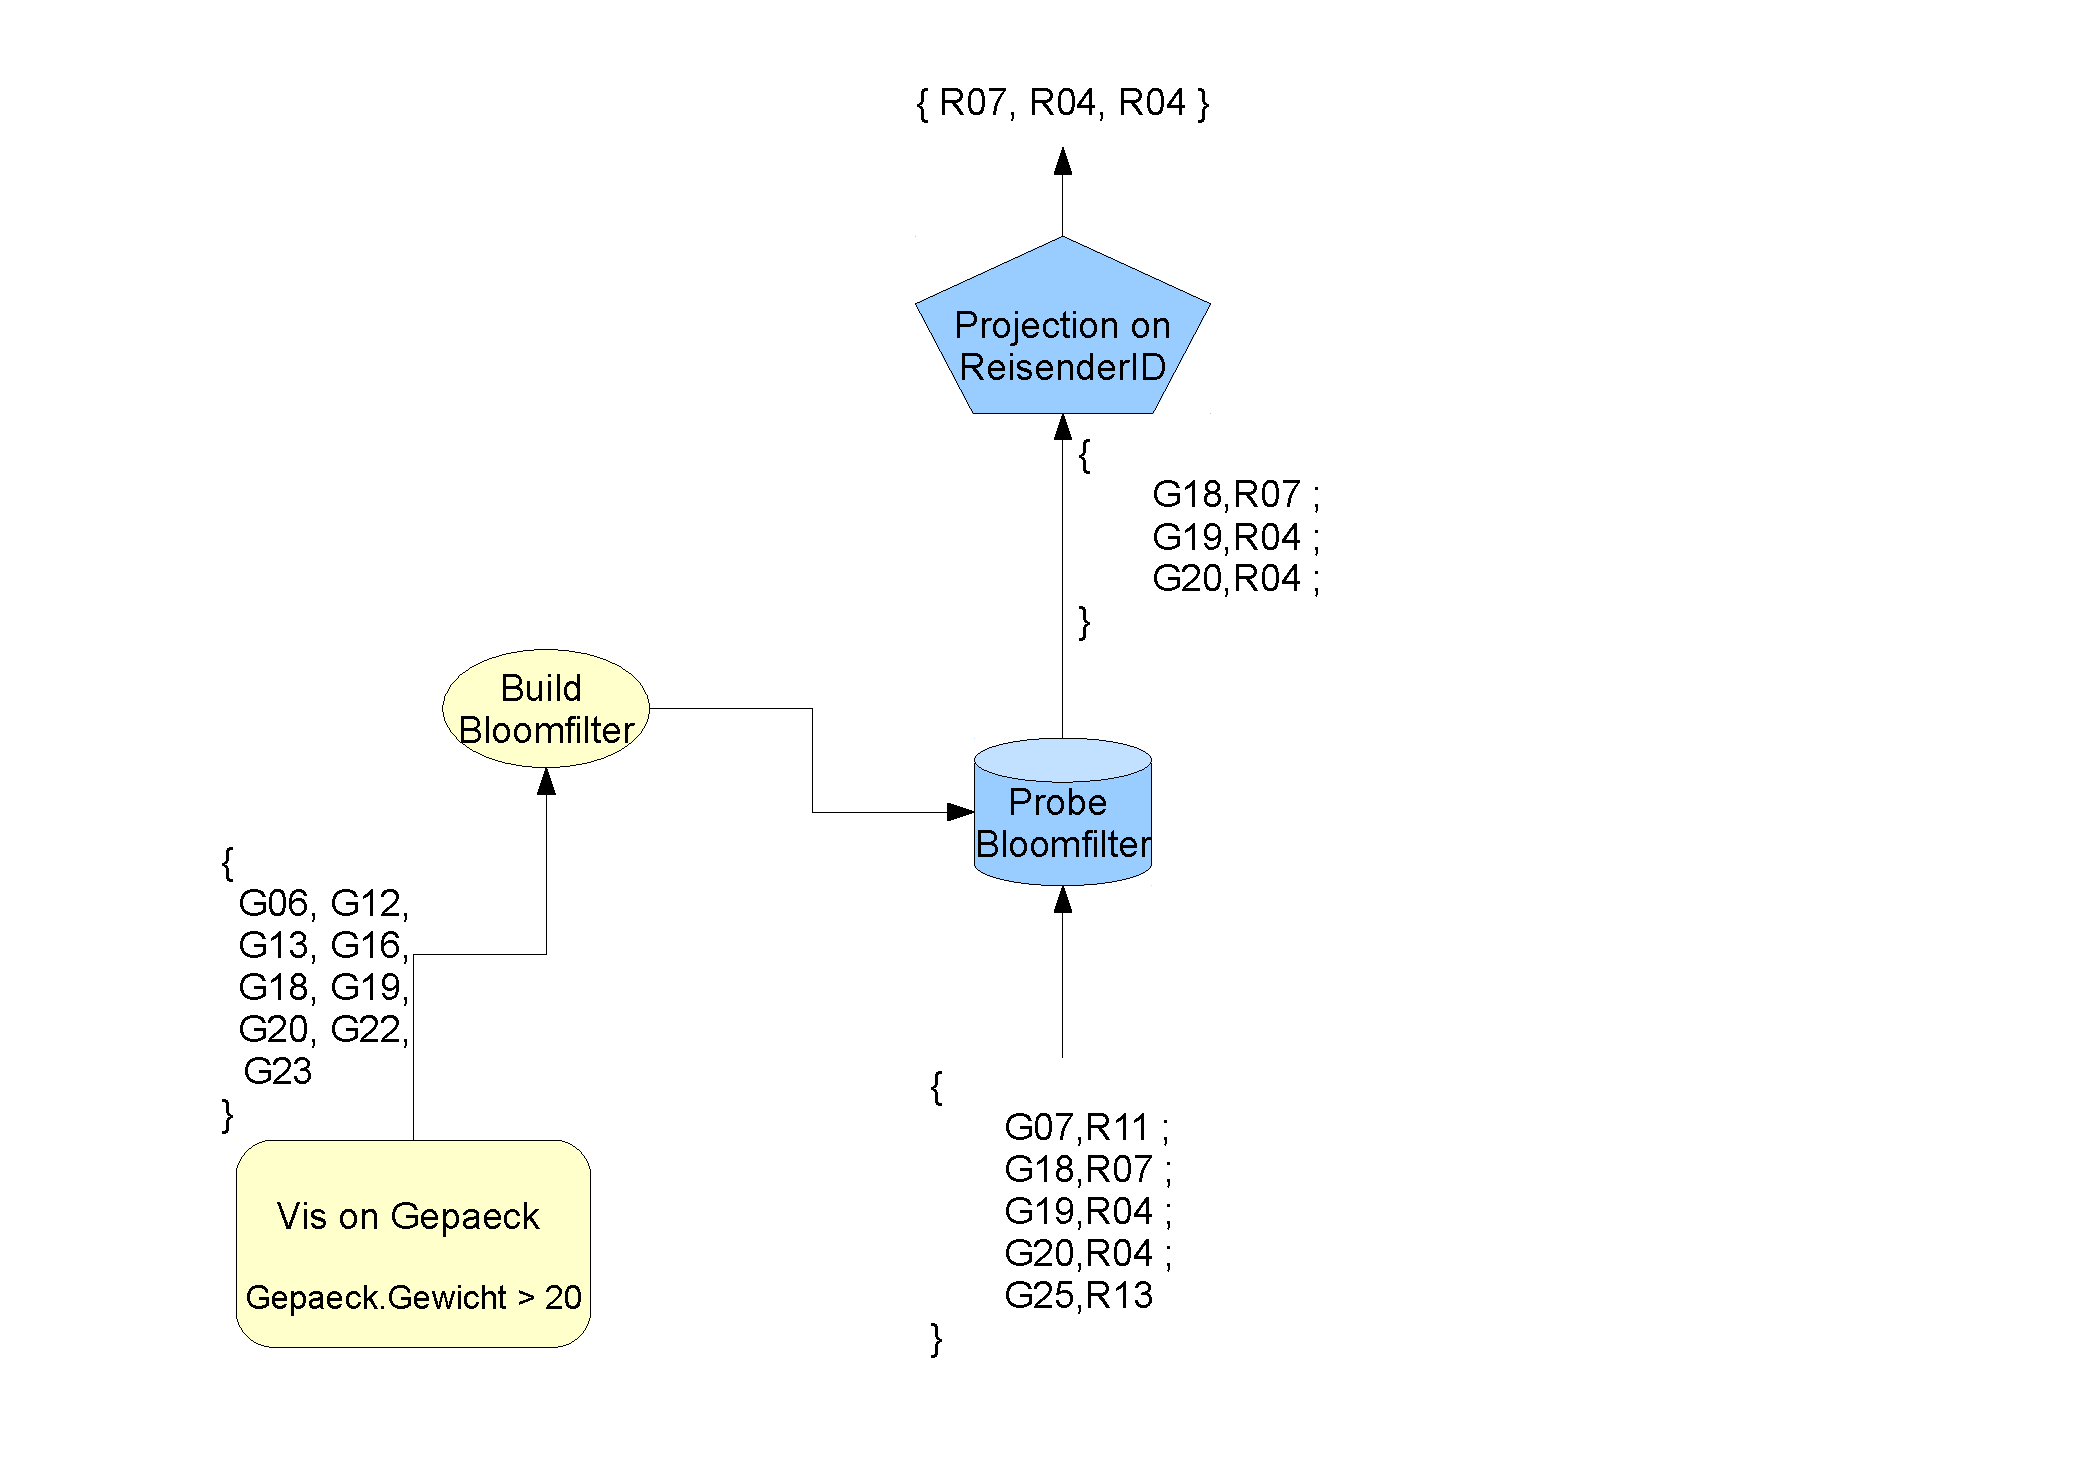
\includegraphics[width=1\textwidth]{img/Post3.pdf}
  \caption{Teilergebnis Post-Filtering 3}
  \label{fig:post3}
\end{figure}

Als n�chster logischer Schritt w�rde die Selektion auf dem Geschlecht folgen, da aber durch die ``Where-Clause'' B.Reisender=R.ReisenderID ebenfalls ReisendeIds entstehen, die verglichen werden m�ssen, wird dieser Schritt vorgezogen, da andernfalls die Selektion ein zweites Mal erfolgen m�sste. Diesen Mehraufwand wollen wir uns ersparen. Um die entsprechende ``Where-Clause'' zu erf�llen, ben�tigen wir BuchungsIDs, die wir dann in entsprechende ReisendeIDs umwandeln k�nnen. Hier verwenden wir das gleiche Schema wie im Prefiltering. Mittels der Selektion auf dem Geburtsdatum des Piloten erhalten wir durch den ``Climbing Index'' eine Liste von Listen mit BuchungsIds. Diese muss durch eine Vereinigung zu einer Liste zusammengef�hrt werden.

Im folgenden wird ein SemiJoin angewendet, der unter Zuhilfenahme eines ``Subtree Key Tables'' uns die entsprechenden ReisendeIDs ausgibt, die wir dann weiterverwenden. Als Ergebnis werden folgende Ids geliefert: {R07, R03, R13, R05, R04, R11}

\textbf{TODO: bessere Skalierung f�r das Bild w�hlen}
\begin{figure}[htbp]
  \centering
  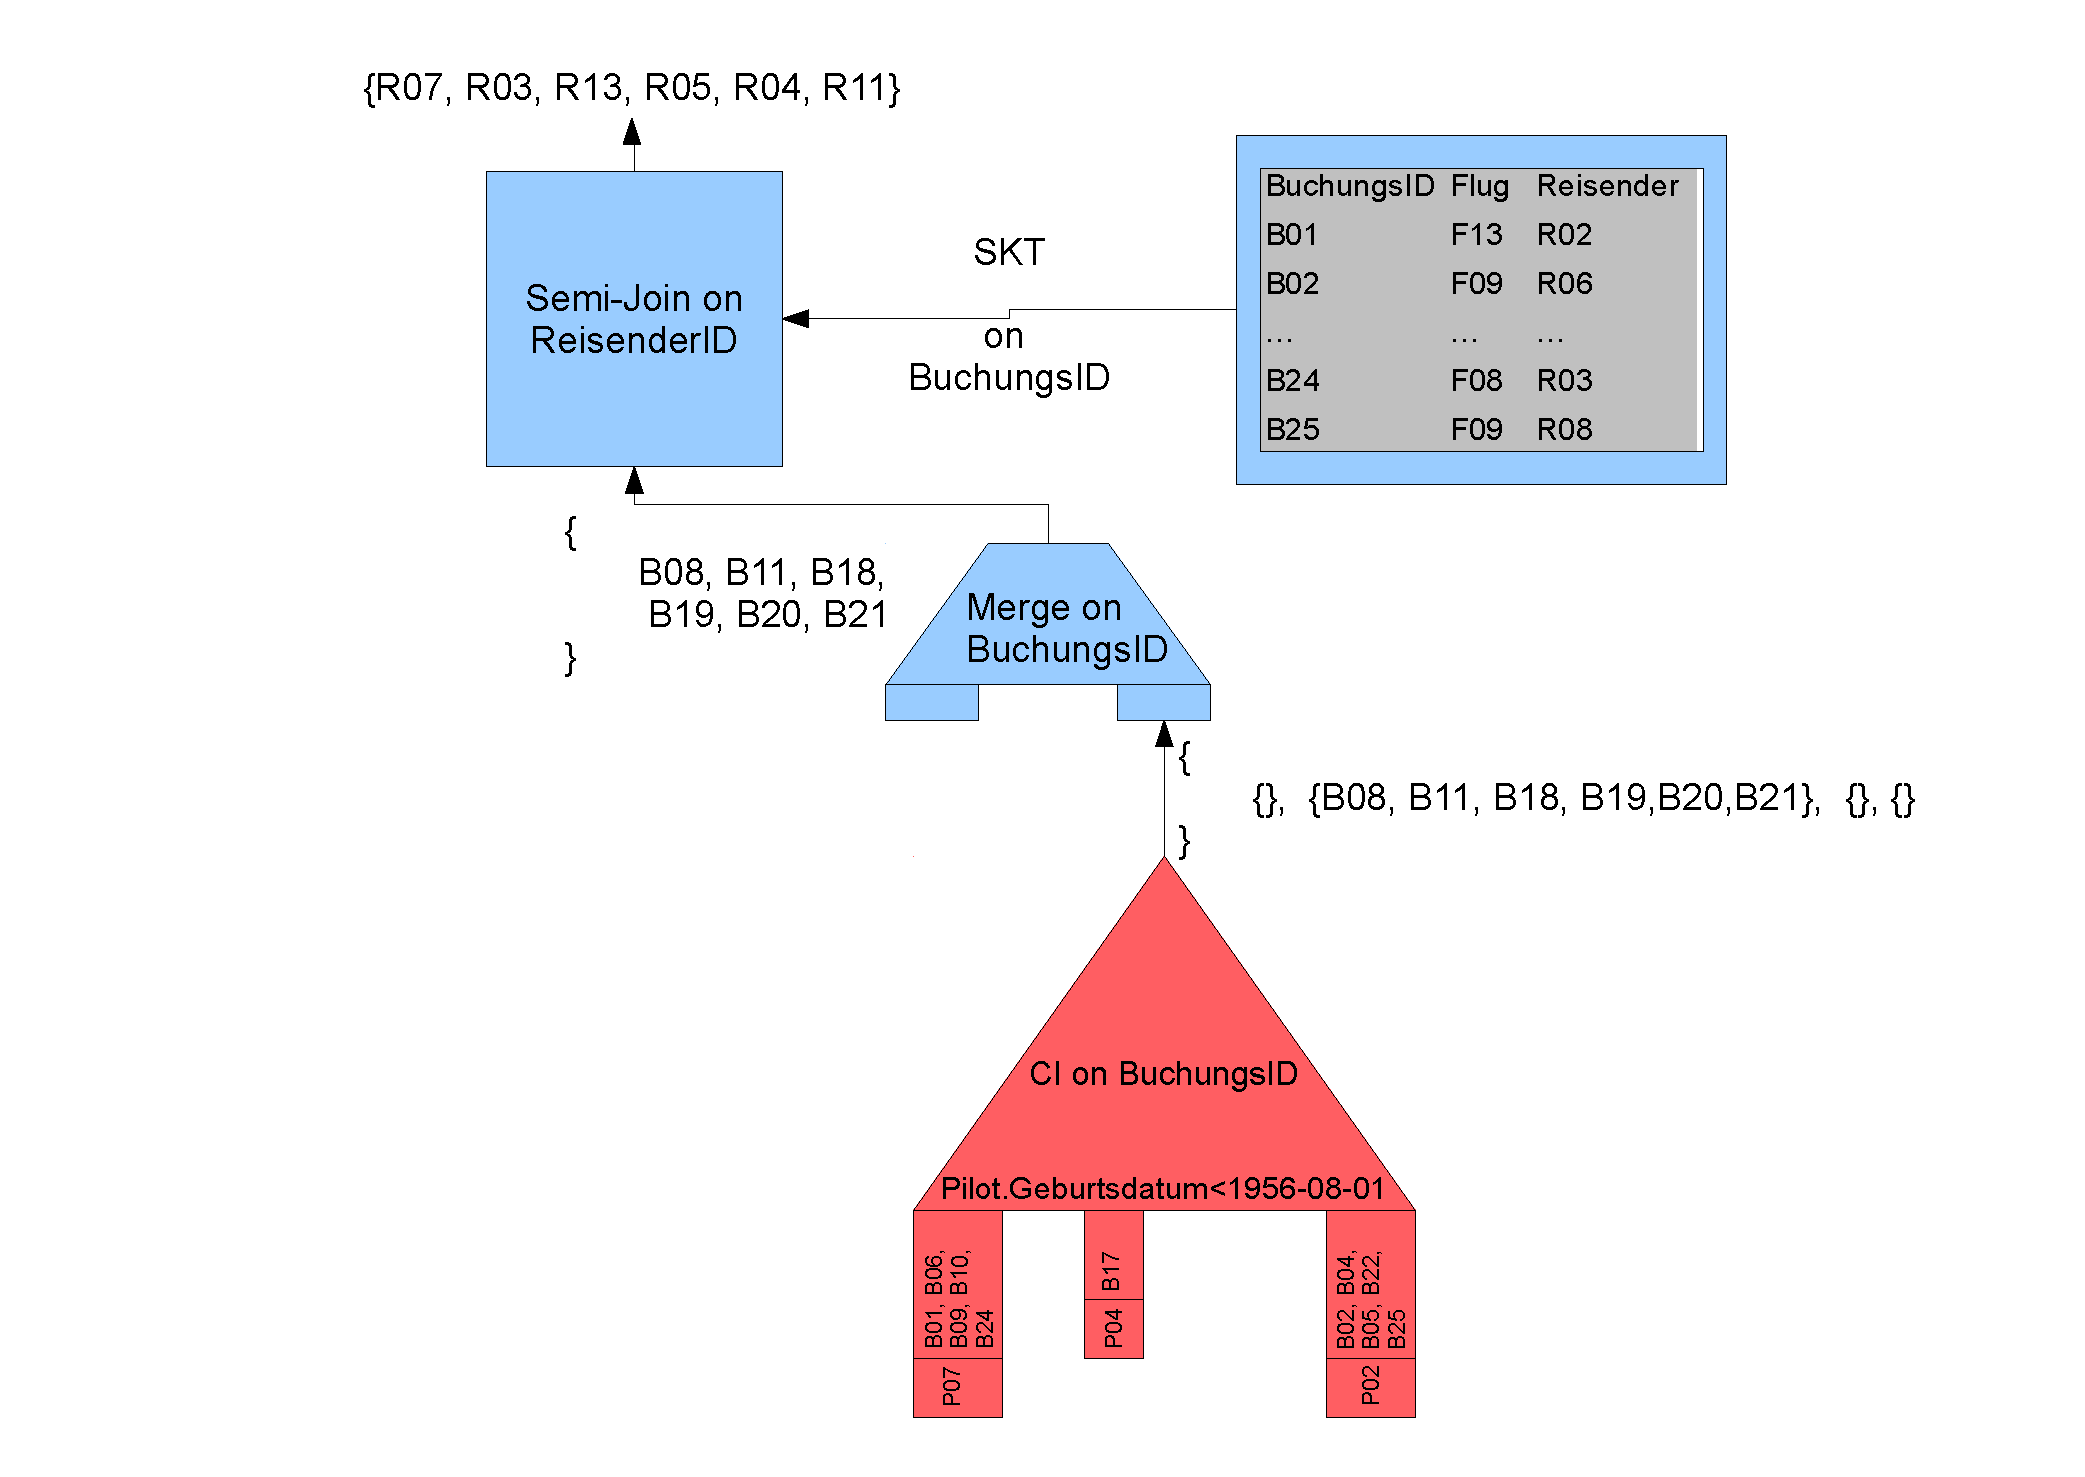
\includegraphics[width=1\textwidth]{img/Post4.pdf}
  \caption{Teilergebnis Post-Filtering 4}
  \label{fig:post4}
\end{figure}

Die beiden Mengen von ReisendeIDs werden nun mittels Durchschnitt miteinander vereint. Aus diesem Ergebnis wird nachfolgend einen Bloomfilter gebaut. Die Ergebnisse die durch die Selektion des Geschlechtes auf die Reisenden (Reisender.Geschlecht='M') im unsicheren Bereich erhaltenen Daten werden durch diesen Filter geschickt. Die nun erhaltenen IDs werden wie im Prefiltering mittels MJoin zusammengef�gt und als Ergebnis erh�lt man: \{$\langle$R04,Doru,Davidovici,Rom�nisch$\rangle$\}.

\textbf{TODO: bessere Skalierung f�r das Bild w�hlen}
\begin{figure}[htbp]
  \centering
  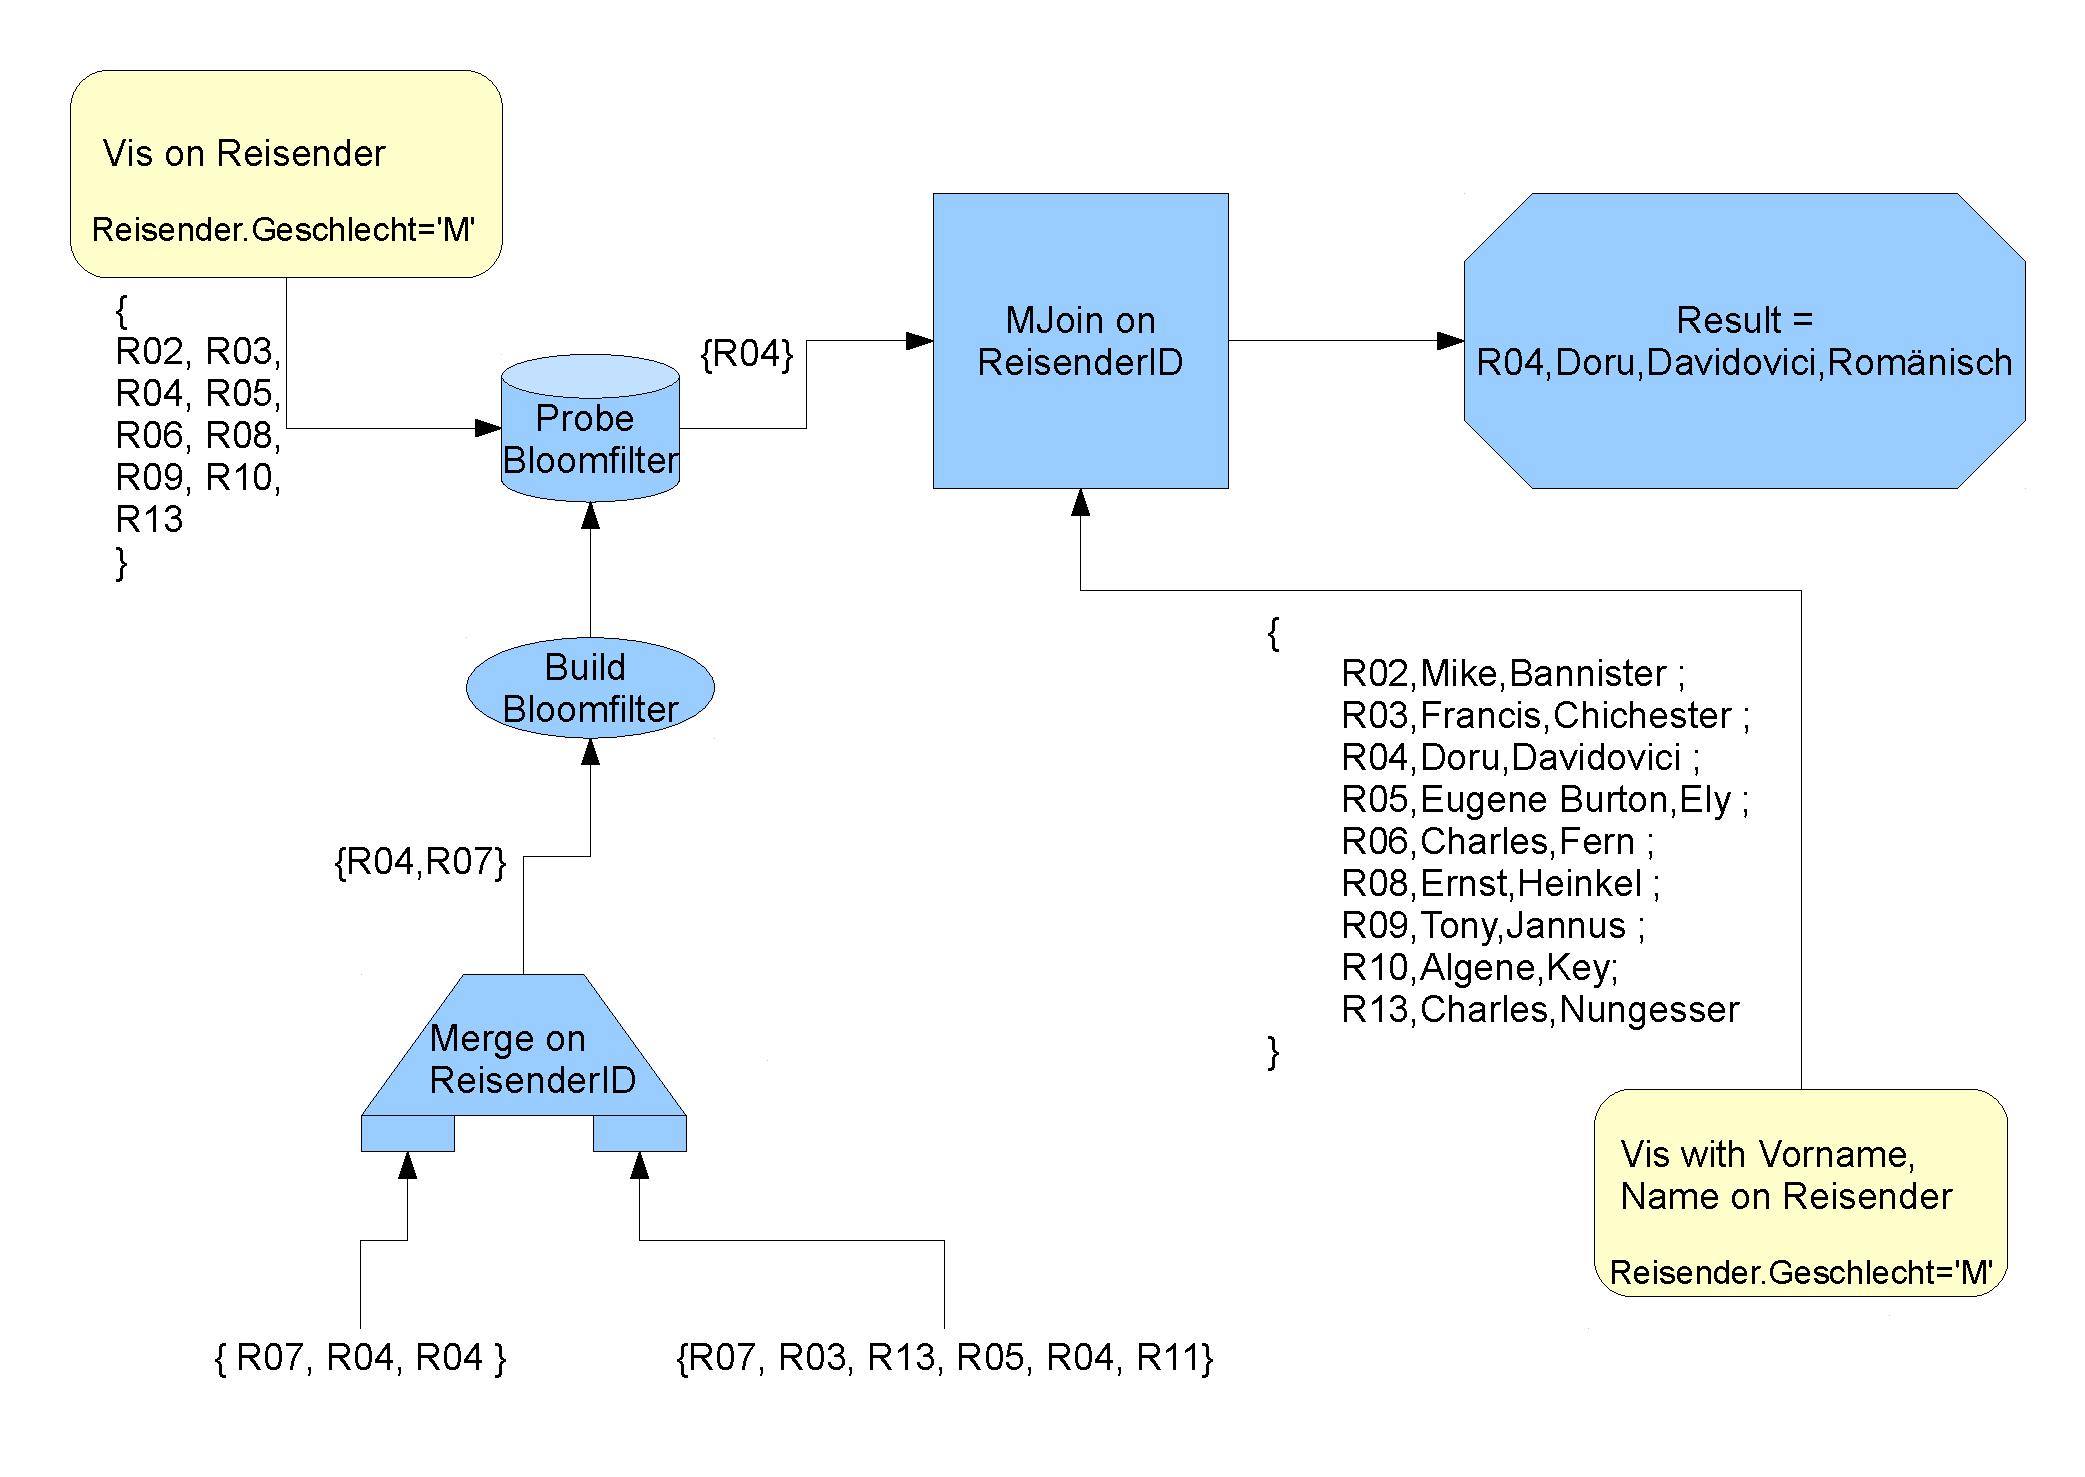
\includegraphics[width=1\textwidth]{img/Post5.pdf}
  \caption{Teilergebnis Post-Filtering 5}
  \label{fig:post5}
\end{figure}

F�gt man nun wie schon oben alle Teile zusammen erh�lt man den kompletten Ablaufplan f�r unsere Anfrage.

\textbf{TODO: bessere Skalierung f�r das Bild w�hlen}
\begin{figure}[htbp]
  \centering
  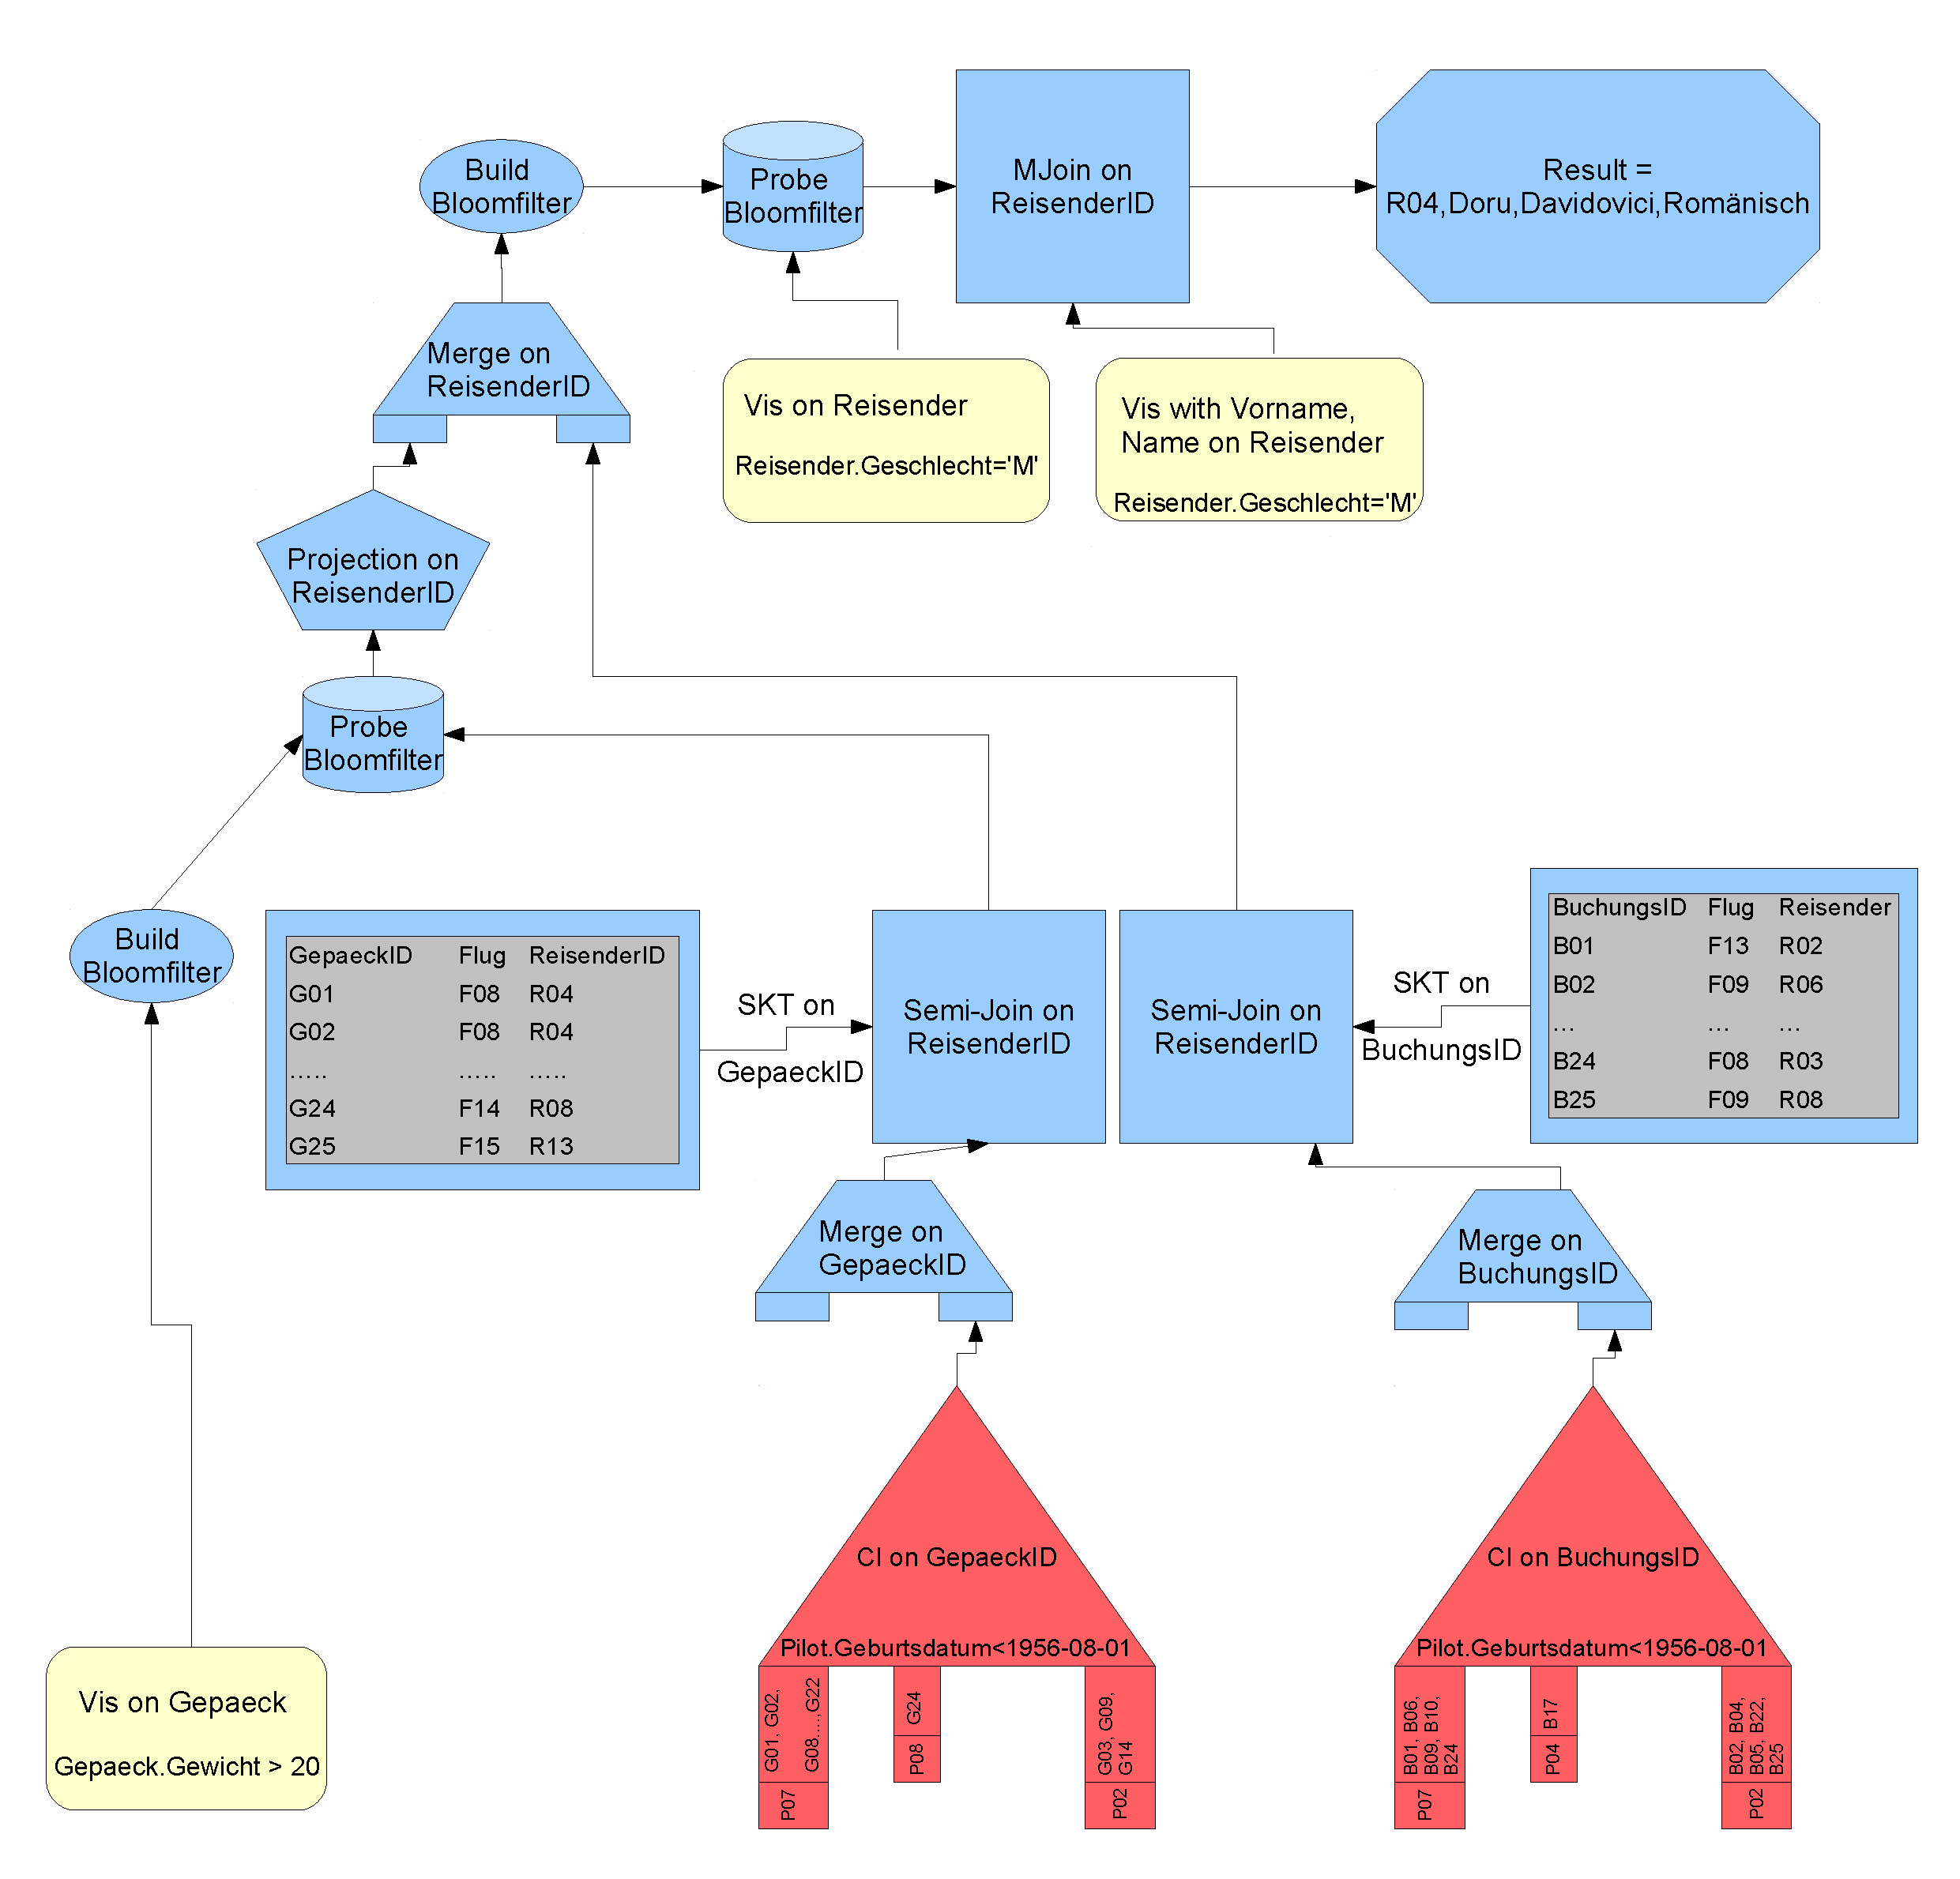
\includegraphics[width=1\textwidth]{img/Post-Filtering.pdf}
  \caption{Post-Filtering QEP}
  \label{fig:post}
\end{figure}

\chapter{Datenbank}
In den entsprechenden Papern zu diesem Thema wurden meist Beispiele aus dem medizinischen Bereich mit �rzten, Patienten, Untersuchungen und mehr gew�hlt. Wir haben uns f�r ein anderes Feld entschieden: den Flugverkehr. Hier existieren viele verschiedene Daten, die je nach Angreifermodell und Nutzer zu sch�tzen sind. Eine Fluggesellschaft ist zum Beispiel daran interessiert, welche Reisende ihr Kontingent an Gep�ckst�cken beziehungsweise Gewicht �berschreiten, um ihnen beim n�chsten Flug ein teureres Ticket verkaufen zu k�nnen. Andererseits soll aber nicht f�r jeden erkennbar sein wer, wann, wohin geflogen ist.

Die von uns erdachte Datenbank besteht aus 6 Tabellen: \textit{Buchungen}, \textit{Gepaeck}, \textit{Fluege}, \textit{Reisende}, \textit{Flugzeuge} und \textit{Piloten}. Die jeweils enthaltenen Attribute sind in den Tabellen \ref{tab:SchemaBuchungen} bis \ref{tab:SchemaPiloten} zu sehen. Grau hinterlegte Attribute, h�ufig Fremdschl�ssel, m�ssen unserer Meinung nach besonders gesch�tzt werden und werden deshalb auf dem ``SmartUSB''-Stick gespeichert.

\begin{table}[H]
\centering
\begin{tabular}{|l|}
\hline
\bfseries Buchungen\\
\hline
BuchungsID\\
Datum\\
Preis\\
Flug\\
\cellcolor[rgb]{0.85,0.85,0.85}Reisender\\
\hline
\end{tabular}
\caption{Schema Buchungen}
\label{tab:SchemaBuchungen}
\end{table}

\begin{table}[H]
\centering
\begin{tabular}{|l|}
\hline
\bfseries Gepaeck\\
\hline
GepaeckID\\
Flug\\
Gewicht\\
Abgabe\\
\cellcolor[rgb]{0.85,0.85,0.85}Reisender\\
\hline
\end{tabular}
\caption{Schema Gepaeck}
\label{tab:SchemaGepaeck}
\end{table}

\begin{table}[H]
\centering
\begin{tabular}{|l|}
\hline
\bfseries Fluege\\
\hline
FlugID\\
Start\\
Ziel\\
Entfernung\\
Abflug\\
Flugzeug\\
\cellcolor[rgb]{0.85,0.85,0.85}Pilot\\
\hline
\end{tabular}
\caption{Schema Fluege}
\label{tab:SchemaFluege}
\end{table}

\begin{table}[H]
\centering
\begin{tabular}{|l|}
\hline
\bfseries Reisende\\
\hline
ReisenderID\\
Vorname\\
Name\\
Geschlecht\\
\cellcolor[rgb]{0.85,0.85,0.85}Geburtsdatum\\
\cellcolor[rgb]{0.85,0.85,0.85}Staatsbuergerschaft\\
\hline
\end{tabular}
\caption{Schema Reisende}
\label{tab:SchemaReisende}
\end{table}

\begin{table}[H]
\centering
\begin{tabular}{|l|}
\hline
\bfseries Flugzeuge\\
\hline
FlugzeugID\\
Typ\\
Reichweite\\
Sitzplaetze\\
\hline
\end{tabular}
\caption{Schema Flugzeuge}
\label{tab:SchemaFlugzeuge}
\end{table}

\begin{table}[H]
\centering
\begin{tabular}{|l|}
\hline
\bfseries Piloten\\
\hline
PilotID\\
Vorname\\
Name\\
Geschlecht\\
\cellcolor[rgb]{0.85,0.85,0.85}Geburtsdatum\\
\cellcolor[rgb]{0.85,0.85,0.85}Gehalt\\
\hline
\end{tabular}
\caption{Schema Piloten}
\label{tab:SchemaPiloten}
\end{table}

Visualisiert man die Fremdschl�sselbeziehungen zwischen den Tabellen mit Pfeilen ergibt sich die Struktur in Abbildung \ref{fig:Datenmodell}. Die hier verwendete Datenbank unterscheidet sich strukturell stark von dem Beispiel, dass die ``GhostDB''-Autoren verwendeten. Am Auff�lligsten ist das Vorhandensein von zwei ``Wurzeln''. In den zugrunde liegenden Arbeiten werden explizit nur Datenbanken in Baumstrukur, das hei�t mit einer Wurzel, vorgesehen. Dies sahen wir als Herausforderung das ``GhostDB''-System daran zu erproben. Erstaunlicherweise entstanden dadurch kaum Probleme. In der Anfragebearbeitung waren aber teilweise zus�tzliche Schritte n�tig.

\begin{figure}[htbp]
\centering
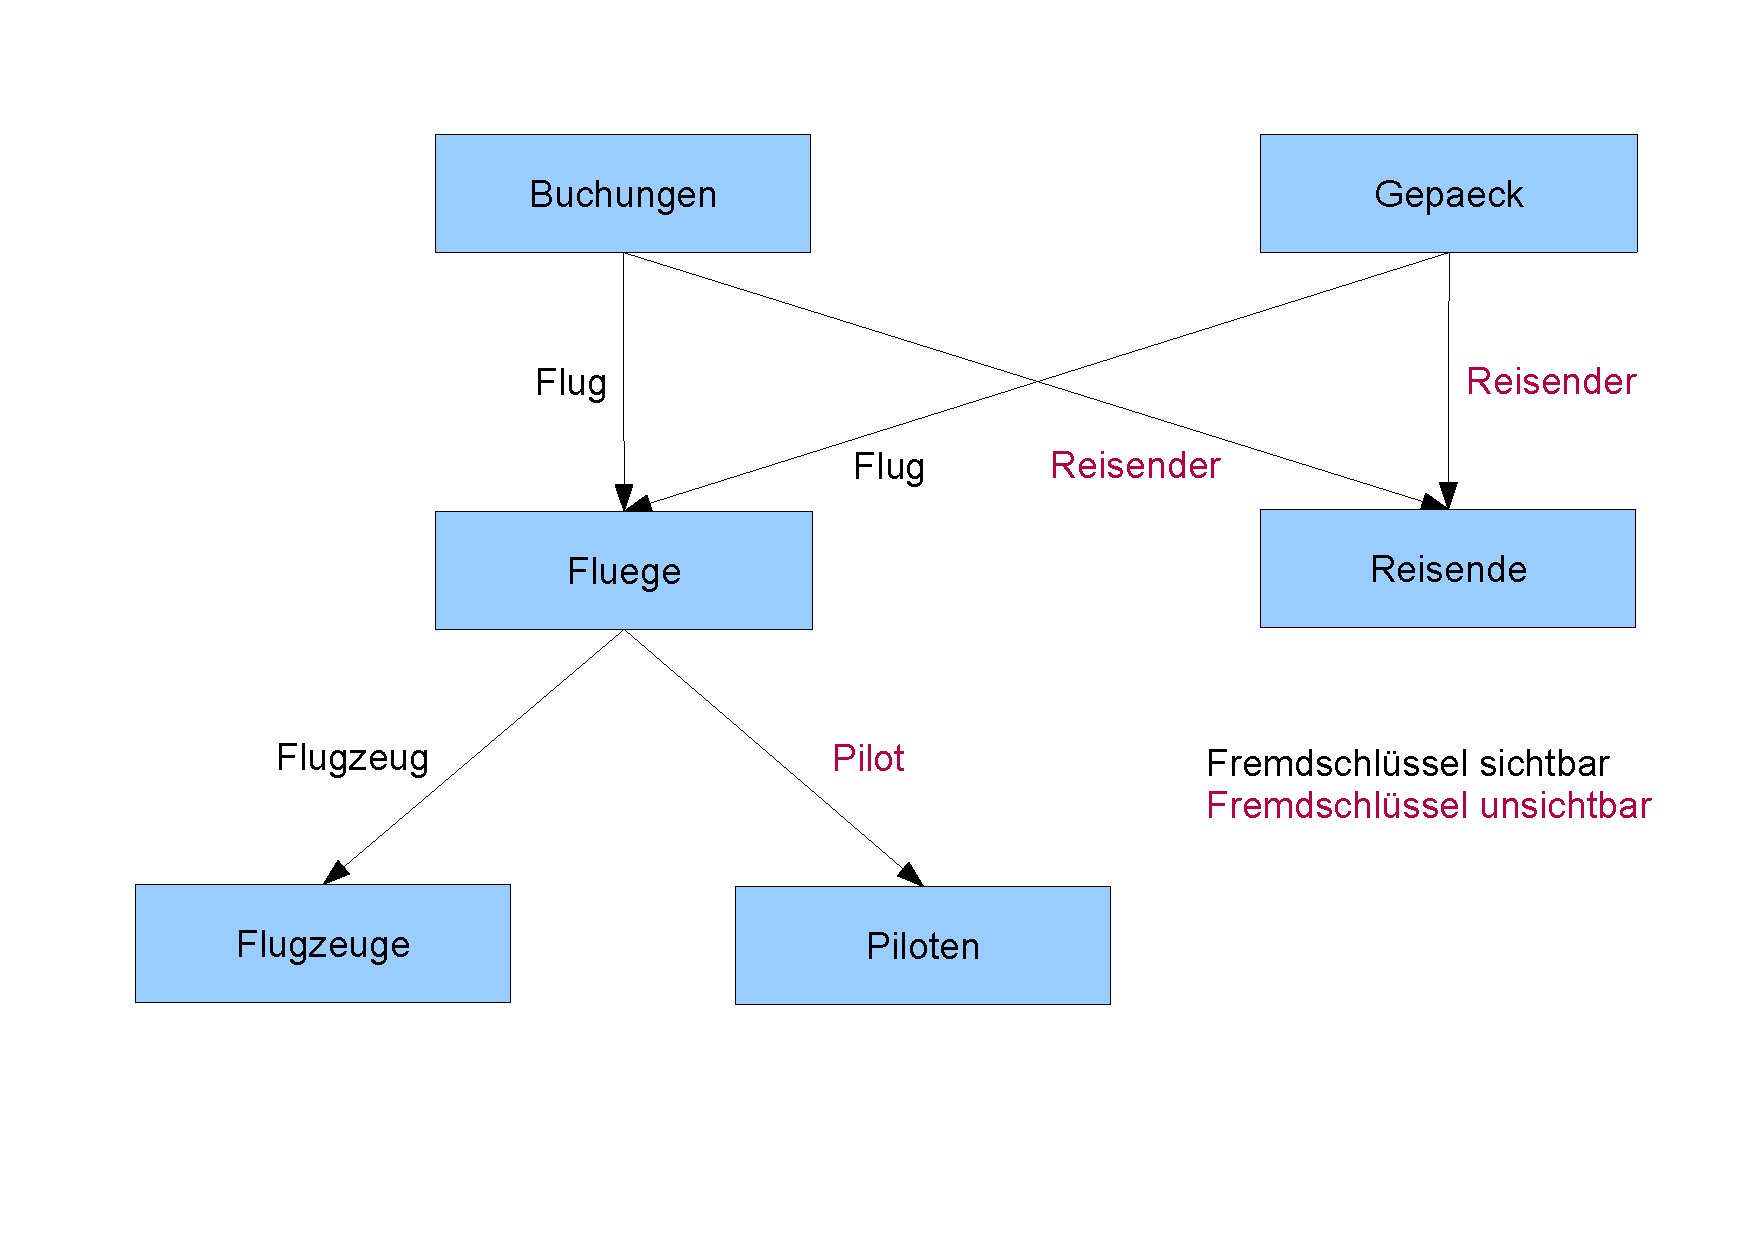
\includegraphics[width=1.00\textwidth]{img/Datenmodell.pdf}
\caption{Datenmodell}
\label{fig:Datenmodell}
\end{figure}

Um die verwendeten Strukturen, ``Subtree Key Table'' und ``Climbing Index'', ad�quat vorzustellen, haben wir die ausgedachten Tabellen mit Daten bef�llt. Dies ist in den Tabllen \ref{tab:Buchungen} bis \ref{tab:Piloten} dargestellt. Einige Tabellen enthalten Attribute, die nicht frei erfunden sind, insbesondere Personen und Orte. Die dabei verwendeten Quellen sind im Anhang aufgelistet.

\begin{table}[htbp]
\centering
\begin{tabular}{|c|c|c|c|c|}
\hline
\bfseries BuchungsID&\bfseries Datum&\bfseries Preis&\bfseries Flug&\bfseries Reisender\\
\hline
B01&2010-12-08&342&F13&R02\\
\hline
B02&2011-01-04&226&F09&R06\\
\hline
B03&2011-01-23&241&F06&R01\\
\hline
B04&2011-03-15&469&F09&R15\\
\hline
B05&2011-04-04&339&F02&R13\\
\hline
B06&2011-05-13&490&F13&R03\\
\hline
B07&2011-05-18&109&F10&R11\\
\hline
B08&2011-05-18&137&F15&R07\\
\hline
B09&2011-05-20&66&F13&R09\\
\hline
B10&2011-06-04&220&F08&R04\\
\hline
B11&2011-06-15&222&F15&R03\\
\hline
B12&2011-06-22&147&F06&R02\\
\hline
B13&2011-06-22&147&F06&R14\\
\hline
B14&2011-06-22&65&F06&R09\\
\hline
B15&2011-07-01&319&F01&R10\\
\hline
B16&2011-07-09&380&F14&R08\\
\hline
B17&2011-07-14&394&F03&R12\\
\hline
B18&2011-07-26&161&F15&R13\\
\hline
B19&2011-08-05&325&F15&R05\\
\hline
B20&2011-08-09&257&F05&R04\\
\hline
B21&2011-08-09&257&F05&R11\\
\hline
B22&2011-08-10&432&F09&R01\\
\hline
B23&2011-08-13&157&F14&R10\\
\hline
B24&2011-08-22&90&F08&R03\\
\hline
B25&2011-08-23&416&F09&R08\\
\hline
\end{tabular}
\caption{Buchungen}
\label{tab:Buchungen}
\end{table}

\begin{table}[htbp]
\centering
\begin{tabular}{|c|c|c|c|c|}
\hline
\bfseries GepaeckID&\bfseries Flug&\bfseries Gewicht&\bfseries Abgabe&\bfseries Reisender\\
\hline
G01&F08&14&2011-08-20 17:05&R04\\
\hline
G02&F08&10&2011-08-20 17:05&R04\\
\hline
G03&F09&15&2011-08-23 09:30&R01\\
\hline
G04&F10&16&2011-08-16 07:31&R11\\
\hline
G05&F06&14&2011-08-09 12:58&R02\\
\hline
G06&F06&21&2011-08-09 12:58&R14\\
\hline
G07&F05&14&2011-08-09 13:00&R11\\
\hline
G08&F08&20&2011-08-22 21:47&R04\\
\hline
G09&F09&20&2011-08-23 08:45&R15\\
\hline
G10&F13&15&2011-08-23 20:20&R02\\
\hline
G11&F10&11&2011-08-23 14:35&R11\\
\hline
G12&F08&21&2011-08-21 07:59&R03\\
\hline
G13&F10&23&2011-08-23 12:07&R11\\
\hline
G14&F09&14&2011-08-22 21:47&R08\\
\hline
G15&F01&12&2011-08-02 00:45&R10\\
\hline
G16&F01&21&2011-08-02 00:45&R10\\
\hline
G17&F13&17&2011-08-26 16:42&R09\\
\hline
G18&F15&21&2011-08-30 12:40&R07\\
\hline
G19&F05&22&2011-08-08 23:57&R04\\
\hline
G20&F05&25&2011-08-08 23:57&R04\\
\hline
G21&F08&10&2011-08-21 08:00&R03\\
\hline
G22&F13&22&2011-08-25 22:42&R02\\
\hline
G23&F06&25&2011-08-14 04:19&R01\\
\hline
G24&F14&18&2011-08-27 21:13&R08\\
\hline
G25&F15&16&2011-08-29 17:55&R13\\
\hline
\end{tabular}
\caption{Gepaeck}
\label{tab:Gepaeck}
\end{table}

\begin{sidewaystable}[htbp]
\centering
\begin{tabular}{|c|c|c|c|c|c|c|}
\hline
\bfseries FlugID&\bfseries Start&\bfseries Ziel&\bfseries Entfernung&\bfseries Abflug&\bfseries Flugzeug&\bfseries Pilot\\
\hline
F01&Berlin (SXF)&Antwerpen (ANR)&638&2011-08-02 04:25&A05&P03\\
\hline
F02&Berlin (SXF)&Barcelona (BCN)&1506&2011-08-05 16:10&A01&P02\\
\hline
F03&Berlin (SXF)&Chicago (ORD)&7118&2011-08-08 19:45&A02&P04\\
\hline
F04&Berlin (SXF)&Dortmund (DTM)&417&2011-08-09 04:05&A05&P02\\
\hline
F05&Berlin (SXF)&Erfurt (ERF)&236&2011-08-09 15:25&A04&P10\\
\hline
F06&Berlin (SXF)&Florenz (FLR)&968&2011-08-14 07:15&A01&P03\\
\hline
F07&Berlin (SXF)&Genf (GVA)&869&2011-08-19 15:45&A04&P08\\
\hline
F08&Berlin (SXF)&Hamburg (HAM)&275&2011-08-23 06:30&A05&P07\\
\hline
F09&Berlin (SXF)&Istanbul (IST)&1717&2011-08-23 12:25&A03&P02\\
\hline
F10&Berlin (SXF)&Jakarta (CGK)&10745&2011-08-23 15:20&A02&P06\\
\hline
F11&Berlin (SXF)&Kiew (KBP)&1227&2011-08-23 18:30&A04&P04\\
\hline
F12&Berlin (SXF)&London (LHR)&965&2011-08-26 13:20&A01&P01\\
\hline
F13&Berlin (SXF)&Madrid (MAD)&1853&2011-08-26 18:15&A03&P07\\
\hline
F14&Berlin (SXF)&New York (JFK)&6401&2011-08-29 00:30&A02&P08\\
\hline
F15&Berlin (SXF)&Oslo (OSL)&882&2011-08-30 15:20&A01&P10\\
\hline
\end{tabular}
\caption{Fluege}
\label{tab:Fluege}
\end{sidewaystable}

\begin{sidewaystable}[htbp]
\centering
\begin{tabular}{|c|c|c|c|c|c|}
\hline
\bfseries ReisenderID&\bfseries Vorname&\bfseries Name&\bfseries Geschlecht&\bfseries Geburtsdatum&\bfseries Staatsbuergerschaft\\
\hline
R01&Jacqueline&Auriol&F&1955-11-05&Franz�sisch\\
\hline
R02&Mike&Bannister&M&1969-10-24&Britisch\\
\hline
R03&Francis&Chichester&M&1939-09-17&Britisch\\
\hline
R04&Doru&Davidovici&M&1987-04-20&Rom�nisch\\
\hline
R05&Eugene Burton&Ely&M&1971-10-21&US-Amerikanisch\\
\hline
R06&Charles&Fern&M&1942-02-01&US-Amerikanisch\\
\hline
R07&Sabiha&G�k�en&F&1978-03-22&T�rkisch\\
\hline
R08&Ernst&Heinkel&M&1936-01-24&Deutsch\\
\hline
R09&Tony&Jannus&M&2008-07-22&US-Amerikanisch\\
\hline
R10&Algene&Key&M&1945-06-04&US-Amerikanisch\\
\hline
R11&Ruth Bancroft&Law&F&1984-11-19&US-Amerikanisch\\
\hline
R12&Marie&Marvingt&F&1966-02-20&Franz�sisch\\
\hline
R13&Charles&Nungesser&M&1964-03-15&Franz�sisch\\
\hline
R14&Ivy May&Pearce&F&1969-06-08&Australisch\\
\hline
R15&Harriet&Quimby&F&1980-05-01&US-Amerikanisch\\
\hline
\end{tabular}
\caption{Reisende}
\label{tab:Reisende}
\end{sidewaystable}

\begin{table}[htbp]
\centering
\begin{tabular}{|c|c|c|c|}
\hline
\bfseries FlugzeugID&\bfseries Typ&\bfseries Reichweite&\bfseries Sitzplaetze\\
\hline
A01&Airbus A300B4&6670&266\\
\hline
A02&Airbus A340-200&15000&240\\
\hline
A03&Boeing 747-200B&12700&366\\
\hline
A04&Bombardier CRJ100 LR&3710&50\\
\hline
A05&Bombardier CRJ1000&2491&100\\
\hline
\end{tabular}
\caption{Flugzeuge}
\label{tab:Flugzeuge}
\end{table}

\begin{table}[htbp]
\centering
\begin{tabular}{|c|c|c|c|c|c|}
\hline
\bfseries PilotID&\bfseries Vorname&\bfseries Name&\bfseries Geschlecht&\bfseries Geburtsdatum&\bfseries Gehalt\\
\hline
P01&John&Alcock&M&1949-11-05&3800\\
\hline
P02&Richard&Bach&M&1978-06-23&2300\\
\hline
P03&George&Cayley&M&1960-12-27&12000\\
\hline
P04&Jimmy&Doolittle&M&1964-12-14&5100\\
\hline
P05&Amelia&Earhart&F&1956-07-24&8400\\
\hline
P06&Henri&Farman&M&1974-05-26&6700\\
\hline
P07&Roland&Garros&M&1959-10-06&10000\\
\hline
P08&Hilda&Hewlett&F&1967-02-17&6700\\
\hline
P09&Amy&Johnson&F&1948-07-01&8300\\
\hline
P10&Fred&Key&M&1945-06-04&6000\\
\hline
\end{tabular}
\caption{Piloten}
\label{tab:Piloten}
\end{table}

\chapter{Subtree Key Table}
Um Joins zu beschleunigen werden in ``GhostDB'' Join Indizes, so genannte ``Subtree Key Tables'', benutzt. F�r alle Tabellen mit ``Nachfahren'', das hei�t Tabellen, die Fremdschl�ssel enthalten, kann ein ``Subtree Key Table'' erstellt werden. Dieser enth�lt den Prim�rschl�ssel der Tabelle selbst, sowie die dazugeh�rigen Fremdschl�ssel und die Fremdschl�ssel der Fremdschl�ssel etc. Der ``Subtree Key Table'', der zur Tabelle Buchungen geh�rt, hat als Prim�rschl�ssel \textit{BuchungsID}. Darauf wird dieser ``Subtree Key Table'' sortiert. Zu jeder \textit{BuchungsID} wird die passende \textit{FlugID} und \textit{ReisenderID} in der entsprechenden Spalte eingetragen. Zu der soeben bestimmten \textit{FlugID} werden au�erdem die dazugeh�rige \textit{FlugzeugID} und \textit{PilotID} eingetragen. 

Die Verweundung dieser Struktur erm�glicht Joins von der zum ``Subtree Key Table'' geh�rigen Tabelle mit beliebigen Nachfahren in einem Schritt durchzuf�hren, beispielsweise \textit{Buchungen} mit \textit{Piloten}. Die ``Subtree Key Tables'' der Tabellen \textit{Buchungen}, \textit{Gepaeck} und \textit{Fluege} sind in den Tabellen \ref{tab:SKTBuchungen} bis \ref{tab:SKTFluege} dargestellt. Zu den Tabellen \textit{Flugzeuge}, \textit{Piloten} und \textit{Reisende} k�nnen keine ``Subtree Key Tables'' erstellt werden, da diese keine Nachfolger haben.

\begin{table}[htbp]
\centering
\begin{tabular}{|c|c|c|c|c|}
\hline
\bfseries BuchungsID&\bfseries FlugID&\bfseries ReisenderID&\bfseries FlugzeugID&\bfseries PilotID\\
\hline
B01&F13&R02&A03&P07\\
\hline
B02&F09&R06&A03&P02\\
\hline
B03&F06&R01&A01&P03\\
\hline
B04&F09&R15&A03&P02\\
\hline
B05&F02&R13&A01&P02\\
\hline
B06&F13&R03&A03&P07\\
\hline
B07&F10&R11&A02&P06\\
\hline
B08&F15&R07&A01&P10\\
\hline
B09&F13&R09&A03&P07\\
\hline
B10&F08&R04&A05&P07\\
\hline
B11&F15&R03&A01&P10\\
\hline
B12&F06&R02&A01&P03\\
\hline
B13&F06&R14&A01&P03\\
\hline
B14&F06&R09&A01&P03\\
\hline
B15&F01&R10&A05&P03\\
\hline
B16&F14&R08&A02&P08\\
\hline
B17&F03&R12&A02&P04\\
\hline
B18&F15&R13&A01&P10\\
\hline
B19&F15&R05&A01&P10\\
\hline
B20&F05&R04&A04&P10\\
\hline
B21&F05&R11&A04&P10\\
\hline
B22&F09&R01&A03&P02\\
\hline
B23&F14&R10&A02&P08\\
\hline
B24&F08&R03&A05&P07\\
\hline
B25&F09&R08&A03&P02\\
\hline
\end{tabular}
\caption{Subtree Key Table Buchungen}
\label{tab:SKTBuchungen}
\end{table}

\begin{table}[htbp]
\centering
\begin{tabular}{|c|c|c|c|c|}
\hline
\bfseries GepaeckID&\bfseries FlugID&\bfseries ReisenderID&\bfseries FlugzeugID&\bfseries PilotID\\
\hline
G01&F08&R04&A05&P07\\
\hline
G02&F08&R04&A05&P07\\
\hline
G03&F09&R01&A03&P02\\
\hline
G04&F10&R11&A02&P06\\
\hline
G05&F06&R02&A01&P03\\
\hline
G06&F06&R14&A01&P03\\
\hline
G07&F05&R11&A04&P10\\
\hline
G08&F08&R04&A05&P07\\
\hline
G09&F09&R15&A03&P02\\
\hline
G10&F13&R02&A03&P07\\
\hline
G11&F10&R11&A02&P06\\
\hline
G12&F08&R03&A05&P07\\
\hline
G13&F10&R11&A02&P06\\
\hline
G14&F09&R08&A03&P02\\
\hline
G15&F01&R10&A05&P03\\
\hline
G16&F01&R10&A05&P03\\
\hline
G17&F13&R09&A03&P07\\
\hline
G18&F15&R07&A01&P10\\
\hline
G19&F05&R04&A04&P10\\
\hline
G20&F05&R04&A04&P10\\
\hline
G21&F08&R03&A05&P07\\
\hline
G22&F13&R02&A03&P07\\
\hline
G23&F06&R01&A01&P03\\
\hline
G24&F14&R08&A02&P08\\
\hline
G25&F15&R13&A01&P10\\
\hline
\end{tabular}
\caption{Subtree Key Table Gepaeck}
\label{tab:SKTGepaeck}
\end{table}

\begin{table}[htbp]
\centering
\begin{tabular}{|c|c|c|}
\hline
\bfseries FlugID&\bfseries FlugzeugID&\bfseries PilotID\\
\hline
F01&A05&P03\\
\hline
F02&A01&P02\\
\hline
F03&A02&P04\\
\hline
F04&A05&P02\\
\hline
F05&A04&P10\\
\hline
F06&A01&P03\\
\hline
F07&A04&P08\\
\hline
F08&A05&P07\\
\hline
F09&A03&P02\\
\hline
F10&A02&P06\\
\hline
F11&A04&P04\\
\hline
F12&A01&P01\\
\hline
F13&A03&P07\\
\hline
F14&A02&P08\\
\hline
F15&A01&P10\\
\hline
\end{tabular}
\caption{Subtree Key Table Fluege}
\label{tab:SKTFluege}
\end{table}

\chapter{Climbing Index}
In ``GhostDB'' wird eine zweite Datenstruktur zur Beschleunigung von Joins eingesetzt: der ``Climbing Index''. Diese haben die weitere Eigenschaft, dass Selektionen beschleunigt werden k�nnen. Zu jedem Attribut jeder Tabelle kann ein ``Climbing Index'' angelegt werden. Dieser enth�lt den Wert der Attributes und eine Liste von IDs zur jeder Tabelle, die ein Vorfahr ist. Betrachten wir beispielsweise das Attribut \textit{Geburtsdatum} der Tabelle \textit{Piloten}. Es existieren so viele Tupel, wie es verschiedene Werte, das hei�t Geburtsdaten, gibt. Zu jedem Geburtsdatum werden 4 Listen zugeordnet. Eine Liste von \textit{PilotIDs}: alle Piloten, die an diesem Tag geboren wurden. Eine Liste von \textit{FlugIDs}: alle Fluege, die von einem Piloten mit diesem Geburtsdatum gesteuert werden. Eine Liste von \textit{BuchungsIDs}: alle Buchungen, die einem Flug zugeordnet sind, der von einem Piloten mit diesem Geburtsdatum gesteuert wird. Eine Liste von \textit{GepaeckIDs}: Eine Liste von Gep�ckst�cken, die einem Flug zugeordnet sind, der von einem Piloten mit diesem Geburtsdatum gesteuert wird.

Die Anwendung eines ``Climbing Index'' erlaubt Selektionen auf dem dazugeh�rigen Attribut und einen anschlie�enden Join mit einer beliebigen Tabelle, die Vorfahr ist, in einem Schritt vorzunehmen. Beispielsweise eine Selektion auf \textit{Pilot.Geburtsdatum} und anschlie�ender Join mit \textit{Buchungen}. Zu den Tabellen \textit{Piloten}, \textit{Flugzeuge}, \textit{Reisende}, \textit{Fluege}, \textit{Gepaeck} und \textit{Buchungen} wurde beispielhaft f�r je ein Attribut ein ``Climbing Index'' erstellt. Diese sind in den Tabllen \ref{tab:ClimbingIndexPilotenGeburtsdatum} bis \ref{tab:ClimbingIndexBuchungenDatum} dargestellt. Prinzipiell k�nnte aber f�r jedes Attribut dieser Tabellen ein Climbing Index erstellt werden. Es k�nnten also 33 ``Climbing Indices'' f�r unsere Datenbank erstellt werden.

\newcolumntype{C}{>{\centering\arraybackslash}X}
\begin{sidewaystable}[htbp]
\centering
\begin{tabularx}{\textwidth}{|C|C|C|C|C|}
\hline
\bfseries Geburtsdatum&\bfseries PilotIDs&\bfseries FlugIDs&\bfseries BuchungsIDs&\bfseries GepaeckIDs\\
\hline
1945-06-04&P10&F05, F15&B08, B11, B18, B19, B20, B21&G07, G18, G19, G20, G25\\
\hline
1948-07-01&P09&&&\\
\hline
1949-11-05&P01&F12&&\\
\hline
1956-07-24&P05&&&\\
\hline
1959-10-06&P07&F08, F13&B01, B06, B09, B10, B24&G01, G02, G08, G10, G12, G17, G21, G22\\
\hline
1960-12-27&P03&F01, F06&B03, B12, B13, B14, B15&G05, G06, G15, G16, G23\\
\hline
1964-12-14&P04&F03, F11&B17&\\
\hline
1967-02-17&P08&F07, F14&B16, B23&G24\\
\hline
1974-05-26&P06&F10&B07&G04, G11, G13\\
\hline
1978-06-23&P02&F02, F04, F09&B02, B04, B05, B22, B25&G03, G09, G14\\
\hline
\end{tabularx}
\caption{Climbing Index Piloten.Geburtsdatum}
\label{tab:ClimbingIndexPilotenGeburtsdatum}
\end{sidewaystable}
%
\begin{sidewaystable}[htbp]
\centering
\begin{tabularx}{\textwidth}{|C|C|C|C|C|}
\hline
\bfseries Typ&\bfseries FlugzeugIDs&\bfseries FlugIDs&\bfseries BuchungsIDs&\bfseries GepaeckIDs\\
\hline
Airbus A300B4&A01&F02, F06, F12, F15&B03, B05, B08, B11, B12, B13, B14, B18, B19&G05, G06, G18, G23, G25\\
\hline
Airbus A340-200&A02&F03, F10, F14&B07, B16, B17, B23&G04, G11, G13, G24\\
\hline
Boeing 747-200B&A03&F09, F13&B01, B02, B04, B06, B09, B22, B25&G03, G09, G10, G14, G17, G22\\
\hline
Bombardier CRJ100 LR&A04&F05, F07, F11&B20, B21&G07, G19, G20\\
\hline
Bombardier CRJ1000&A05&F01, F04, F08&B10, B15, B24&G01, G02, G08, G12, G15, G16, G21\\
\hline
\end{tabularx}
\caption{Climbing Index Flugzeuge.Typ}
\label{tab:ClimbingIndexFlugzeugeTyp}
\end{sidewaystable}
%
\begin{sidewaystable}[htbp]
\centering
\begin{tabularx}{\textwidth}{|C|C|C|C|}
\hline
\bfseries Geschlecht&\bfseries ReisenderIDs&\bfseries BuchungsIDs&\bfseries GepaeckIDs\\
\hline
F&R01, R07, R11, R12, R14, R15&B03, B04, B07, B08, B13, B17, B21, B22&G03, G04, G06, G07, G09, G11, G13, G18, G23\\
\hline
M&R02, R03, R04, R05, R06, R08, R09, R10, R13&B01, B02, B05, B06, B09, B10, B11, B12, B14, B15, B16, B18, B19, B20, B23, B24, B25&G01, G02, G05, G08, G10, G12, G14, G15, G16, G17, G19, G20, G21, G22, G24, G25\\
\hline
\end{tabularx}
\caption{Climbing Index Reisende.Geschlecht}
\label{tab:ClimbingIndexReisendeGeschlecht}
\end{sidewaystable}
%
\begin{table}[htbp]
\centering
\begin{tabular}{|c|c|c|c|}
\hline
\bfseries Ziel&\bfseries FlugIDs&\bfseries BuchungsIDs&\bfseries GepaeckIDs\\
\hline
Antwerpen (ANR)&F01&B15&G15, G16\\
\hline
Barcelona (BCN)&F02&B05&\\
\hline
Chicago (ORD)&F03&B17&\\
\hline
Dortmund (DTM)&F04&&\\
\hline
Erfurt (ERF)&F05&B20, B21&G07, G19, G20\\
\hline
Florenz (FLR)&F06&B03, B12, B13, B14&G05, G06, G23\\
\hline
Genf (GVA)&F07&&\\
\hline
Hamburg (HAM)&F08&B10, B24&G01, G02, G08, G12, G21\\
\hline
Istanbul (IST)&F09&B02, B04, B22, B25&G03, G09, G14\\
\hline
Jakarta (CGK)&F10&B07&G04, G11, G13\\
\hline
Kiew (KBP)&F11&&\\
\hline
London (LHR)&F12&&\\
\hline
Madrid (MAD)&F13&B01, B06, B09&G10, G17, G22\\
\hline
New York (JFK)&F14&B16, B23&G24\\
\hline
Oslo (OSL)&F15&B08, B11, B18, B19&G18, G25\\
\hline
\end{tabular}
\caption{Climbing Index Fluege.Ziel}
\label{tab:ClimbingIndexFluegeZiel}
\end{table}
%
\begin{table}[htbp]
\centering
\begin{tabular}{|c|c|}
\hline
\bfseries Gewicht&\bfseries GepaeckIDs\\
\hline
10&G02, G21\\
\hline
11&G11\\
\hline
12&G15\\
\hline
14&G01, G05, G07, G14\\
\hline
15&G03, G10\\
\hline
16&G04, G25\\
\hline
17&G17\\
\hline
18&G24\\
\hline
20&G08, G09\\
\hline
21&G06, G12, G16, G18\\
\hline
22&G19, G22\\
\hline
23&G13\\
\hline
25&G20, G23\\
\hline
\end{tabular}
\caption{Climbing Index Gepaeck.Gewicht}
\label{tab:ClimbingIndexGepaeckGewicht}
\end{table}
%
\begin{table}[htbp]
\centering
\begin{tabular}{|c|c|}
\hline
\bfseries Datum&\bfseries BuchungsIDs\\
\hline
2010-12-08&B01\\
\hline
2011-01-04&B02\\
\hline
2011-01-23&B03\\
\hline
2011-03-15&B04\\
\hline
2011-04-04&B05\\
\hline
2011-05-13&B06\\
\hline
2011-05-18&B07, B08\\
\hline
2011-05-20&B09\\
\hline
2011-06-04&B10\\
\hline
2011-06-15&B11\\
\hline
2011-06-22&B12, B13, B14\\
\hline
2011-07-01&B15\\
\hline
2011-07-09&B16\\
\hline
2011-07-14&B17\\
\hline
2011-07-26&B18\\
\hline
2011-08-05&B19\\
\hline
2011-08-09&B20, B21\\
\hline
2011-08-10&B22\\
\hline
2011-08-13&B23\\
\hline
2011-08-22&B24\\
\hline
2011-08-23&B25\\
\hline
\end{tabular}
\caption{Climbing Index Buchungen.Datum}
\label{tab:ClimbingIndexBuchungenDatum}
\end{table}

\chapter{Query Execution Plans}\label{chp:Query Execution Plans}
Die folgenden Beispiele zum Erstellen eines ``Query Execution Plans'' f�r das ``Pre-'' und ``Postfiltering'' basieren auf der oben schon vorgestellten Datenbasis und der folgenden Anfrage:

\begin{Verbatim}[commandchars=\\\{\}]
SELECT R.ReisenderID, R.Vorname, R.Name, R.Staatsbuergerschaft
FROM Buchungen B, Gepaeck G, Fluege F, Reisende R, Piloten P
WHERE R.Geschlecht='M' AND P.Geburtsdatum<1956-08-01 AND G.Gewicht>20
    AND B.Flug=F.FlugID AND B.Reisender=R.ReisenderID
    AND G.Flug=F.FlugID AND G.Reisender=R.ReisenderID
    AND F.Pilot=P.PilotID
\end{Verbatim}

Die genauen Funktionsaufrufe f�r den gesamten Plan sind jeweils am Ende der Kapitel zu finden.
\section{Prefiltering}
Die Idee beim ``Prefiltering'' ist, dass alle Selektionen zuerst ausgef�hrt werden, um die gesamte Datenmenge die bei Joins und Mergeoperationen verwendet werden so gering wie m�glich zu halten. Weiterhin wird versucht so viele Selektionen wie m�glich auf dem unsicheren Bereich auszuf�hren, da die Ressourcen hier nicht so beschr�nkt sind, wie im sicheren Bereich. Selektionen auf Daten die den sicheren Teil der ``GhostDB'' betreffen k�nnen allerdings auch nur in diesem ausgef�hrt werden. F�r die Selektionen werden nach M�glichkeit ``Climbing Indices'' verwendet. Die danach folgenden Joins werden dann im sicheren Bereich ausgef�hrt, hierbei wird meist ein ``Subtree Key Table'' verwendet.

Es wird mit der Auswahl des Gewichts begonnen. Es sollen alle Gep�ckst�cke gefunden werden, die schwerer als 20kg sind: {G06, G12, G13, G16, G18, G19, G20, G22, G23}. Diese \textit{GepaeckIDs} werden der sicheren Plattform �bergeben. Es folgt die Selektion auf den Geburtsdaten der Piloten. Diese Eigenschaft ist versteckt und muss daher auf der sicheren Plattform ausgef�hrt werden. Es wird ein ``Climbing Index'' verwendet, um \textit{GepaeckIDs} zu erhalten:  \{\{\}, \{G07, G18, G19, G20, G25\}, \{\}, \{\}\}. Die beiden Listen werden mittels Merge zusammengef�hrt: \{G18, G19, G20\}

\begin{figure}[H]
  \centering
  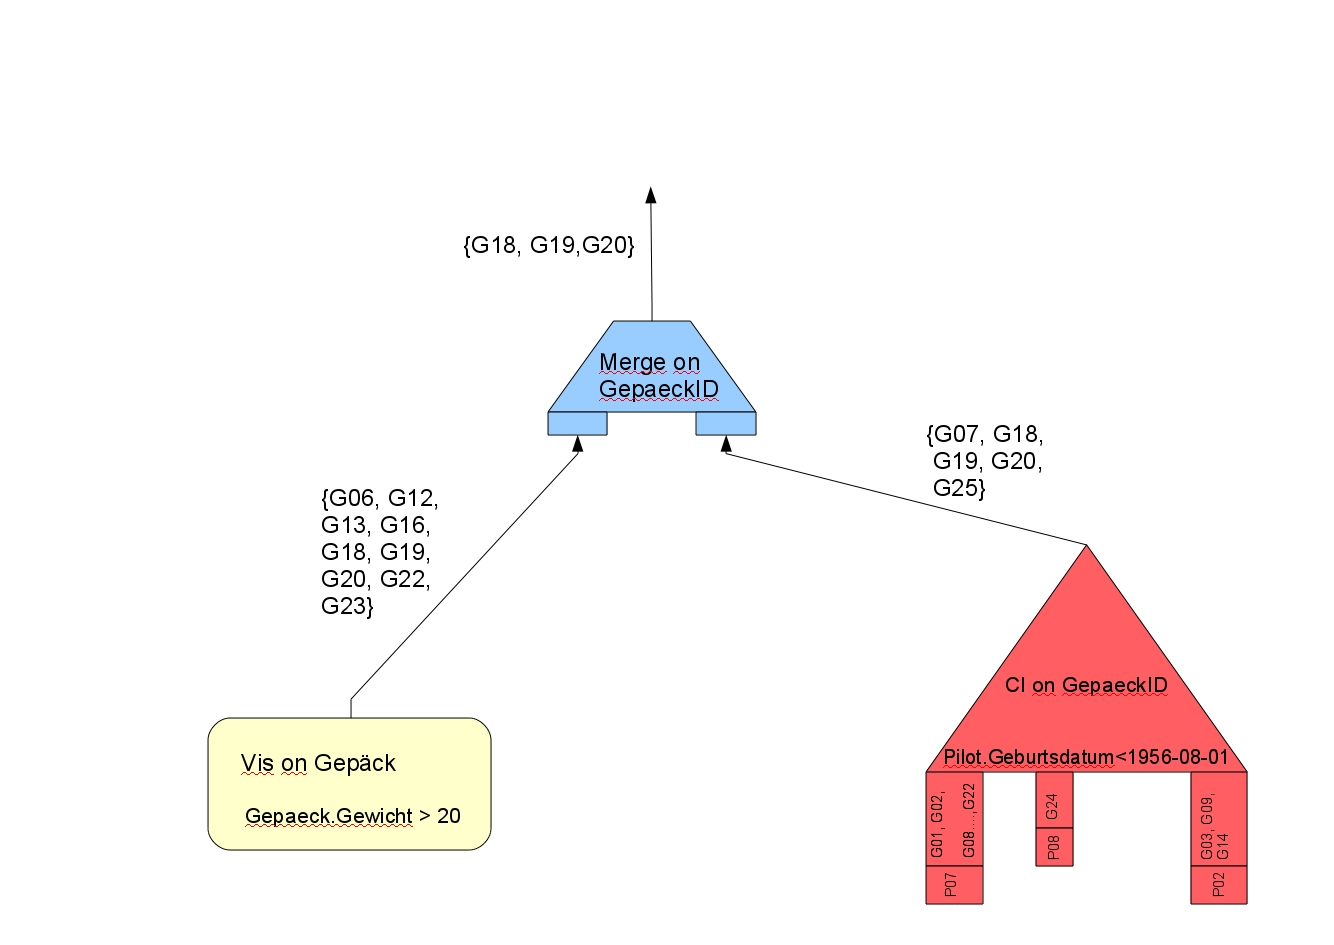
\includegraphics[trim = 0mm 10mm 0mm 20mm, clip, width=\textwidth]{img/Pre1}
  \caption{Teilergebnis Prefiltering 1}
  \label{fig:pre1}
\end{figure}

Von \textit{Piloten} aus wird analog der Weg �ber \textit{Buchungen} beschritten. ``Climbing Index'': \{\{\}, \{B08, B11, B18, B19, B20, B21\}, \{\}, \{\}\}, Merge: \{B08, B11, B18, B19, B20, B21\}.

\begin{figure}[H]
  \centering
  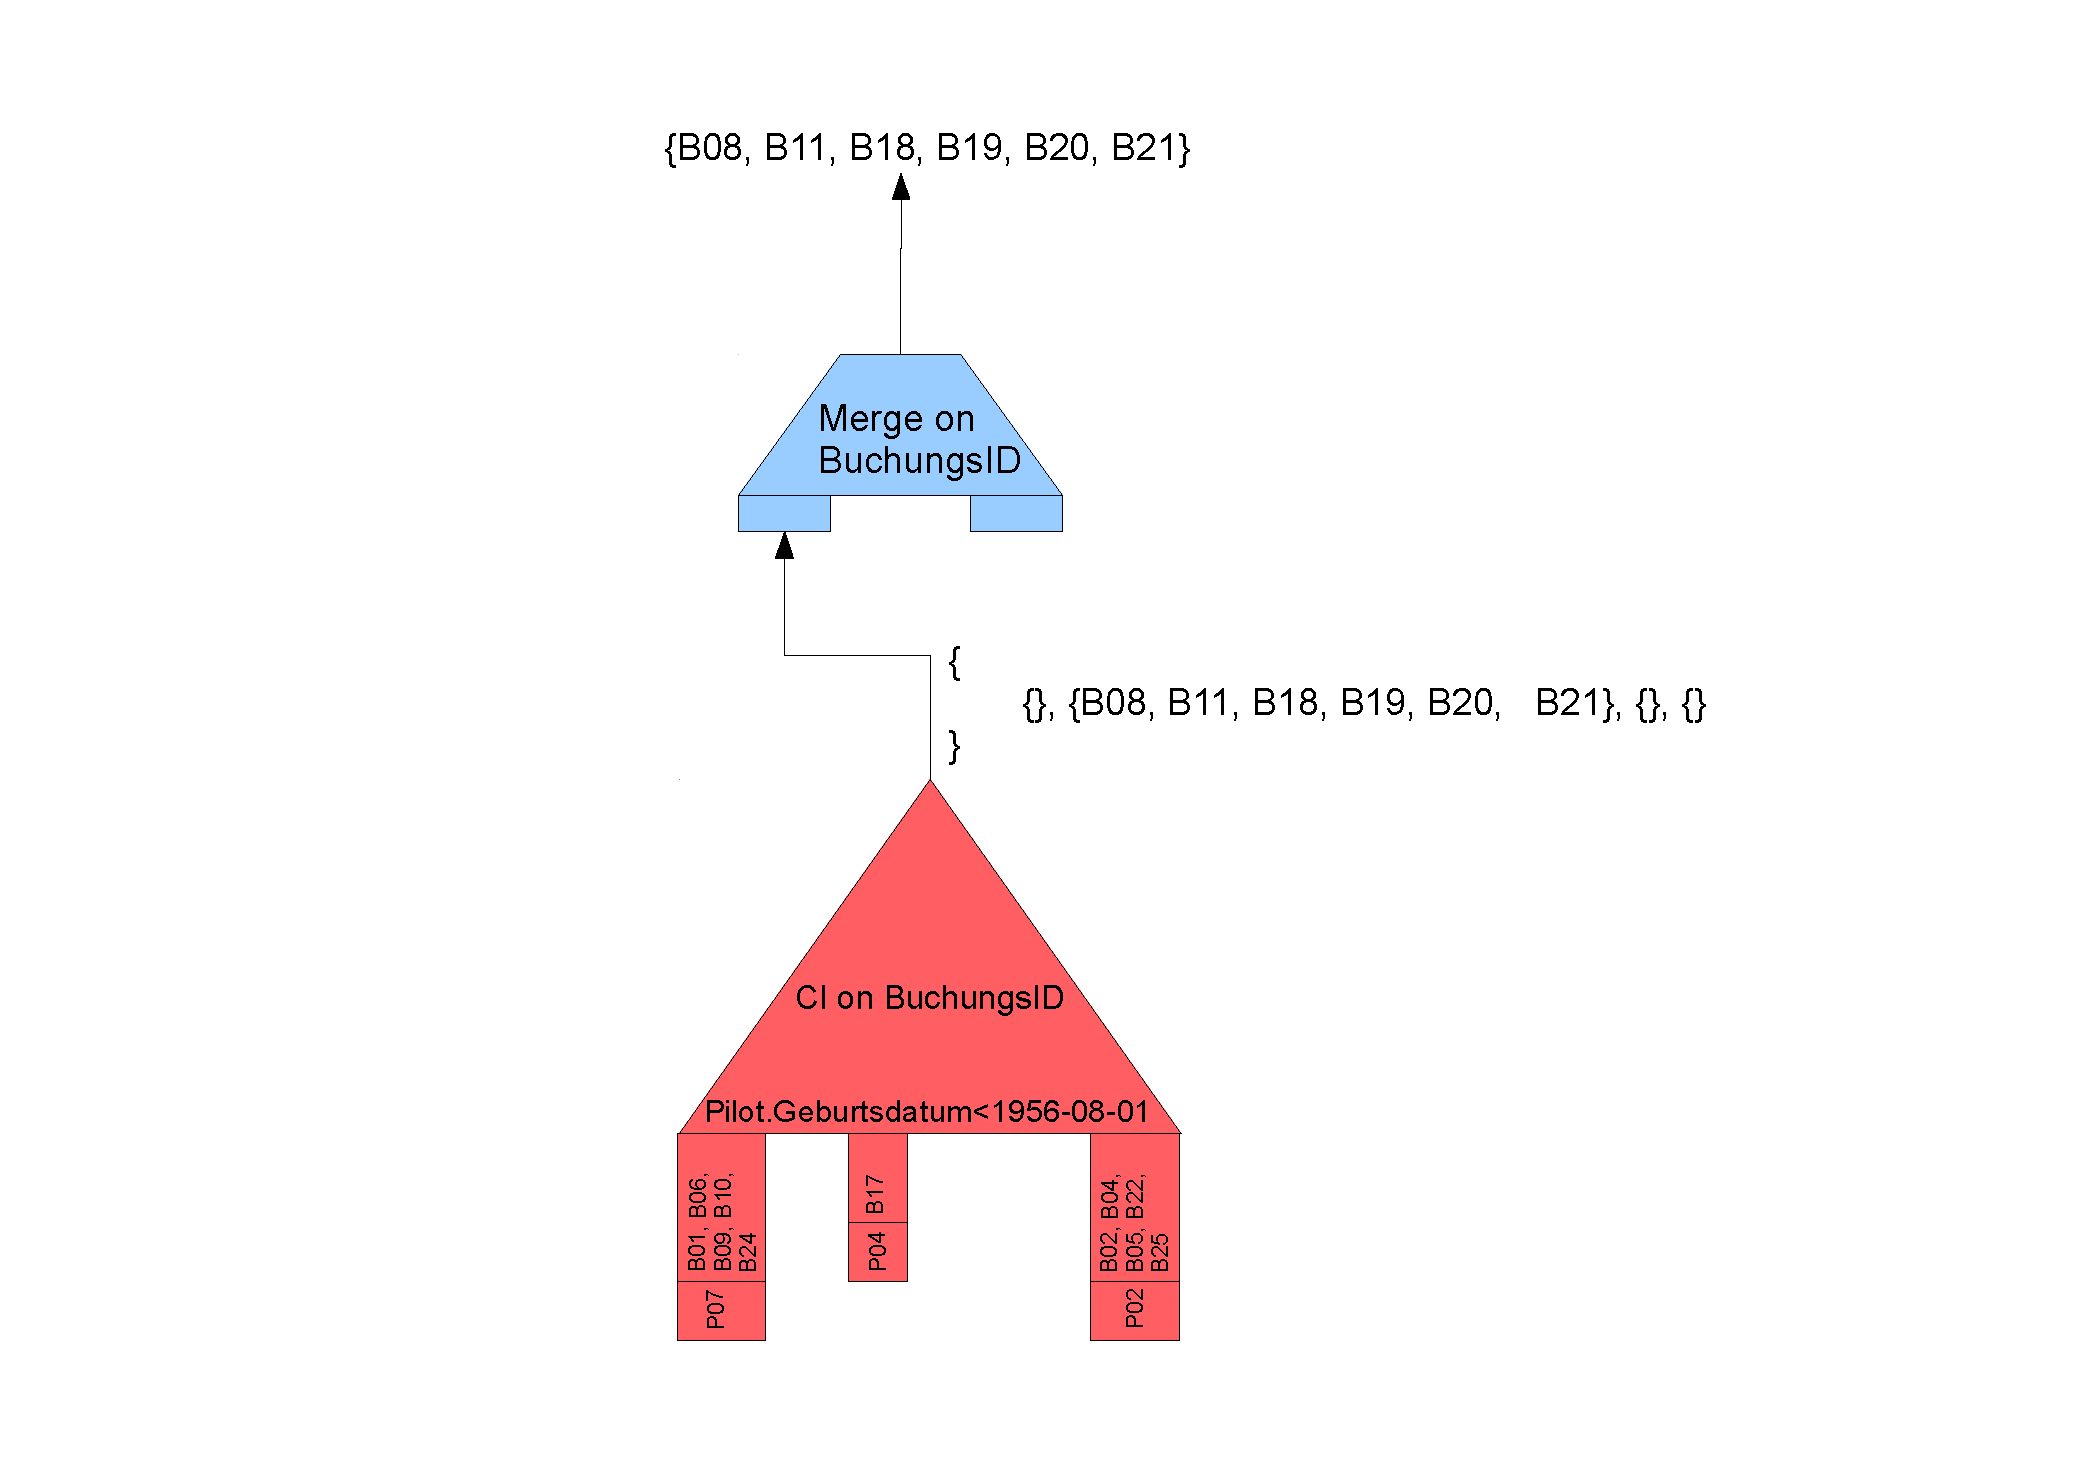
\includegraphics[trim = 0mm 20mm 0mm 10mm, clip, width=\textwidth]{img/Pre2.pdf}
  \caption{Teilergebnis Prefiltering 2}
  \label{fig:pre2}
\end{figure}

Unter Zuhilfenahme der entsprechenden ``Subtree Key Tables'' wird jeweils die Verbindung zur Tabelle \textit{Reisende} hergestellt: \{R07, R04, R04\} bzw. \{R07, R03, R13, R05, R04, R11\}. Mittels Merge wird der Durchschnitt beider Listen gebildet: \{R04, R07\}.

\begin{figure}[H]
  \centering
  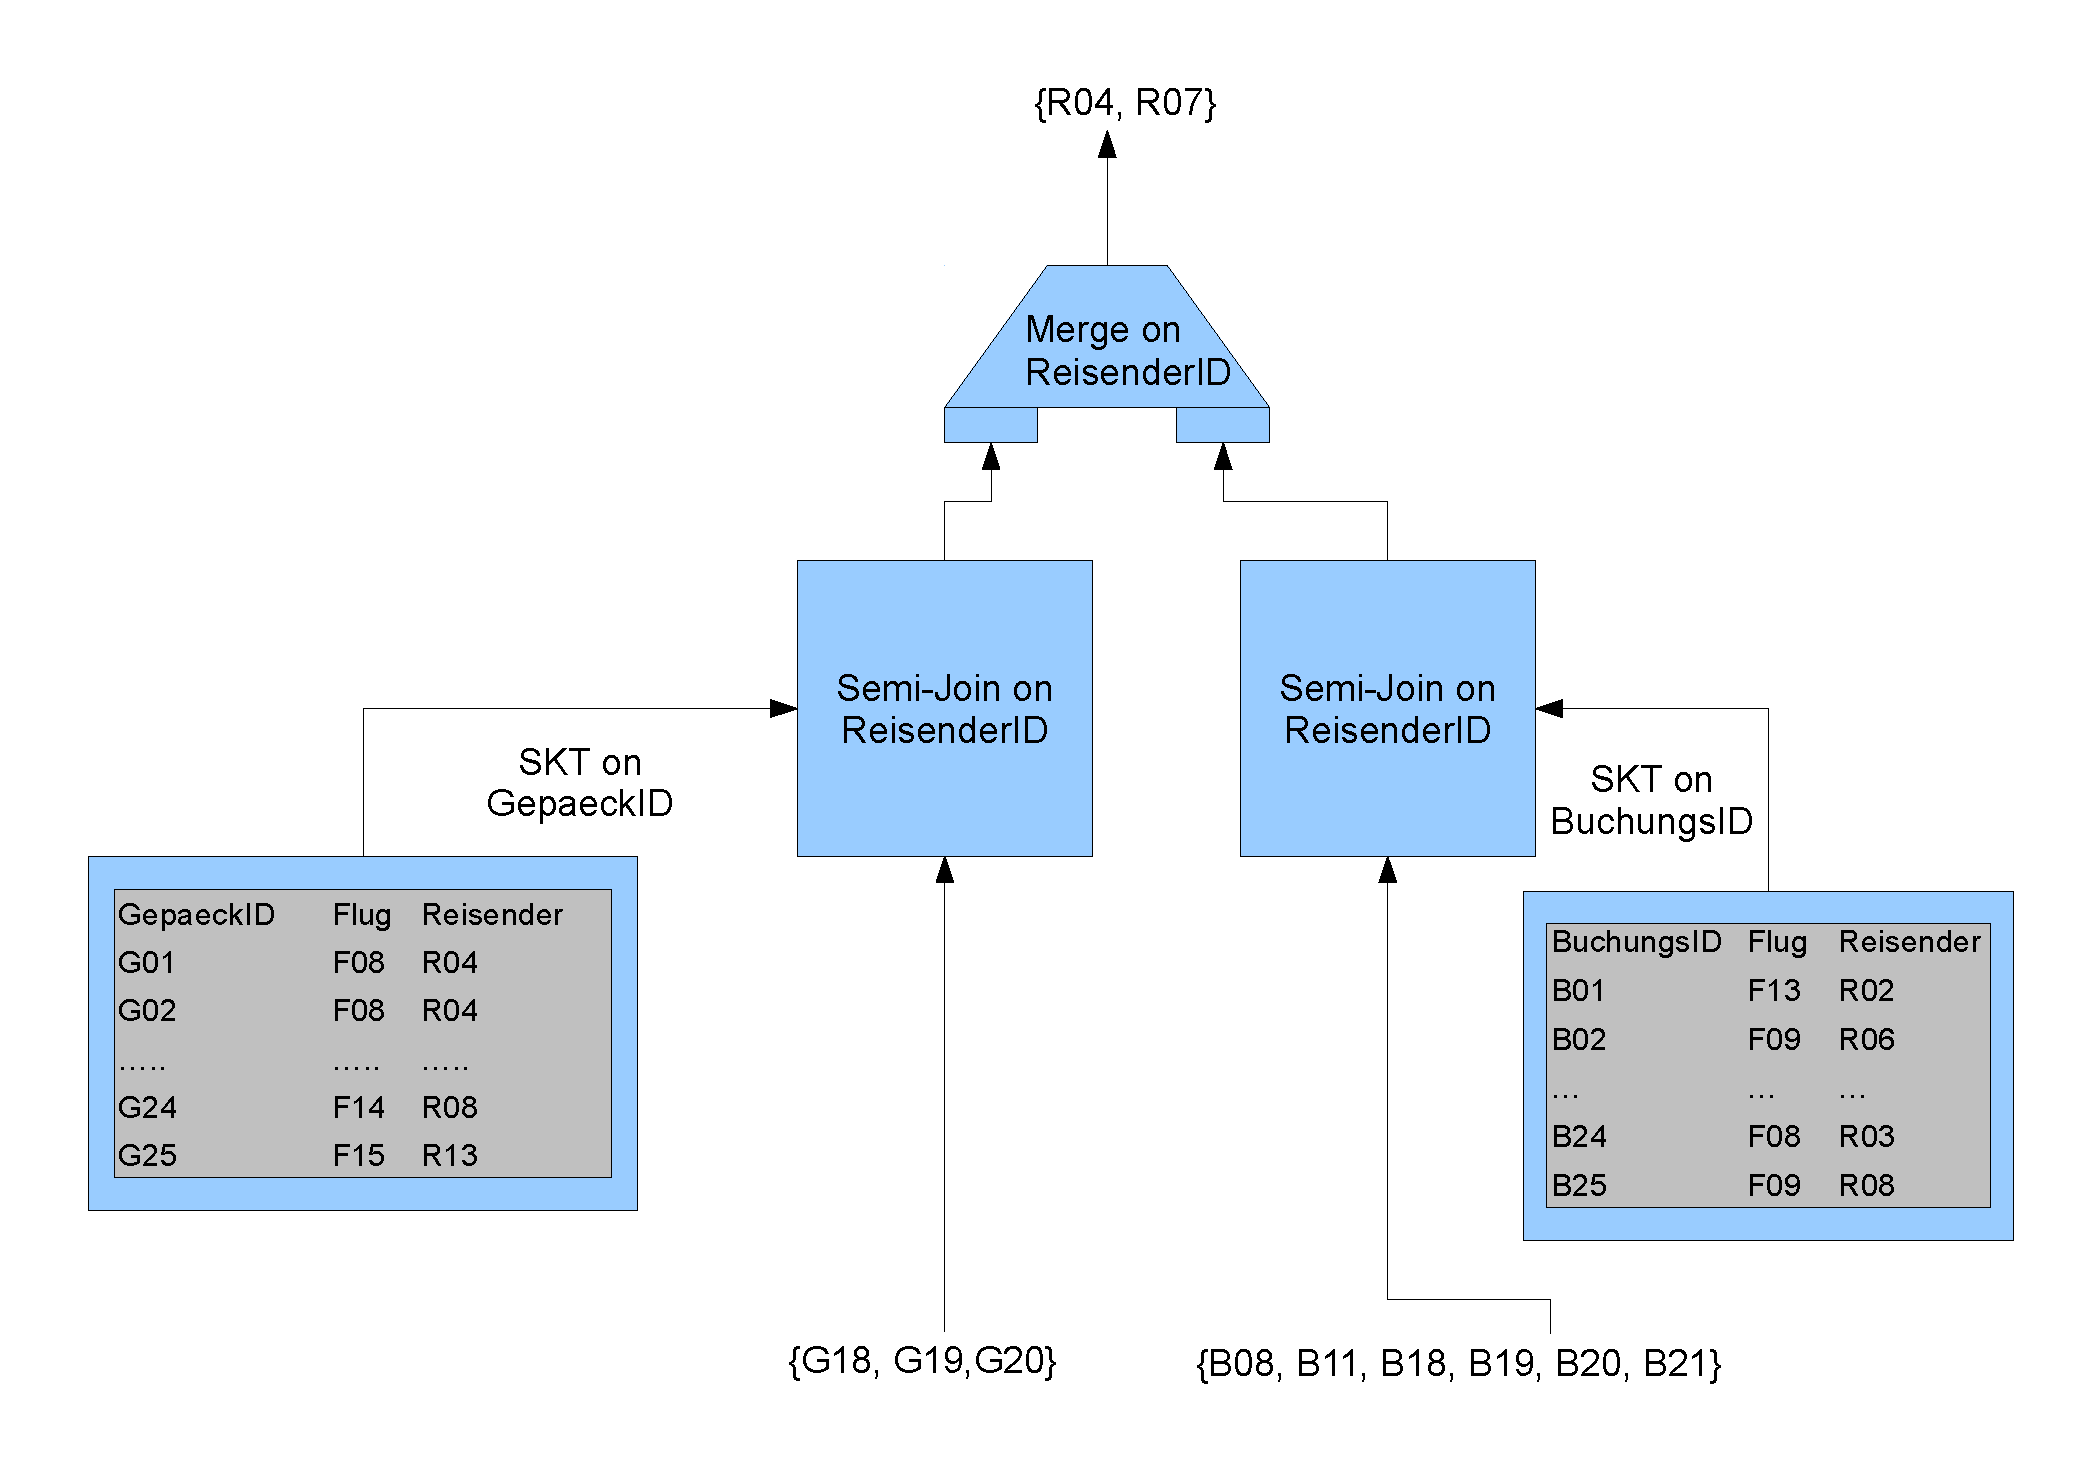
\includegraphics[trim = 0mm 10mm 0mm 0mm, clip, width=\textwidth]{img/Pre3.pdf}
  \caption{Teilergebnis Prefiltering 3}
  \label{fig:pre3}
\end{figure}

F�r die entstandene Liste wird ein Bloom-Filter erzeugt. Die noch ausstehende Selektion, R.Geschlecht='M', wird vom unsicheren Ger�t ausgef�hrt und das Ergbnis mittels Bloom-Filter gefiltert.

\begin{figure}[H]
  \centering
  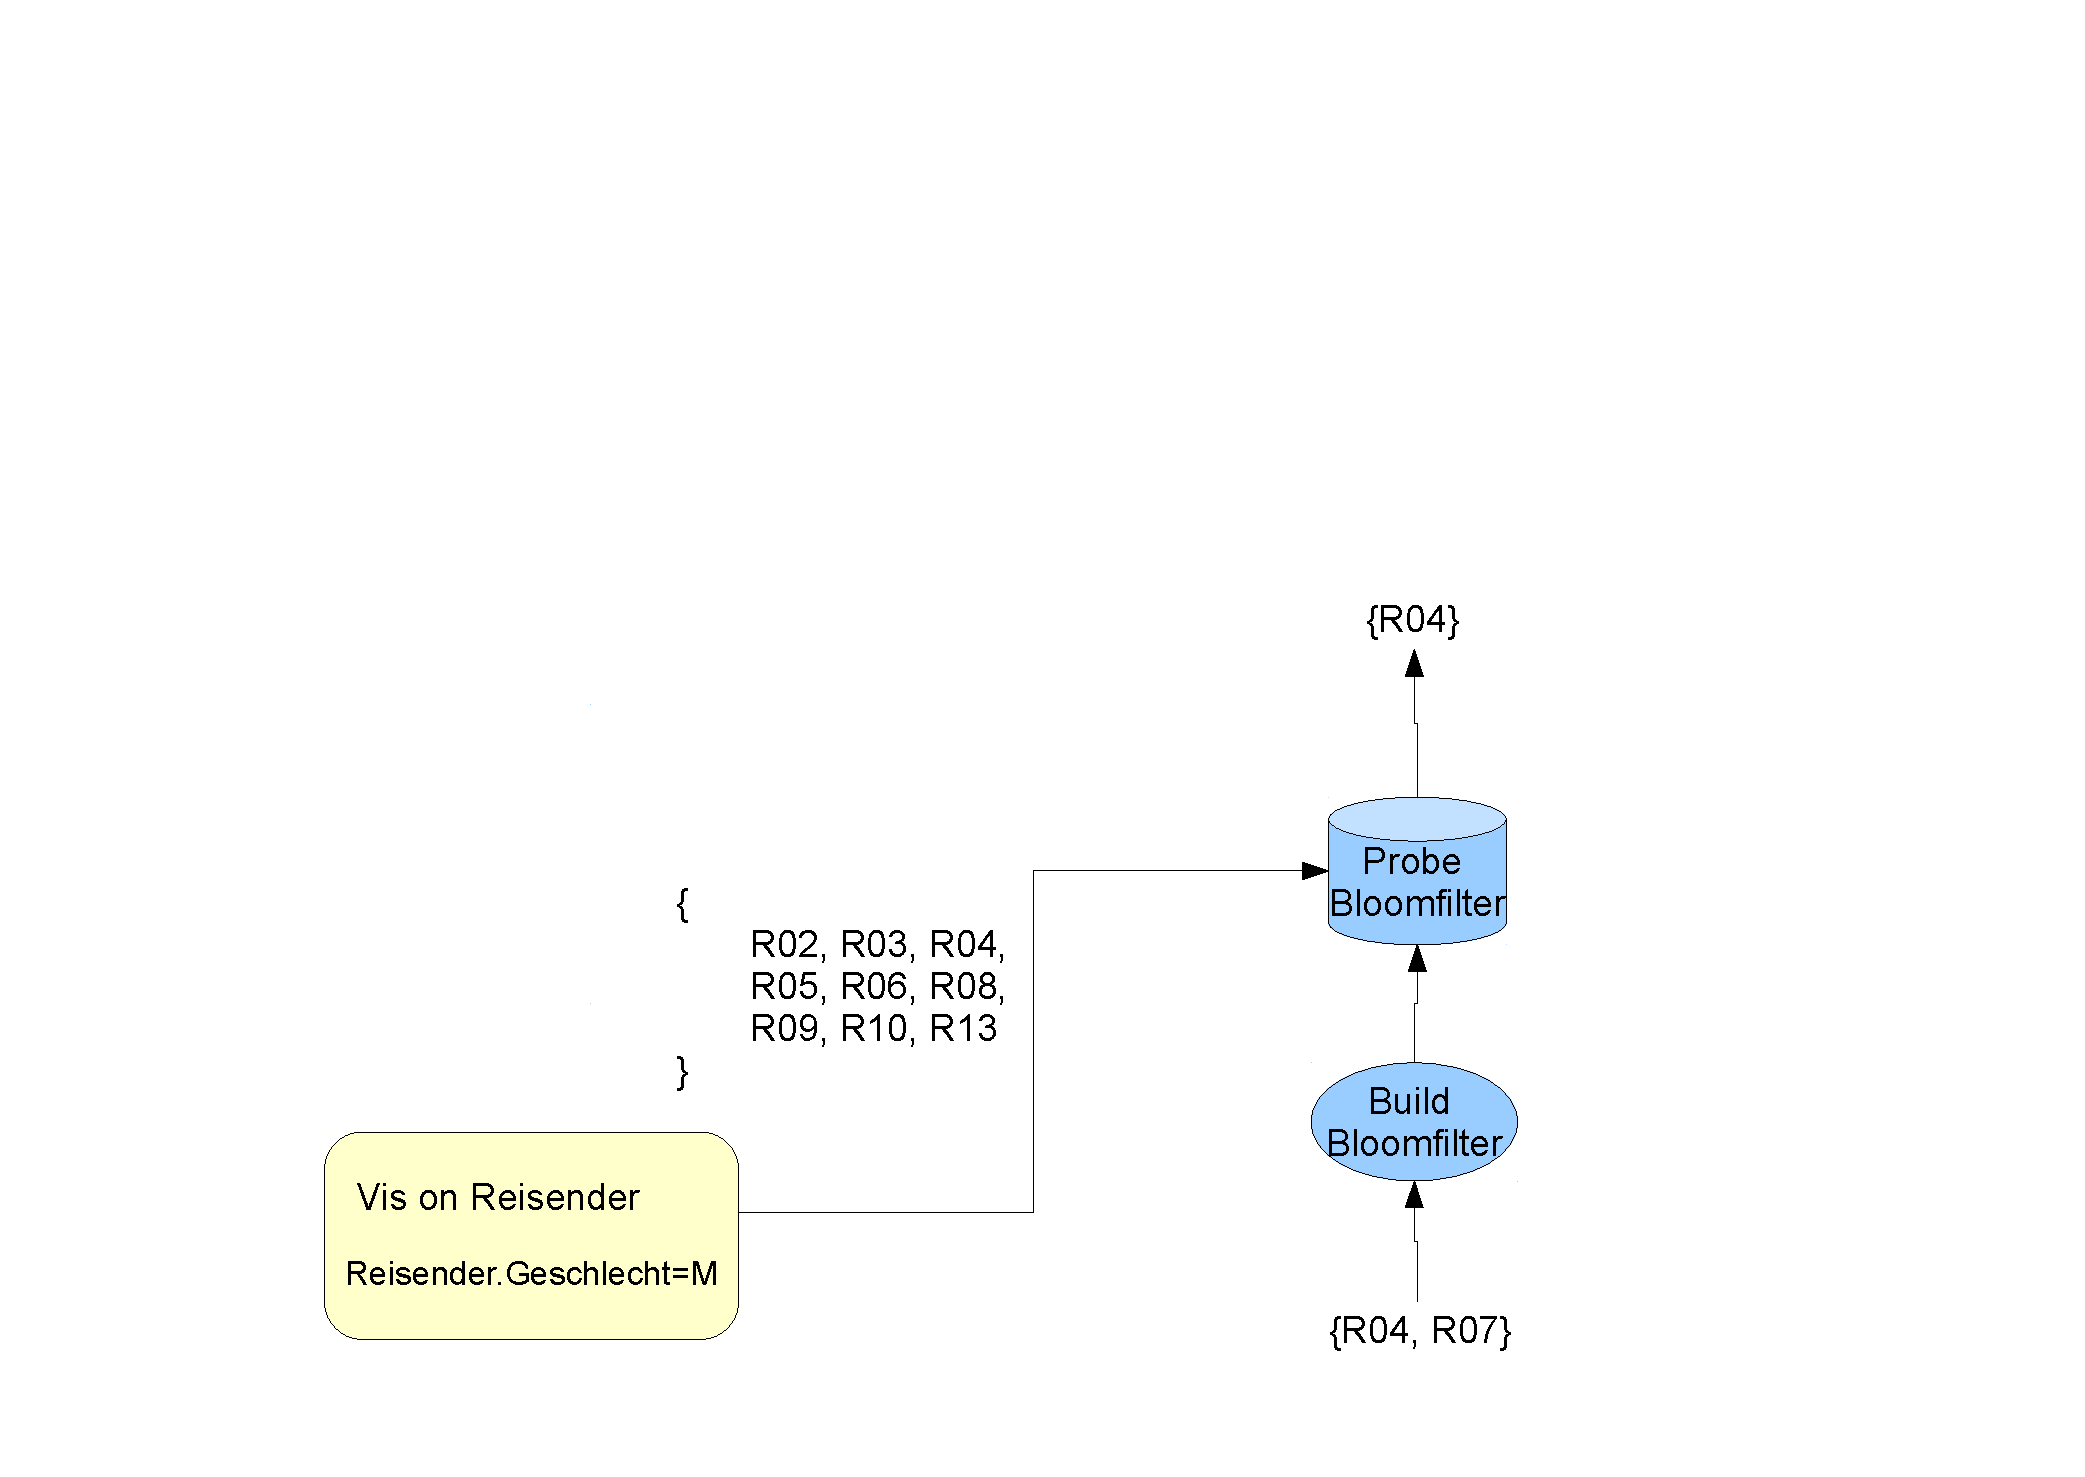
\includegraphics[trim = 0mm 20mm 0mm 80mm, clip, width=\textwidth]{img/Pre4.pdf}
  \caption{Teilergebnis Prefiltering 4}
  \label{fig:pre4}
\end{figure}

Mittels MJoin werden die noch verbleibenden Projektionen ausgef�hrt: \\\{$\langle$R04,Doru,Davidovici,Rom�nisch$\rangle$\}.

\begin{figure}[H]
  \centering
  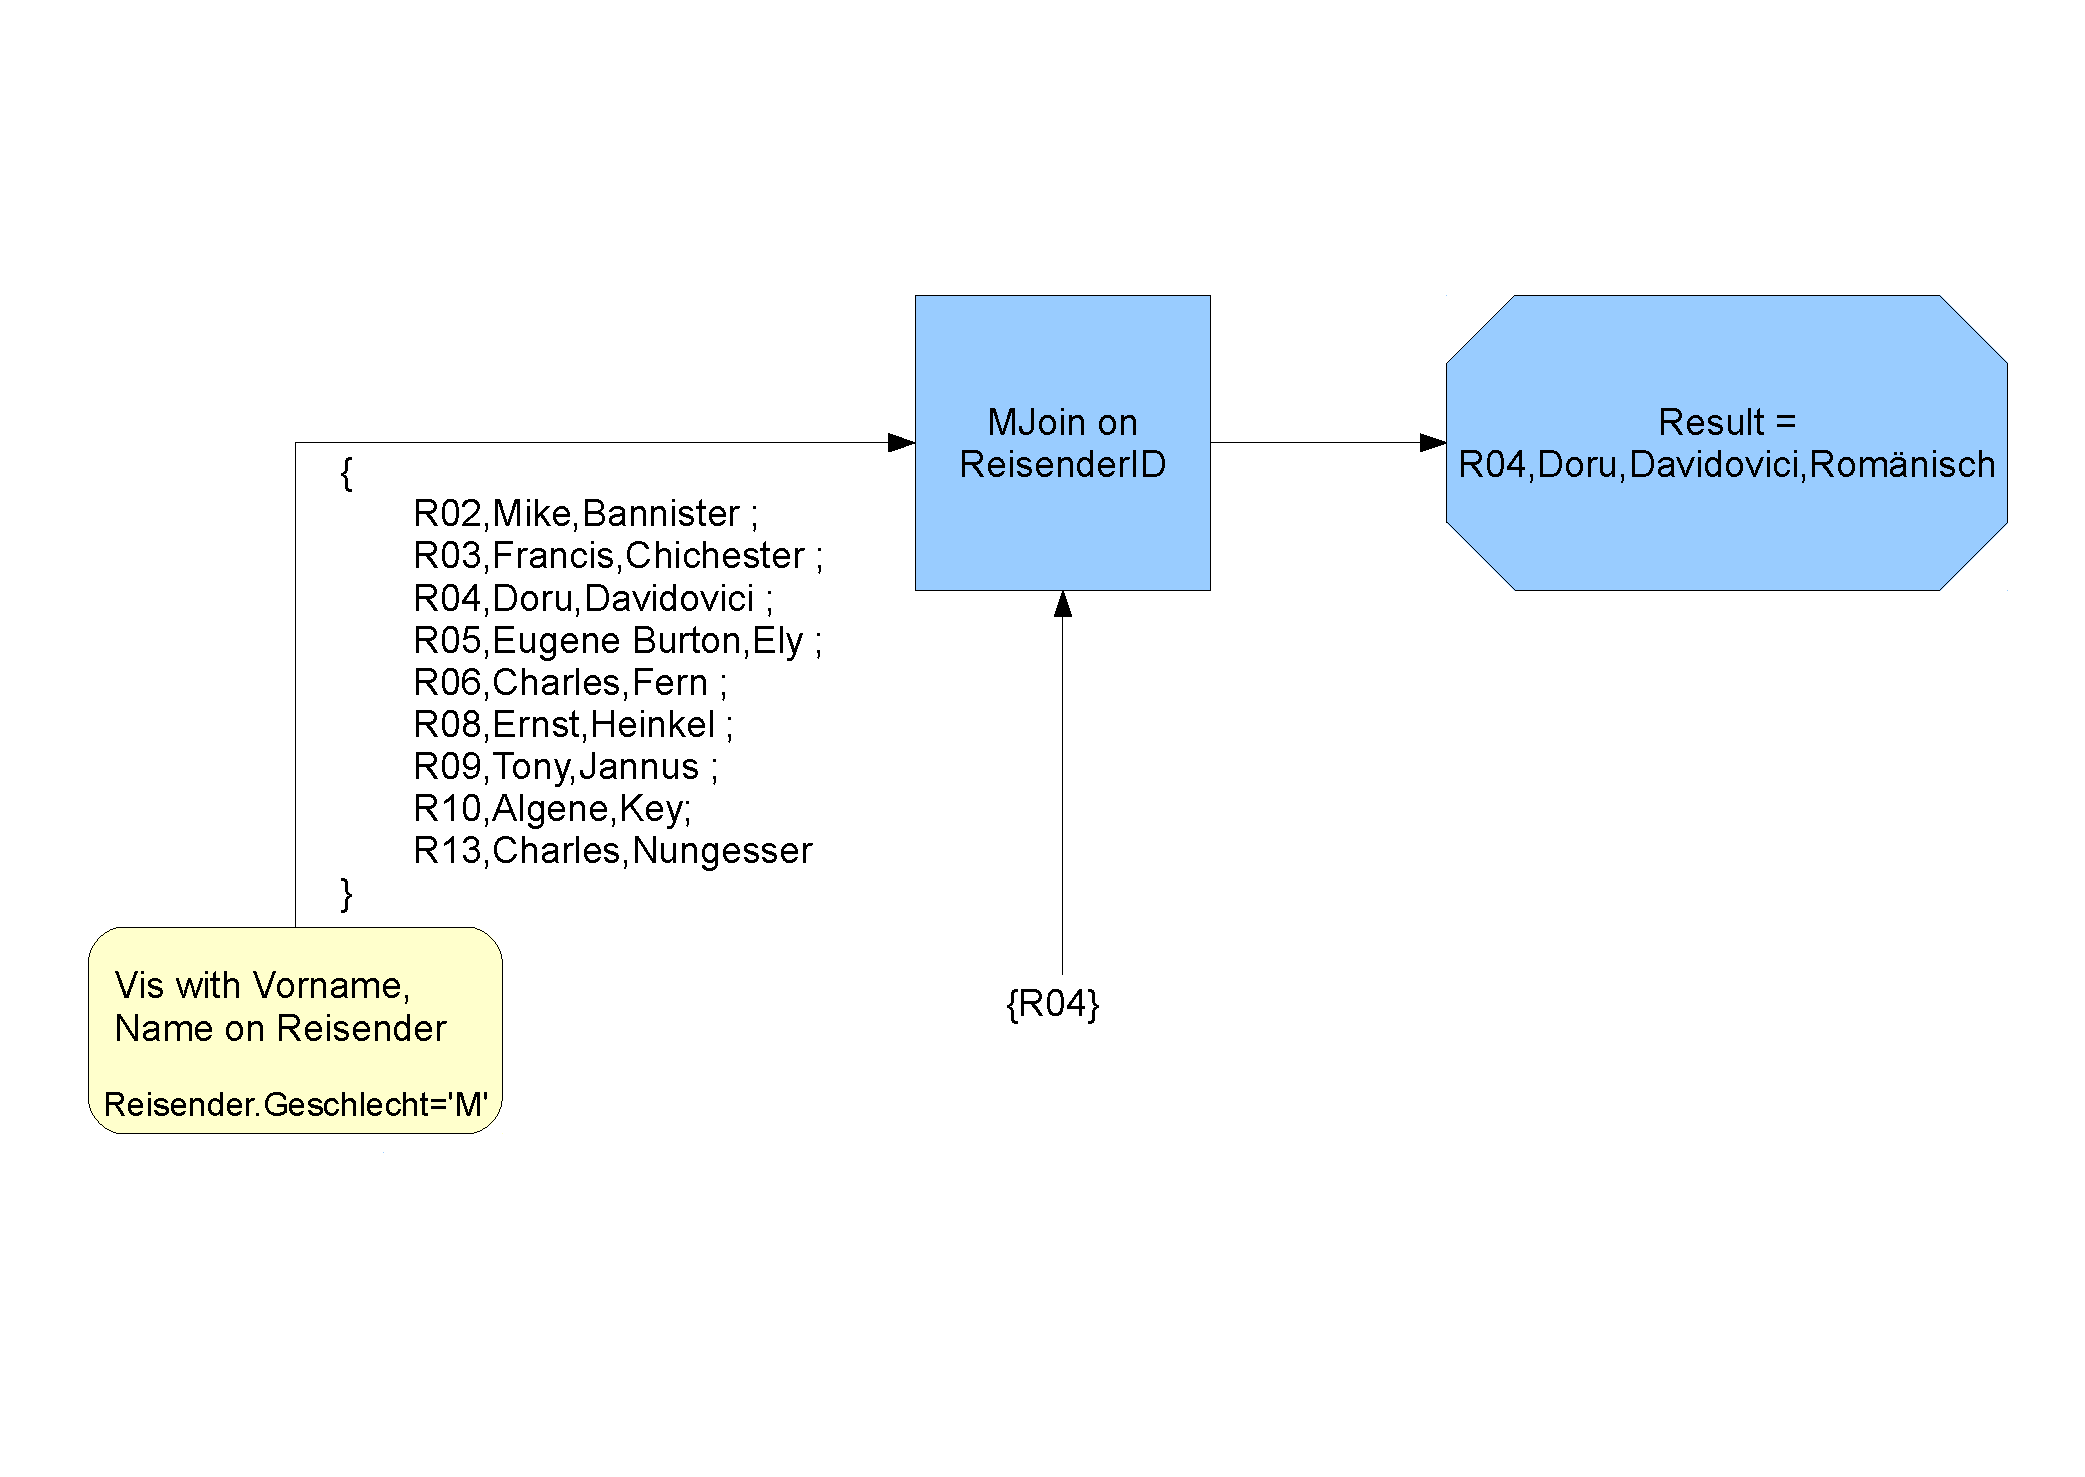
\includegraphics[trim = 0mm 80mm 0mm 20mm, clip, width=\textwidth]{img/Pre5.pdf}
  \caption{Teilergebnis Prefiltering 5}
  \label{fig:pre5}
\end{figure}

F�gt man die einzelnen Schritte zusammen, entsteht folgender Ausf�hrungsplan f�r das ``Prefiltering'':

\begin{figure}[H]
  \centering
  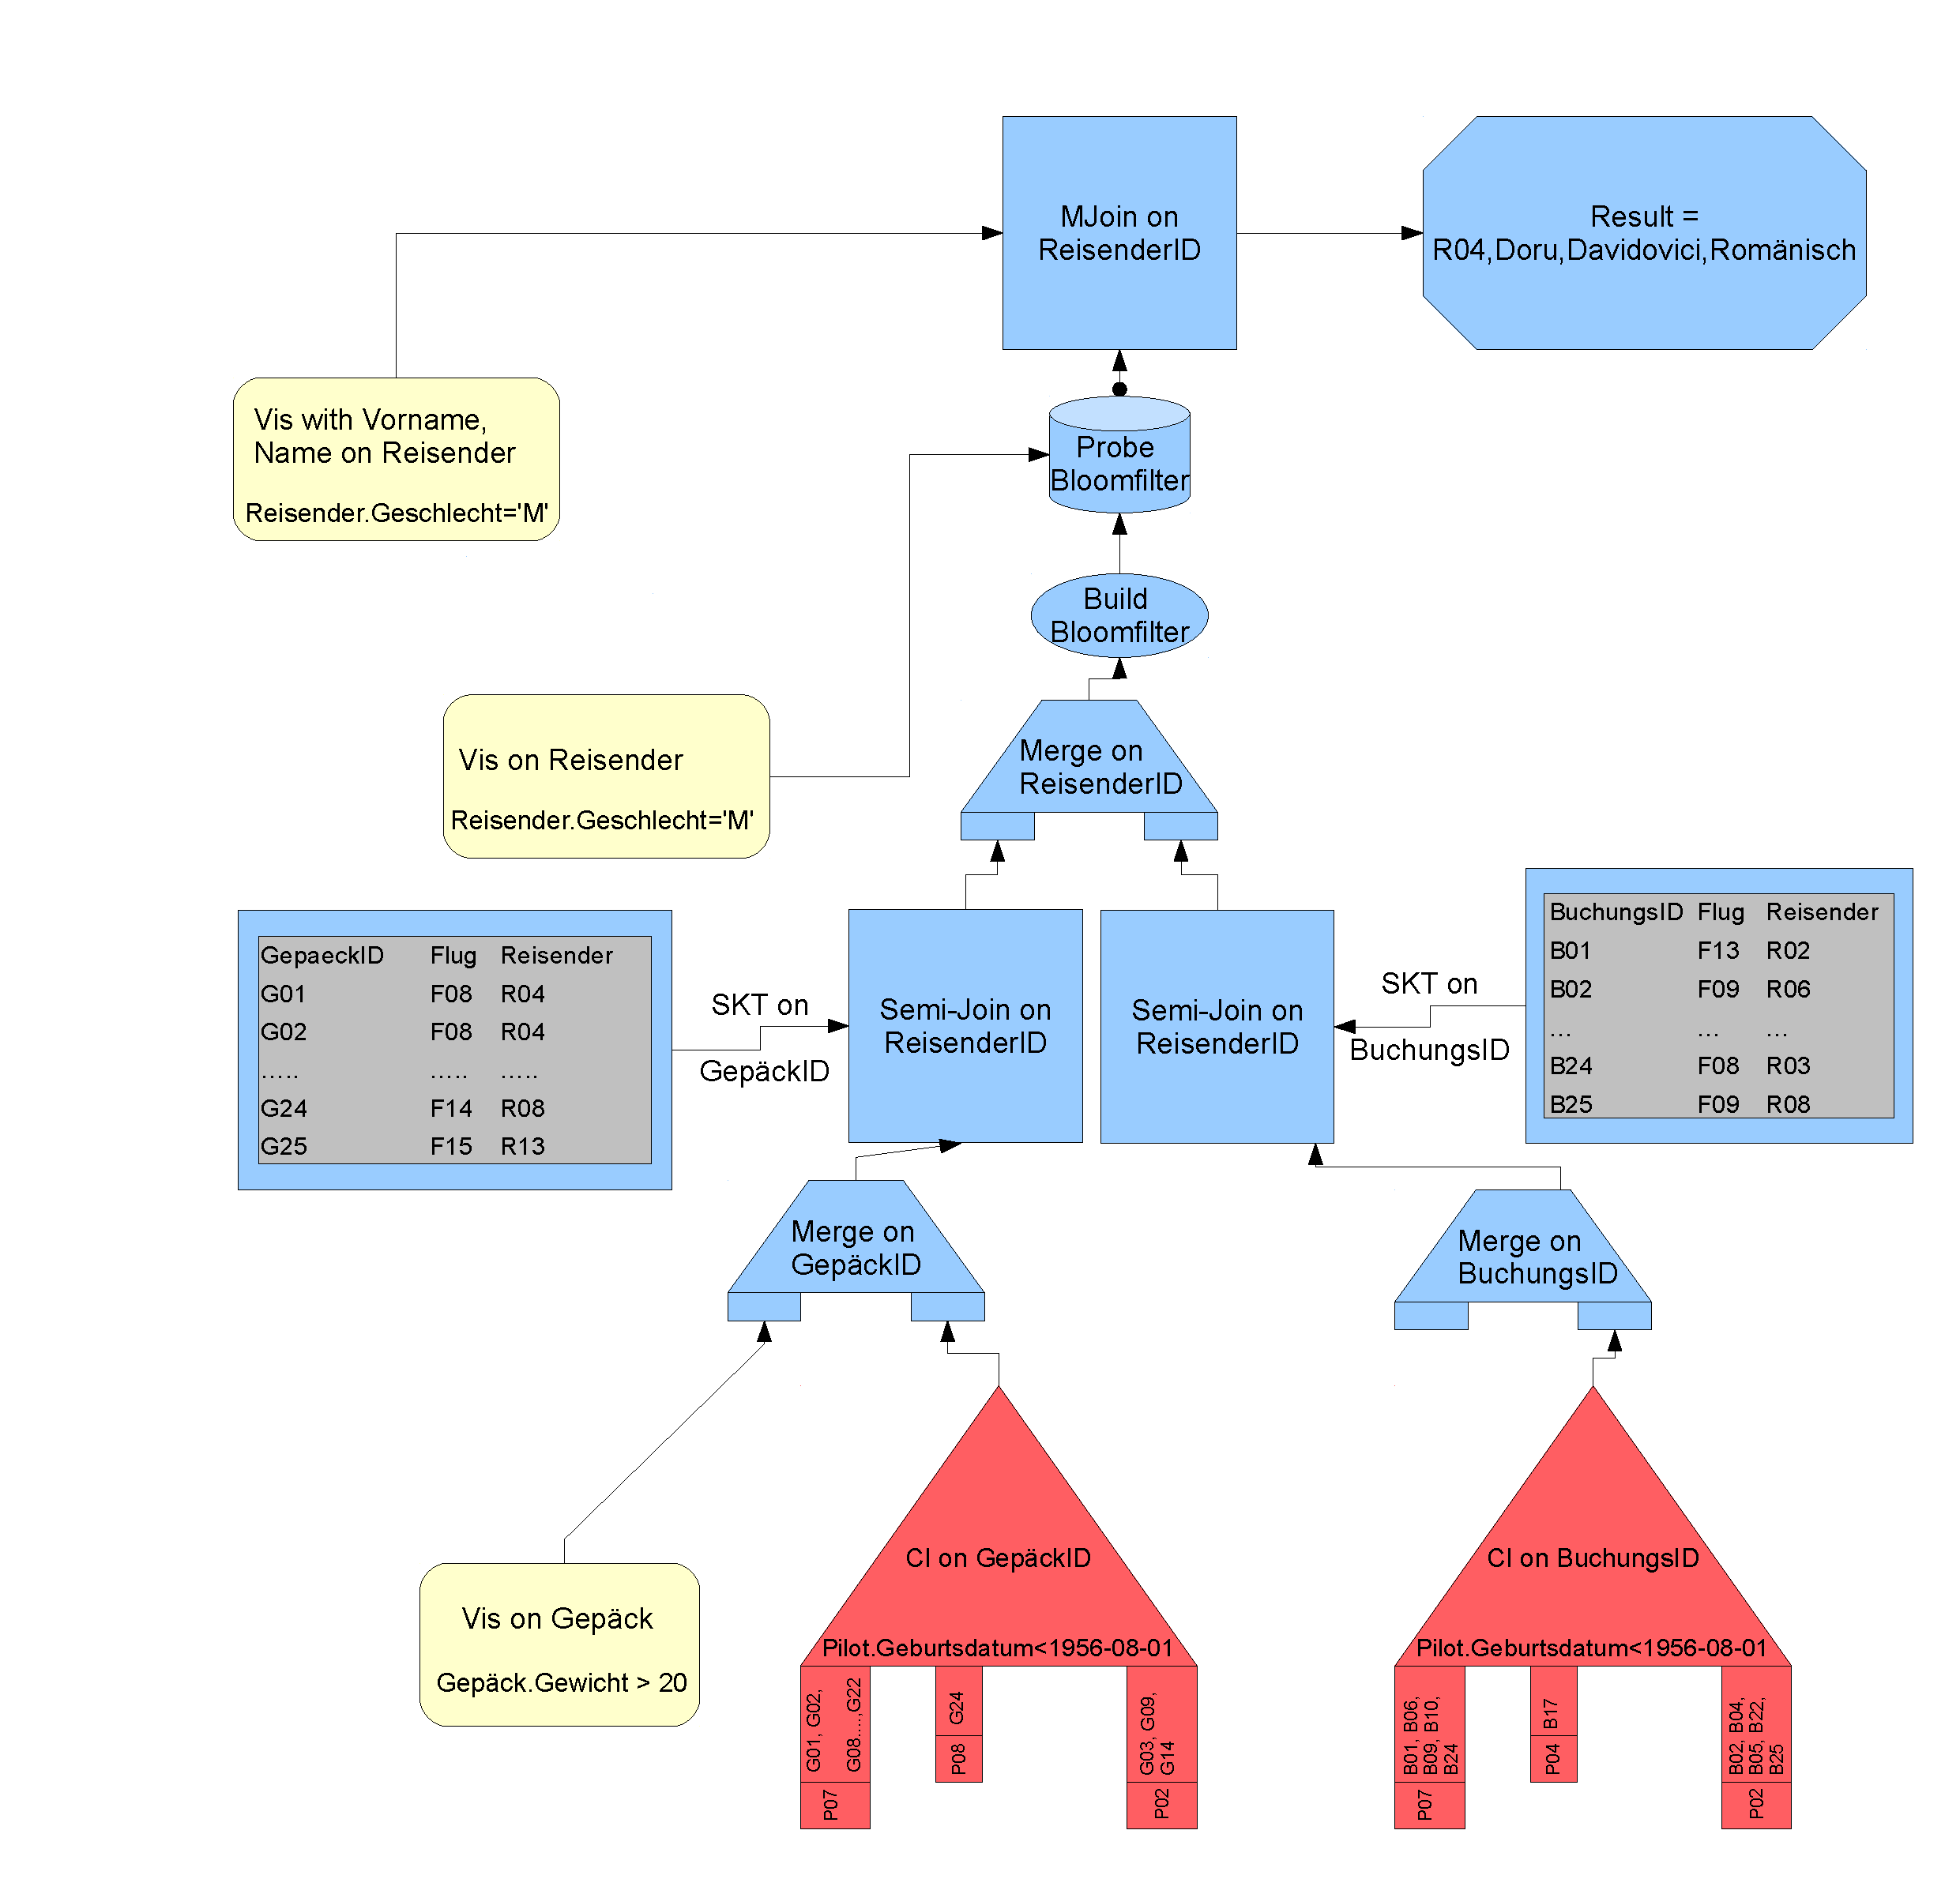
\includegraphics[trim = 0mm 20mm 0mm 0mm, clip, width=\textwidth]{img/Pre-Filtering.pdf}
  \caption{Prefiltering QEP}
  \label{fig:pre}
\end{figure}

Unter Verwendung der in \cite{ghostdb1} definierten Operanden, l�sst sich der ``Prefiltering'' Plan auch wie folgt aufschreiben:

\begin{enumerate}[1]
\item Vis(Q,Gepaeck,G.GepaeckID) = \{G06, G12, G13, G16, G18, G19, G20, G22, G23\}
\item CI(P.Geburtsdatum,<1956-08-01,G.GepaeckID) = \{\{\}, \{G07, G18, G19, G20, G25\}, \{\}, \{\}\}
\item Merge(($\bigcup 2)\cap 1$) = \{G18, G19, G20\}
\item SJoin(3,$\text{SKT}_{\text{Gepaeck}}$,R.ReisenderID) = \{R07, R04, R04\}
\item CI(P.Geburtsdatum,<1956-08-01,B.BuchungsID) = \{\{\}, \{B08, B11, B18, B19, B20, B21\}, \{\}, \{\}\}
\item Merge($\bigcup 5$) = \{B08, B11, B18, B19, B20, B21\}
\item SJoin(6,$\text{SKT}_{\text{Buchungen}}$,R.ReisenderID) = \{R07, R03, R13, R05, R04, R11\}
\item Merge($4\cap 7$) = \{R04, R07\}
\item BuildBF(8) = BF
\item Vis(Q,Reisende,R.ReisenderID) = \{R02, R03, R04, R05, R06, R08, R09, R10, R13\}
\item ProbeBF(BF,10) = \{R04\}
\item Vis(Q,Reisende,$\langle$R.ReisenderID,R.Vorname,R.Name$\rangle$) = \{$\langle$R02,Mike,Bannister$\rangle$, \\
$\langle$R03,Francis,Chichester$\rangle$, $\langle$R04,Doru,Davidovici$\rangle$, $\langle$R05,Eugene Burton,Ely$\rangle$, \\$\langle$R06,Charles,Fern$\rangle$, $\langle$R08,Ernst,Heinkel$\rangle$, $\langle$R09,Tony,Jannus$\rangle$, $\langle$R10,Algene,Key$\rangle$, \\$\langle$R13,Charles,Nungesser$\rangle$\}
\item MJoin(12,11,$\langle$R.ReisenderID,R.Staatsbuergerschaft$\rangle$,8) = \\\{$\langle$R04,Doru,Davidovici,Rom�nisch$\rangle$\}
\end{enumerate}

Das Problem an dieser Strategie ist allerdings, dass bei zu geringer Selektivit�t der sichtbaren Selektionen zu wenige Tupel im Vorfeld aussortiert werden und somit ein gro�er Vorteil des ``Prefilterings'' verschwindet. Eine Alternative, die diesem Effekt entgegen wirkt ist das ``Postfiltering''.

\section{Postfiltering}
Beim ``Postfiltering'' werden zuerst alle Selektionen ausgef�hrt und mittels Joins zusammengefasst, die auf den sicheren Bereich zugreifen. Erst danach werden unter Verwendung von Bloom-Filtern die Selektionen des unsicheren Bereiches hinzugef�gt.

F�r unser Beispiel hei�t dies, dass zuerst die Selektion auf dem Geburtsdatum des Piloten ausgef�hrt wird. Es wird der ``Climbing Index'' verwendet, um \textit{GepackIDs} zu erhalten: \{\{\}, \{G07, G18, G19, G20, G25\}, \{\}, \{\}\}.

\begin{figure}[H]
  \centering
  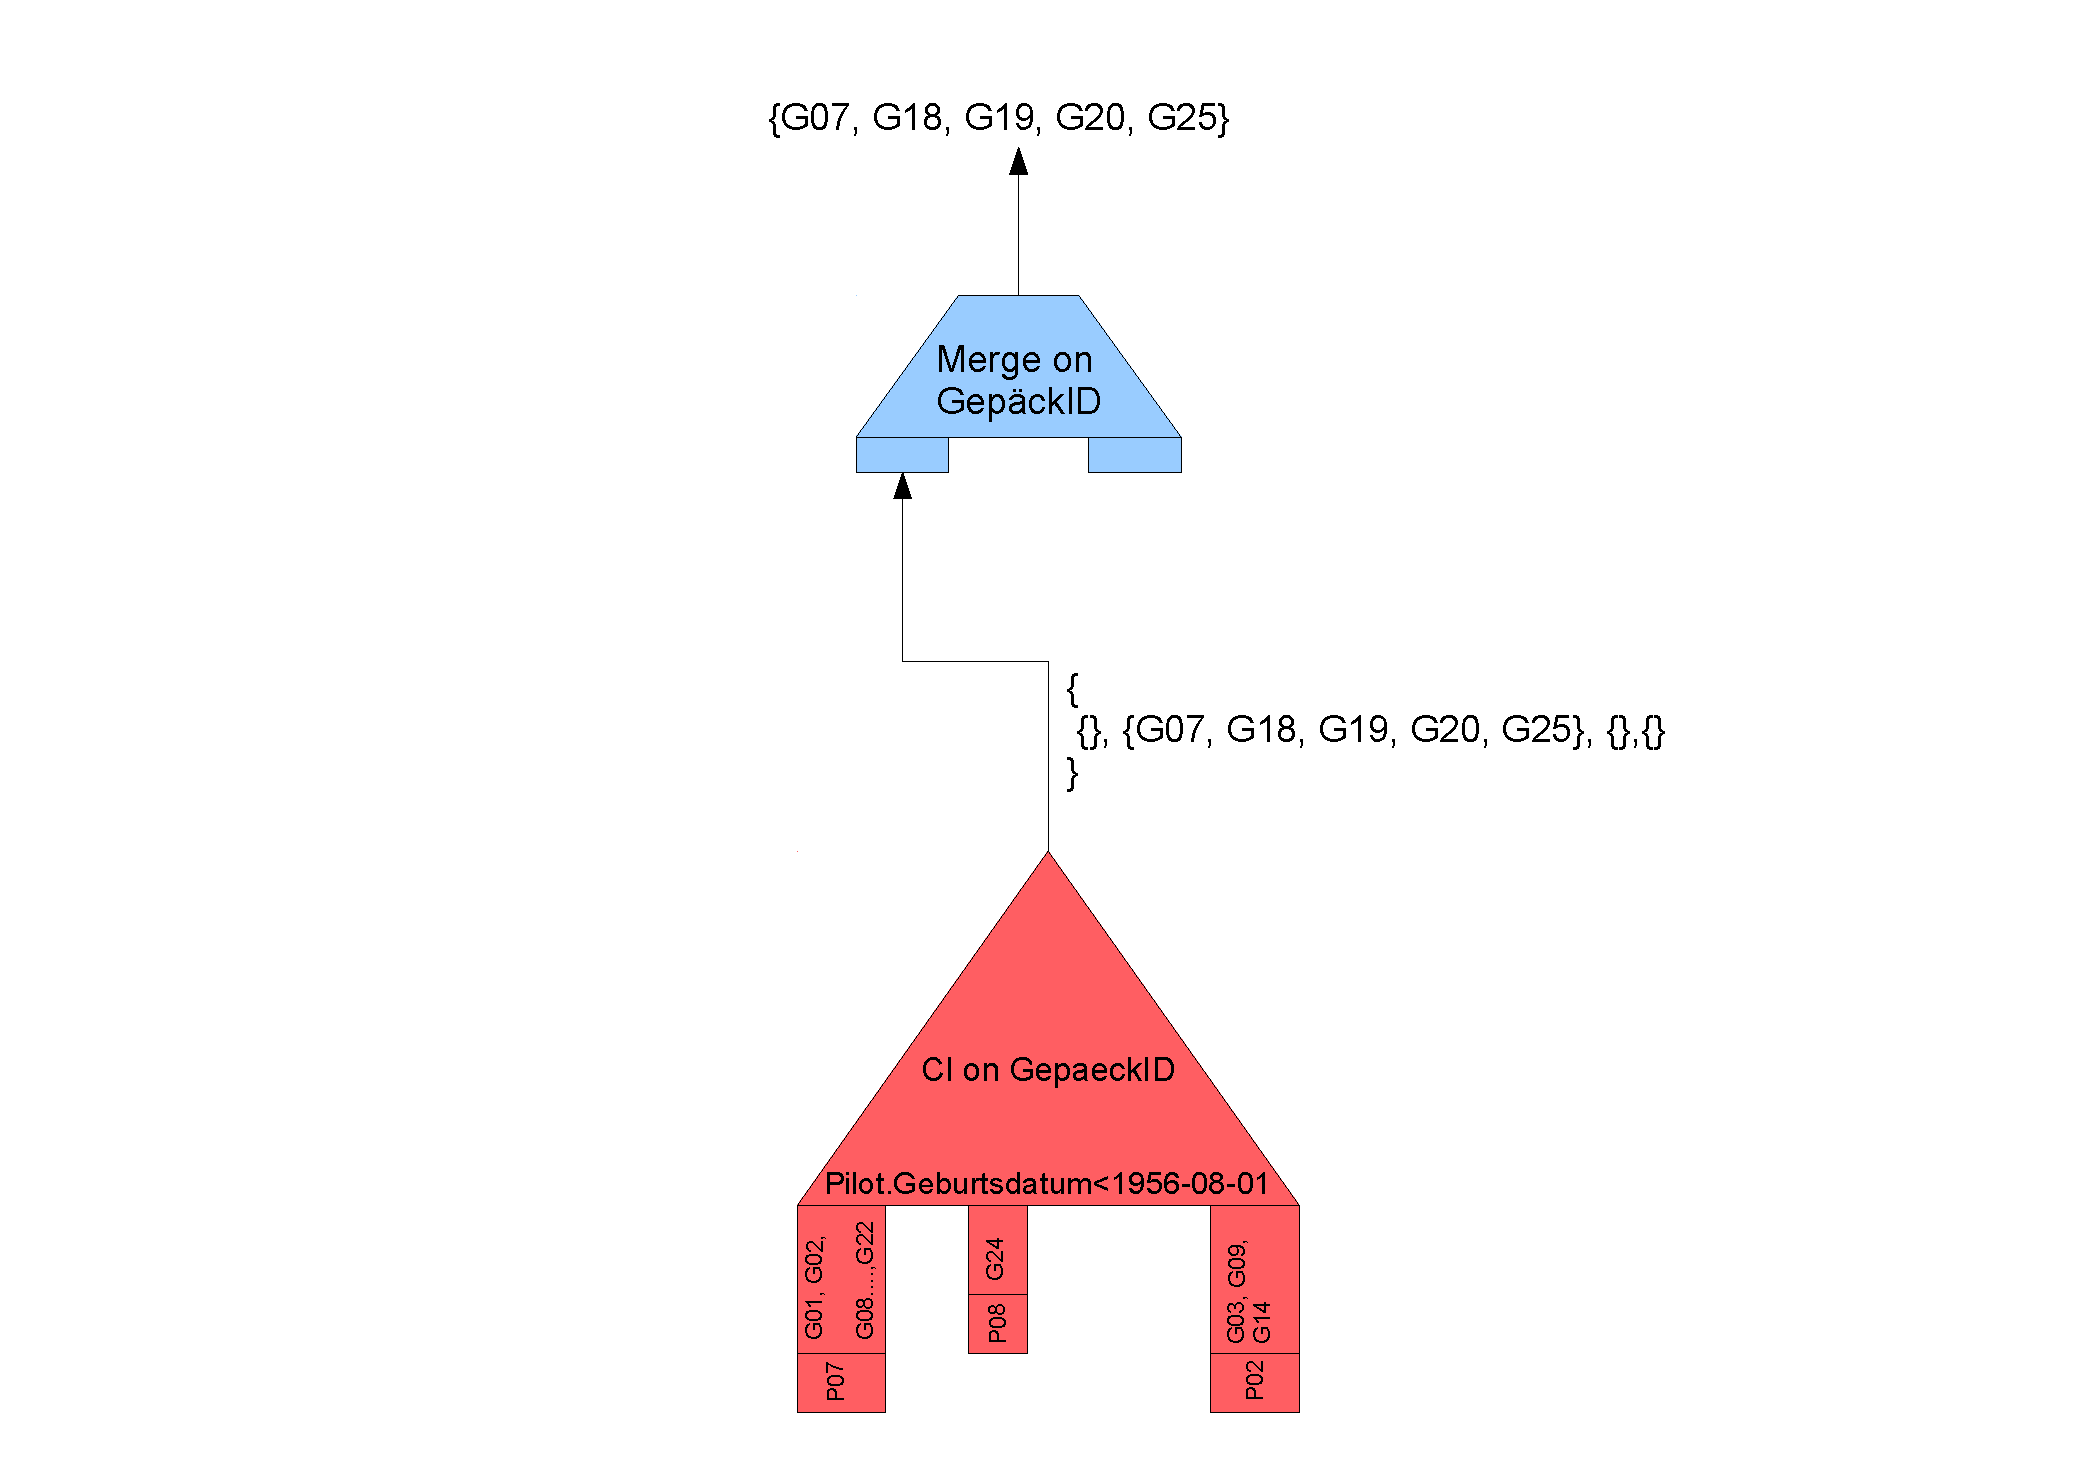
\includegraphics[trim = 0mm 20mm 0mm 10mm, clip, width=\textwidth]{img/Post1.pdf}
  \caption{Teilergebnis Postfiltering 1}
  \label{fig:post1}
\end{figure}

Anschlie�end wird ein ``Subtree Key Table'' genutzt, um passende \textit{ReisenderIDs} zu berechnen: \{$\langle$G07,R11$\rangle$, $\langle$G18,R07$\rangle$, $\langle$G19,R04$\rangle$, $\langle$G20,R04$\rangle$, $\langle$G25,R13$\rangle$\}

\begin{figure}[H]
  \centering
  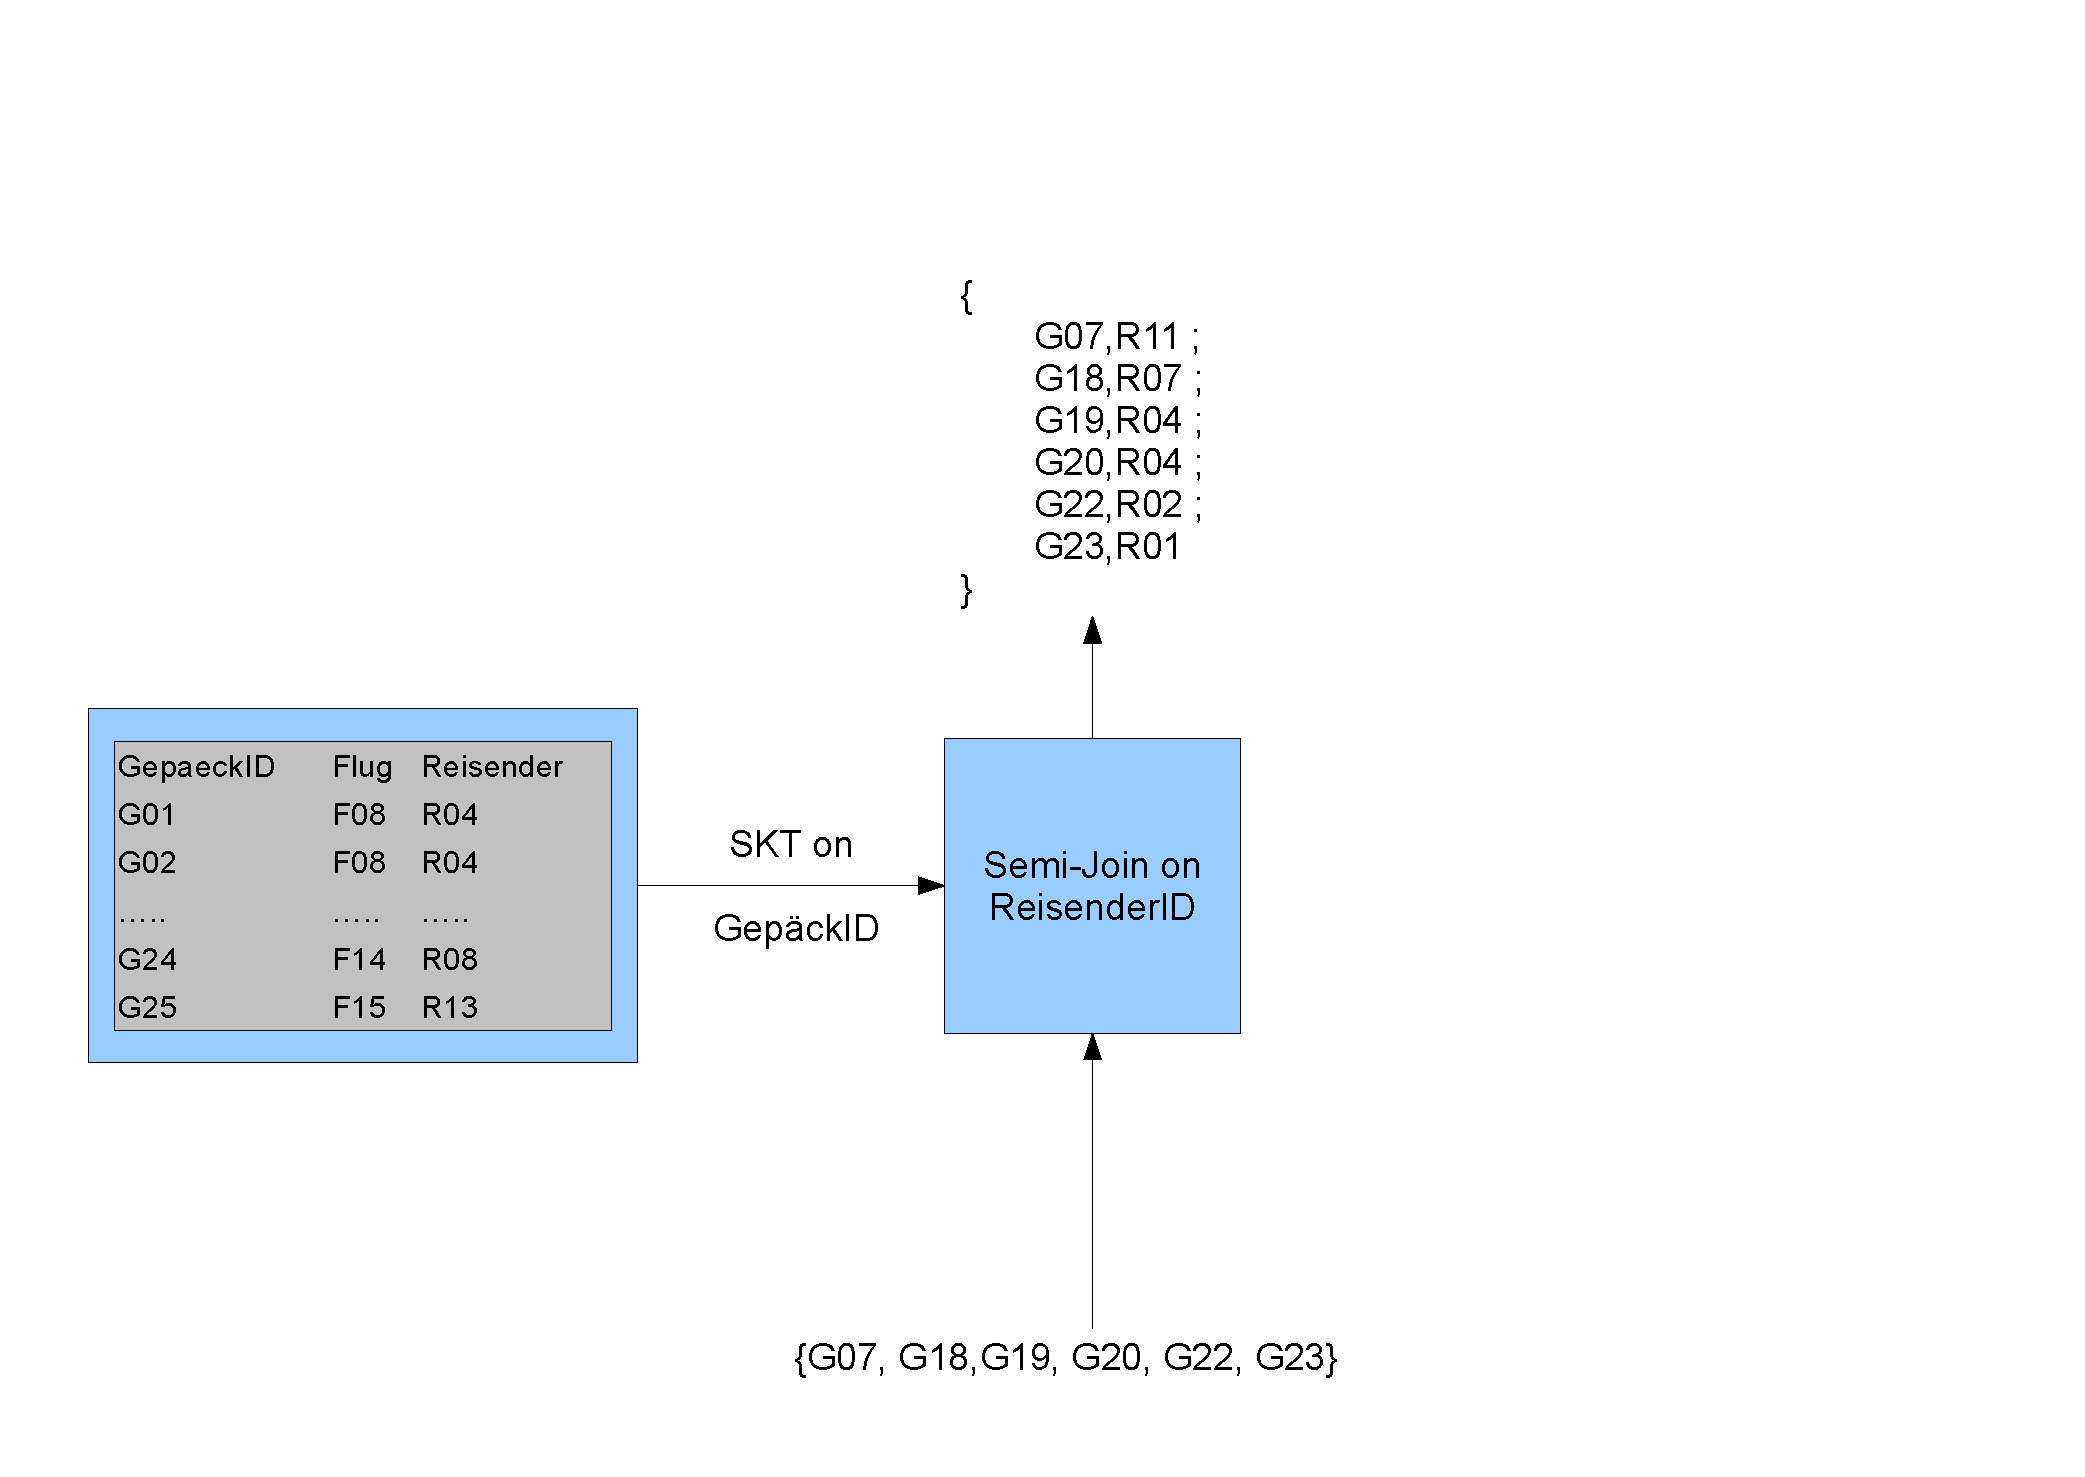
\includegraphics[trim = 0mm 10mm 0mm 40mm, clip, width=\textwidth]{img/Post2.pdf}
  \caption{Teilergebnis Postfiltering 2}
  \label{fig:post2}
\end{figure}

Das unsichere Ger�t liefert die Gep�ckst�cke, die schwerer als 20 Kilogramm sind. Es wird ein Bloom-Filter erzeugt und auf das vorhandene Zwischenergebnis angewendet: \{$\langle$G18,R07$\rangle$, $\langle$G19,R04$\rangle$, $\langle$G20,R04$\rangle$\}. Da die \textit{GepaeckIDs} nicht mehr ben�tigt werden, werden nur die \textit{ReisenderIDs} aufgehoben: \{R07, R04, R04\}

\begin{figure}[H]
  \centering
  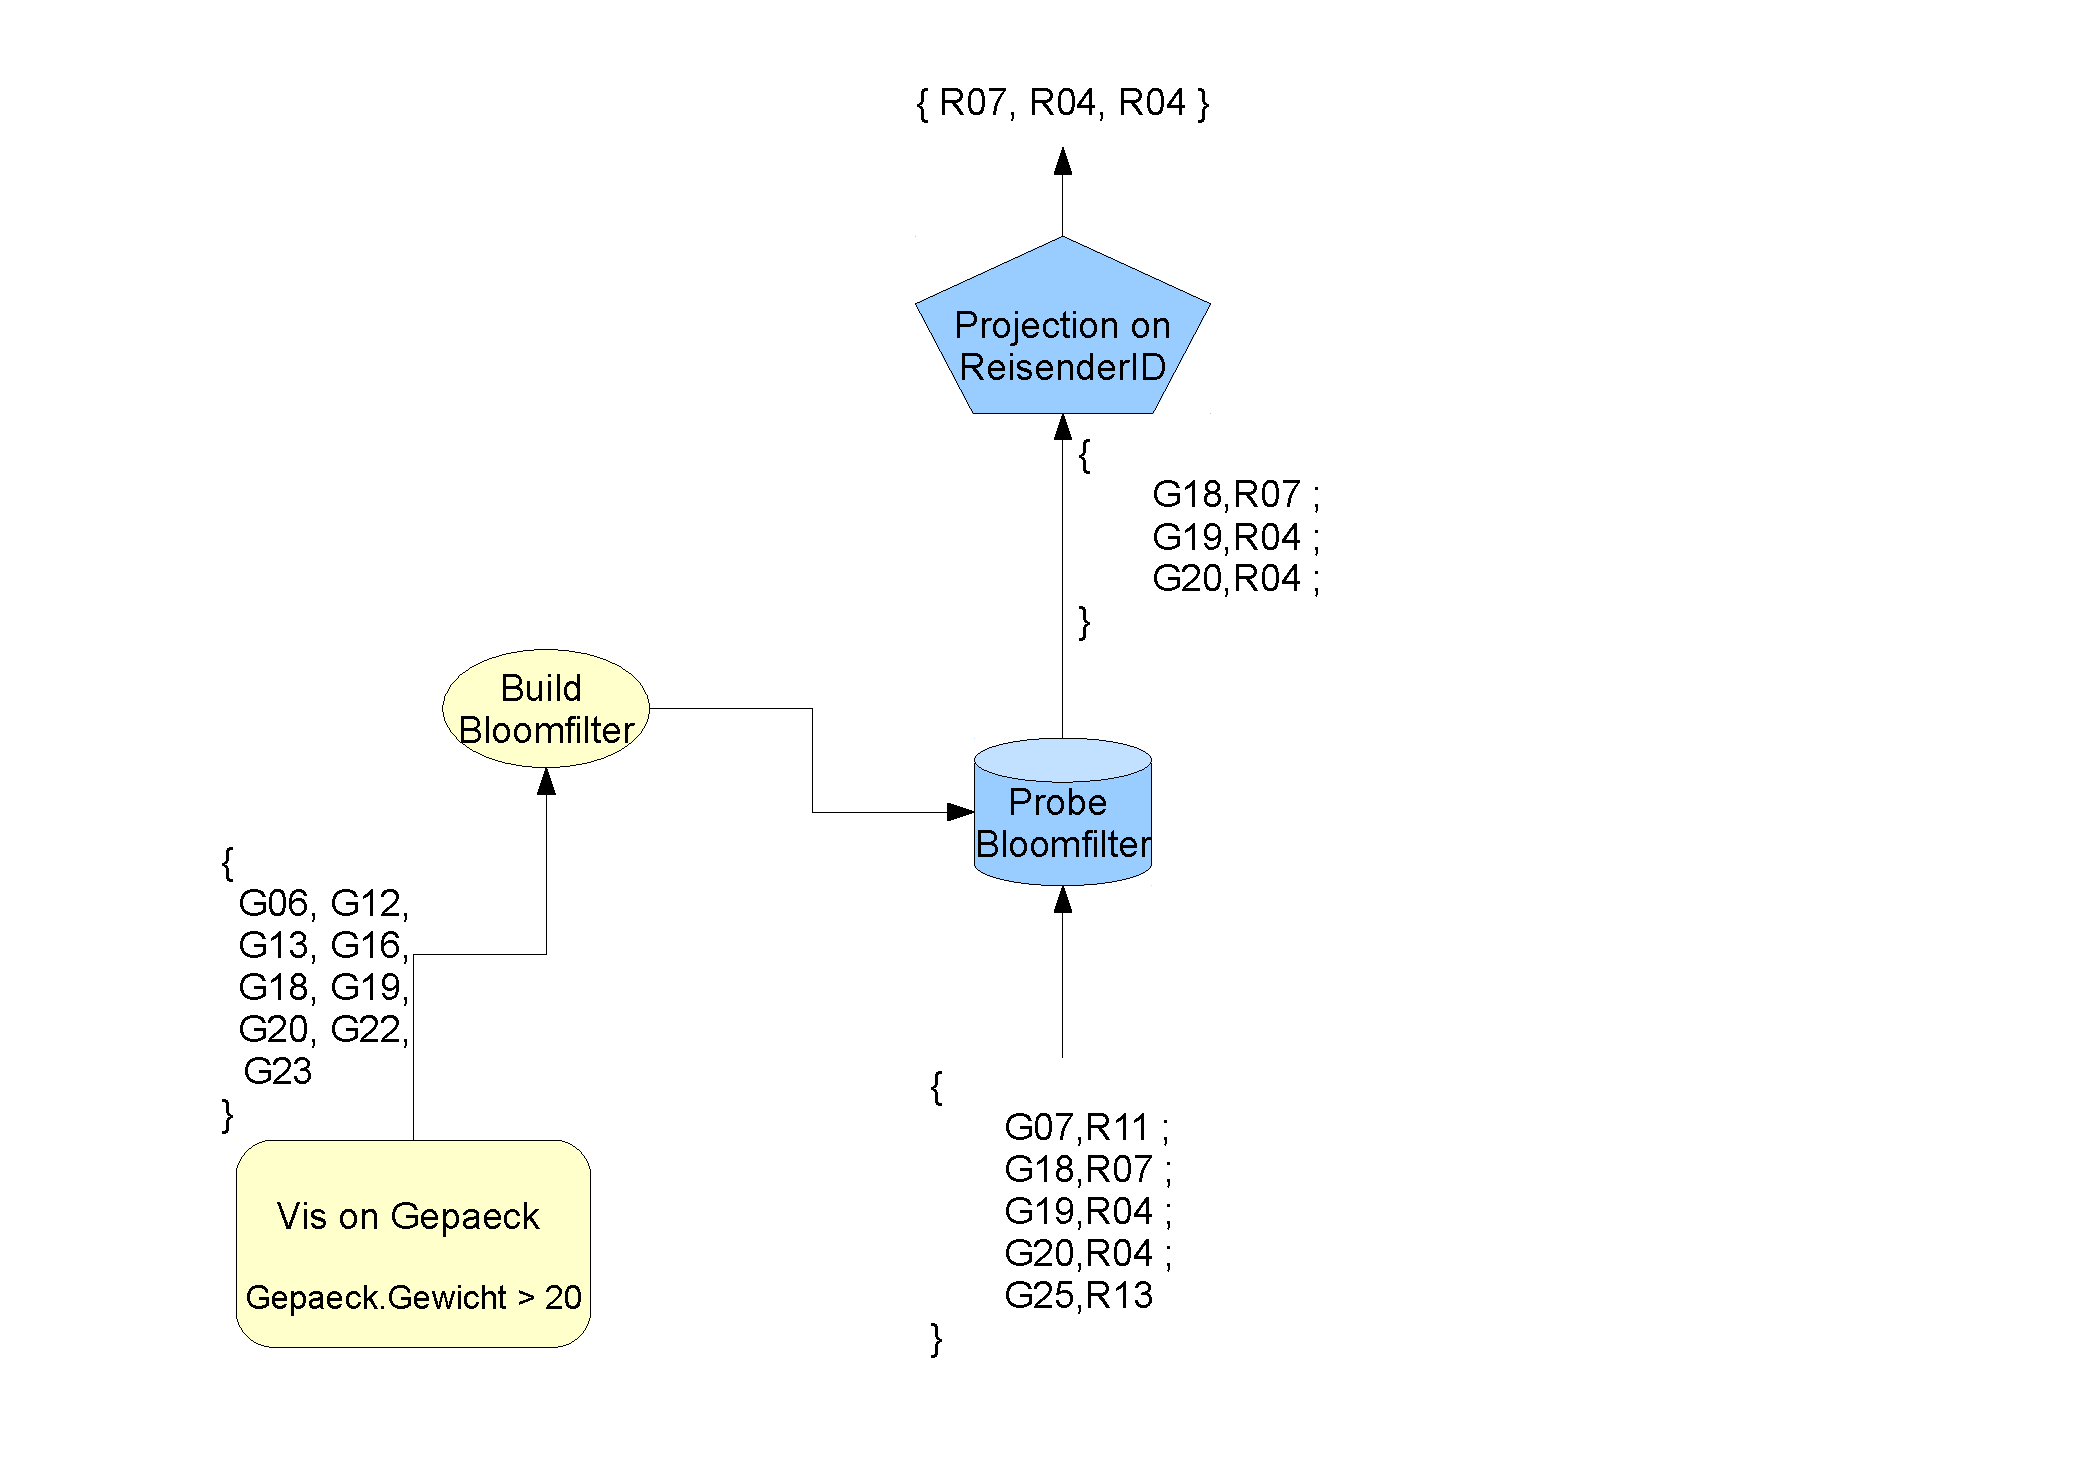
\includegraphics[trim = 0mm 10mm 0mm 10mm, clip, width=\textwidth]{img/Post3.pdf}
  \caption{Teilergebnis Postfiltering 3}
  \label{fig:post3}
\end{figure}

Mittels ``Climbing Index'' ist der Schritt von \textit{Pilot.Geburtsdatum} auf \textit{BuchungsID} m�glich: \{\{\}, \{B08, B11, B18, B19, B20, B21\}, \{\}, \{\}\}. Durch Verwendung von Merge und eines ``Subtree Key Tables'' wird eine Liste von \textit{ReisenderIDs} berechnet: \{R07, R03, R13, R05, R04, R11\}.

\begin{figure}[H]
  \centering
  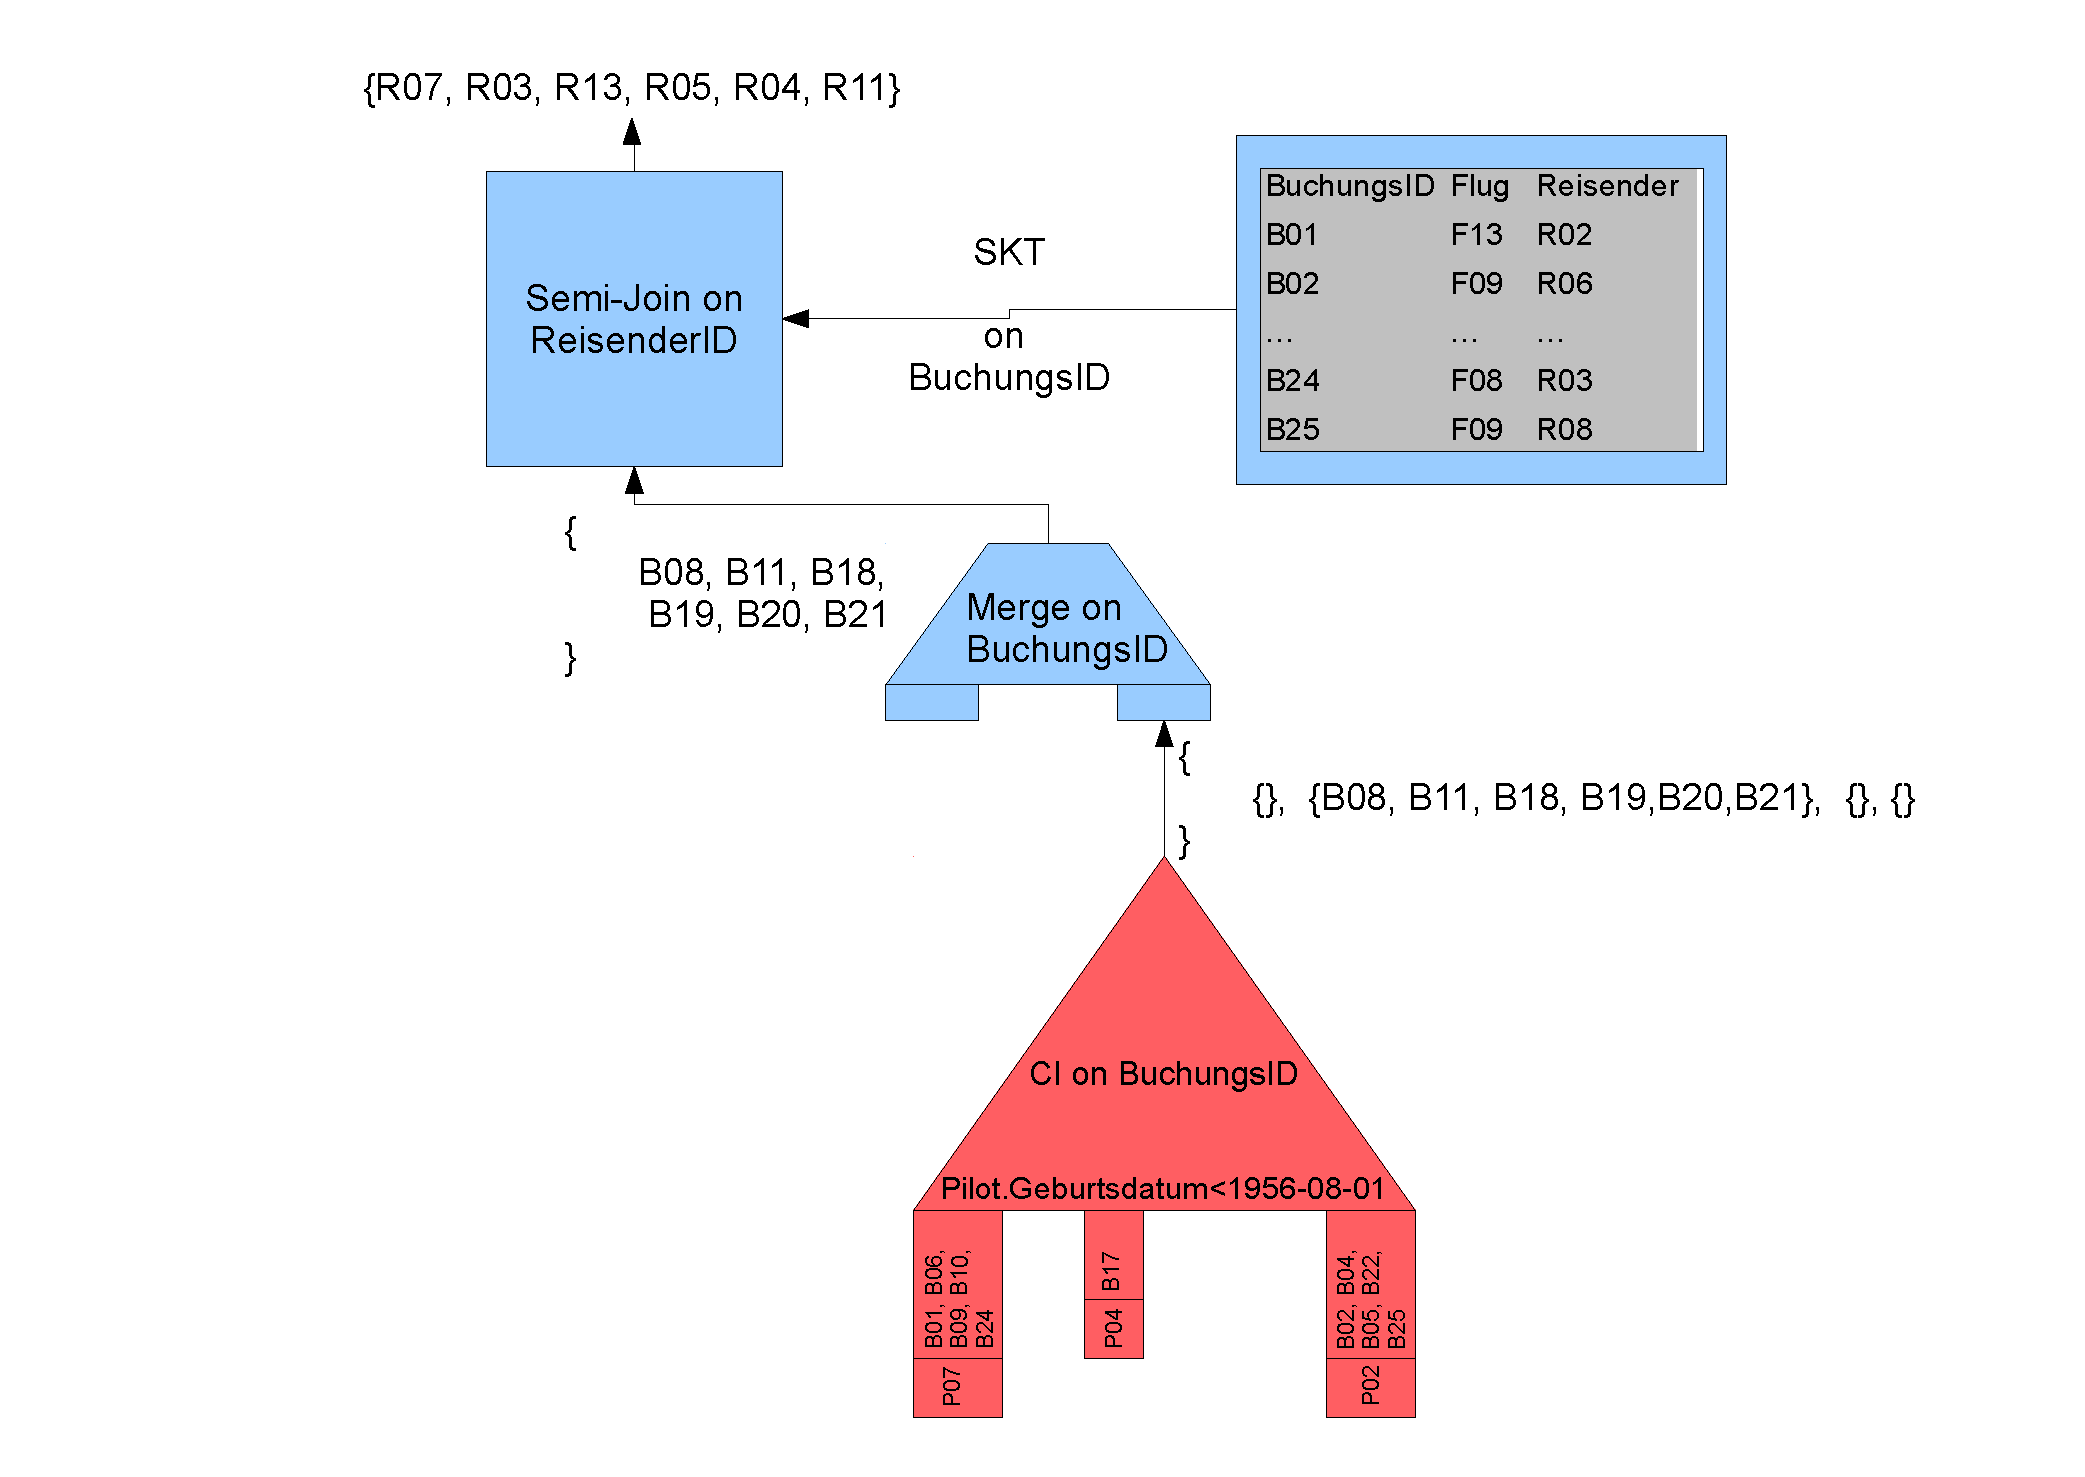
\includegraphics[trim = 0mm 10mm 0mm 0mm, clip, width=\textwidth]{img/Post4.pdf}
  \caption{Teilergebnis Postfiltering 4}
  \label{fig:post4}
\end{figure}

Aus dem Durchschnitt beider Listen von \textit{ReisenderIDs} wird ein Bloom-Filter erzeugt. Dieser wird auf das �bermittelte Zwischenergebnis des unsicheren Ger�ts, Reisender.Geschlecht='M', angewendet. Durch Verwendung des MJoin-Operators wird das Ergebnis erzeugt: \\\{$\langle$R04,Doru,Davidovici,Rom�nisch$\rangle$\}.

\begin{figure}[H]
  \centering
  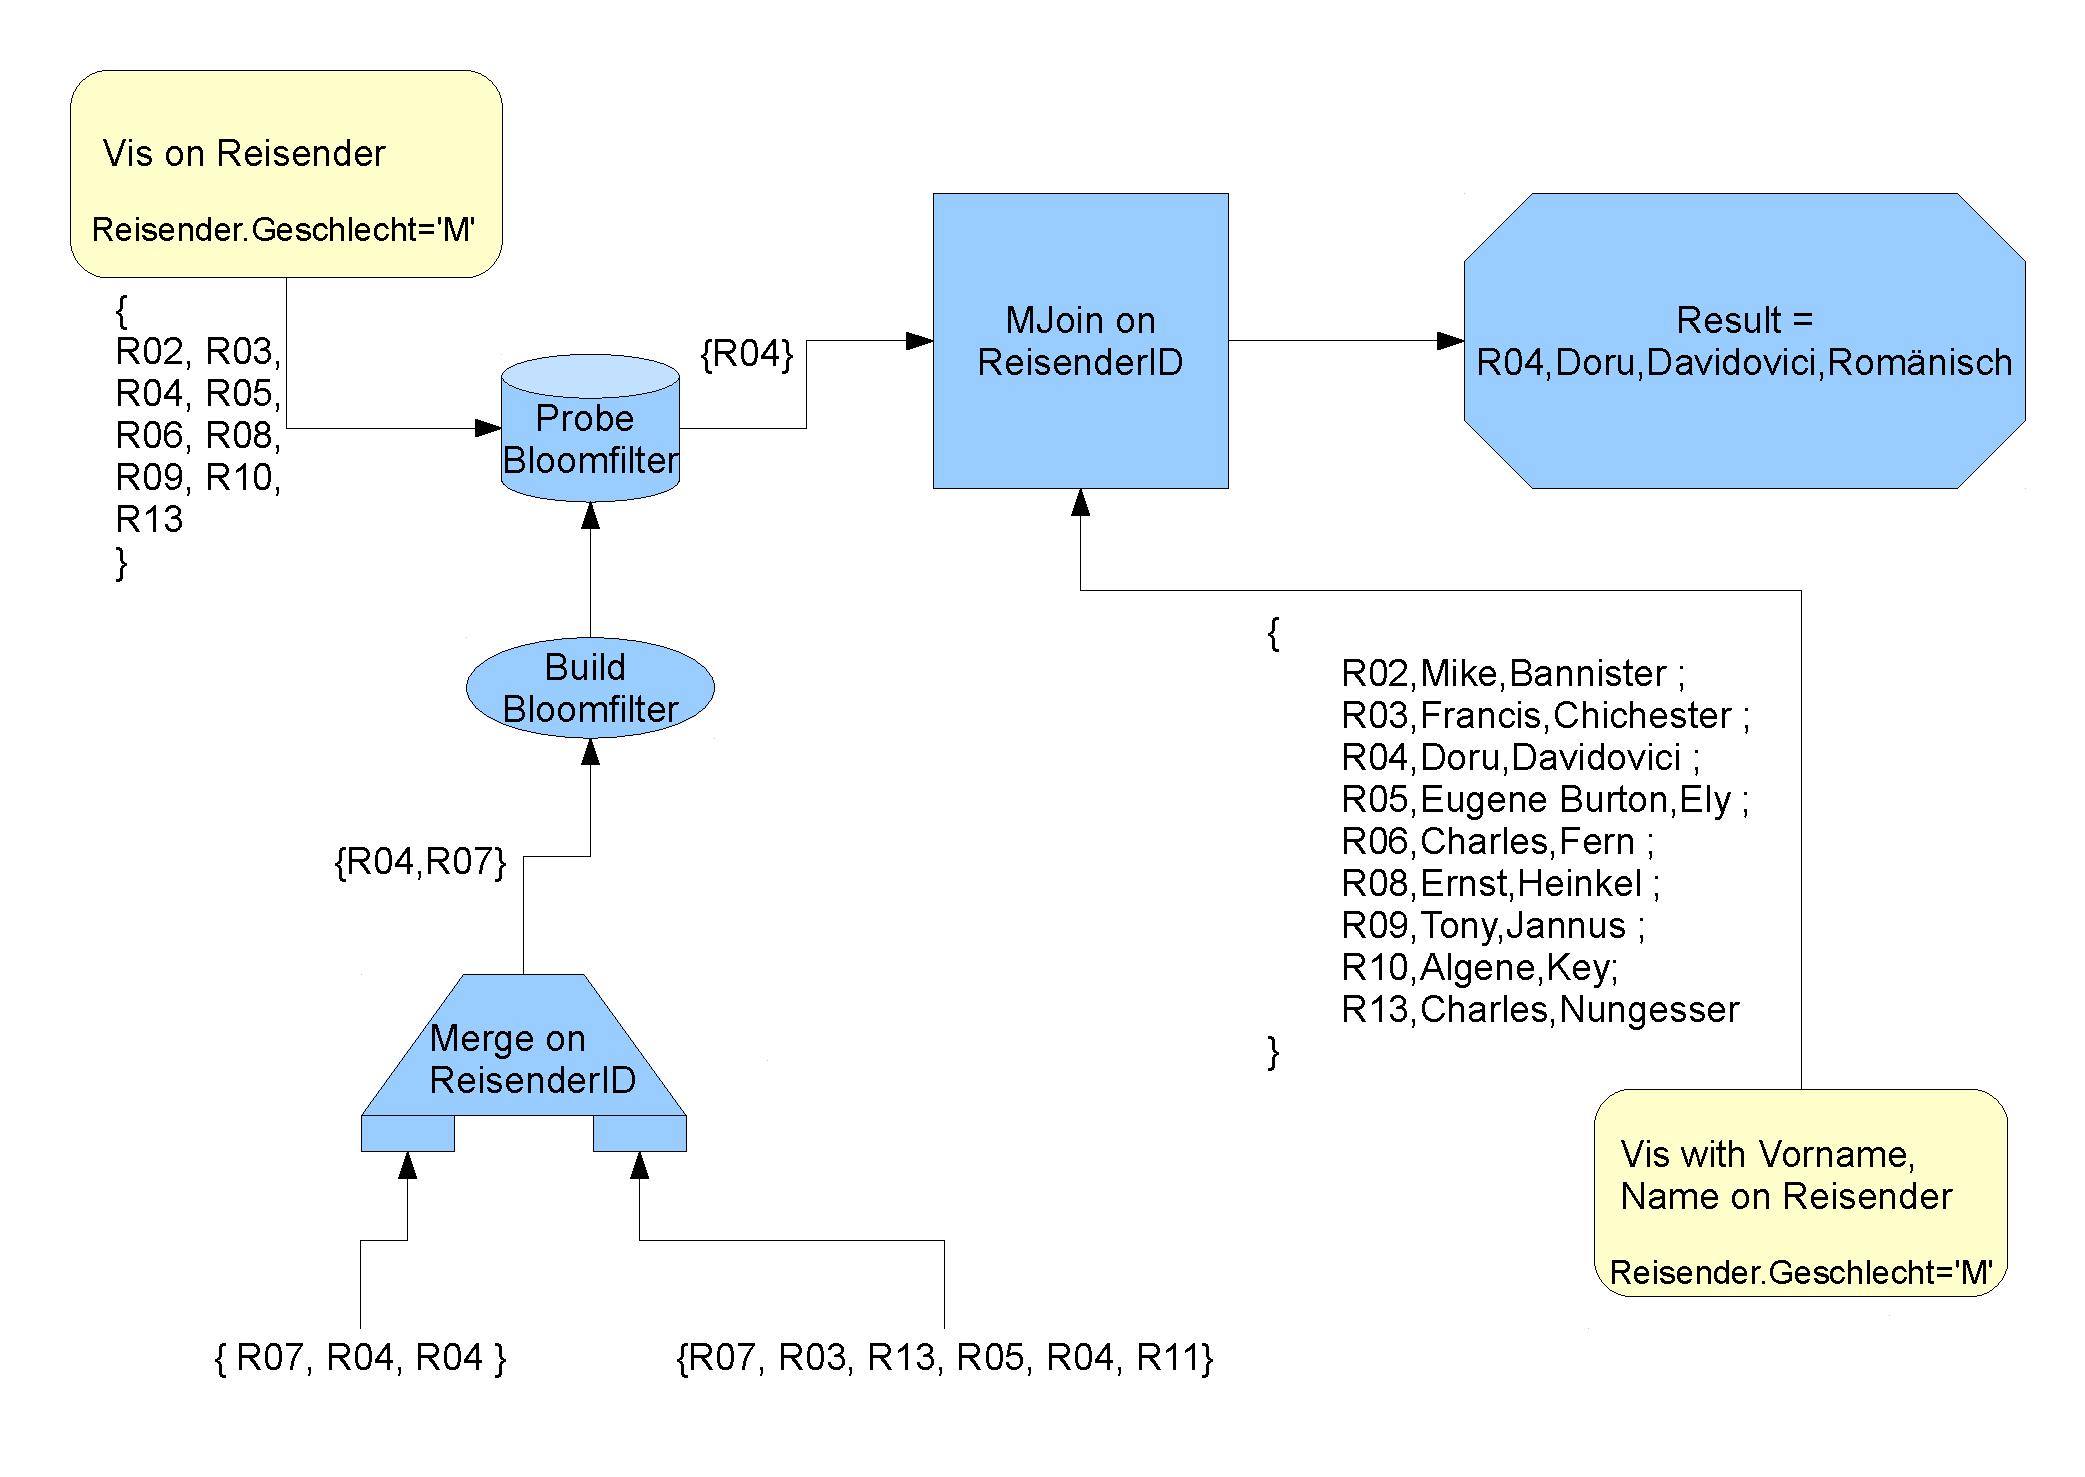
\includegraphics[trim = 0mm 10mm 0mm 0mm, clip, width=1\textwidth]{img/Post5.pdf}
  \caption{Teilergebnis Postfiltering 5}
  \label{fig:post5}
\end{figure}

F�gt man alle Teile zusammen, erh�lt man den kompletten Ablaufplan f�r unsere Anfrage:

\begin{figure}[H]
  \centering
  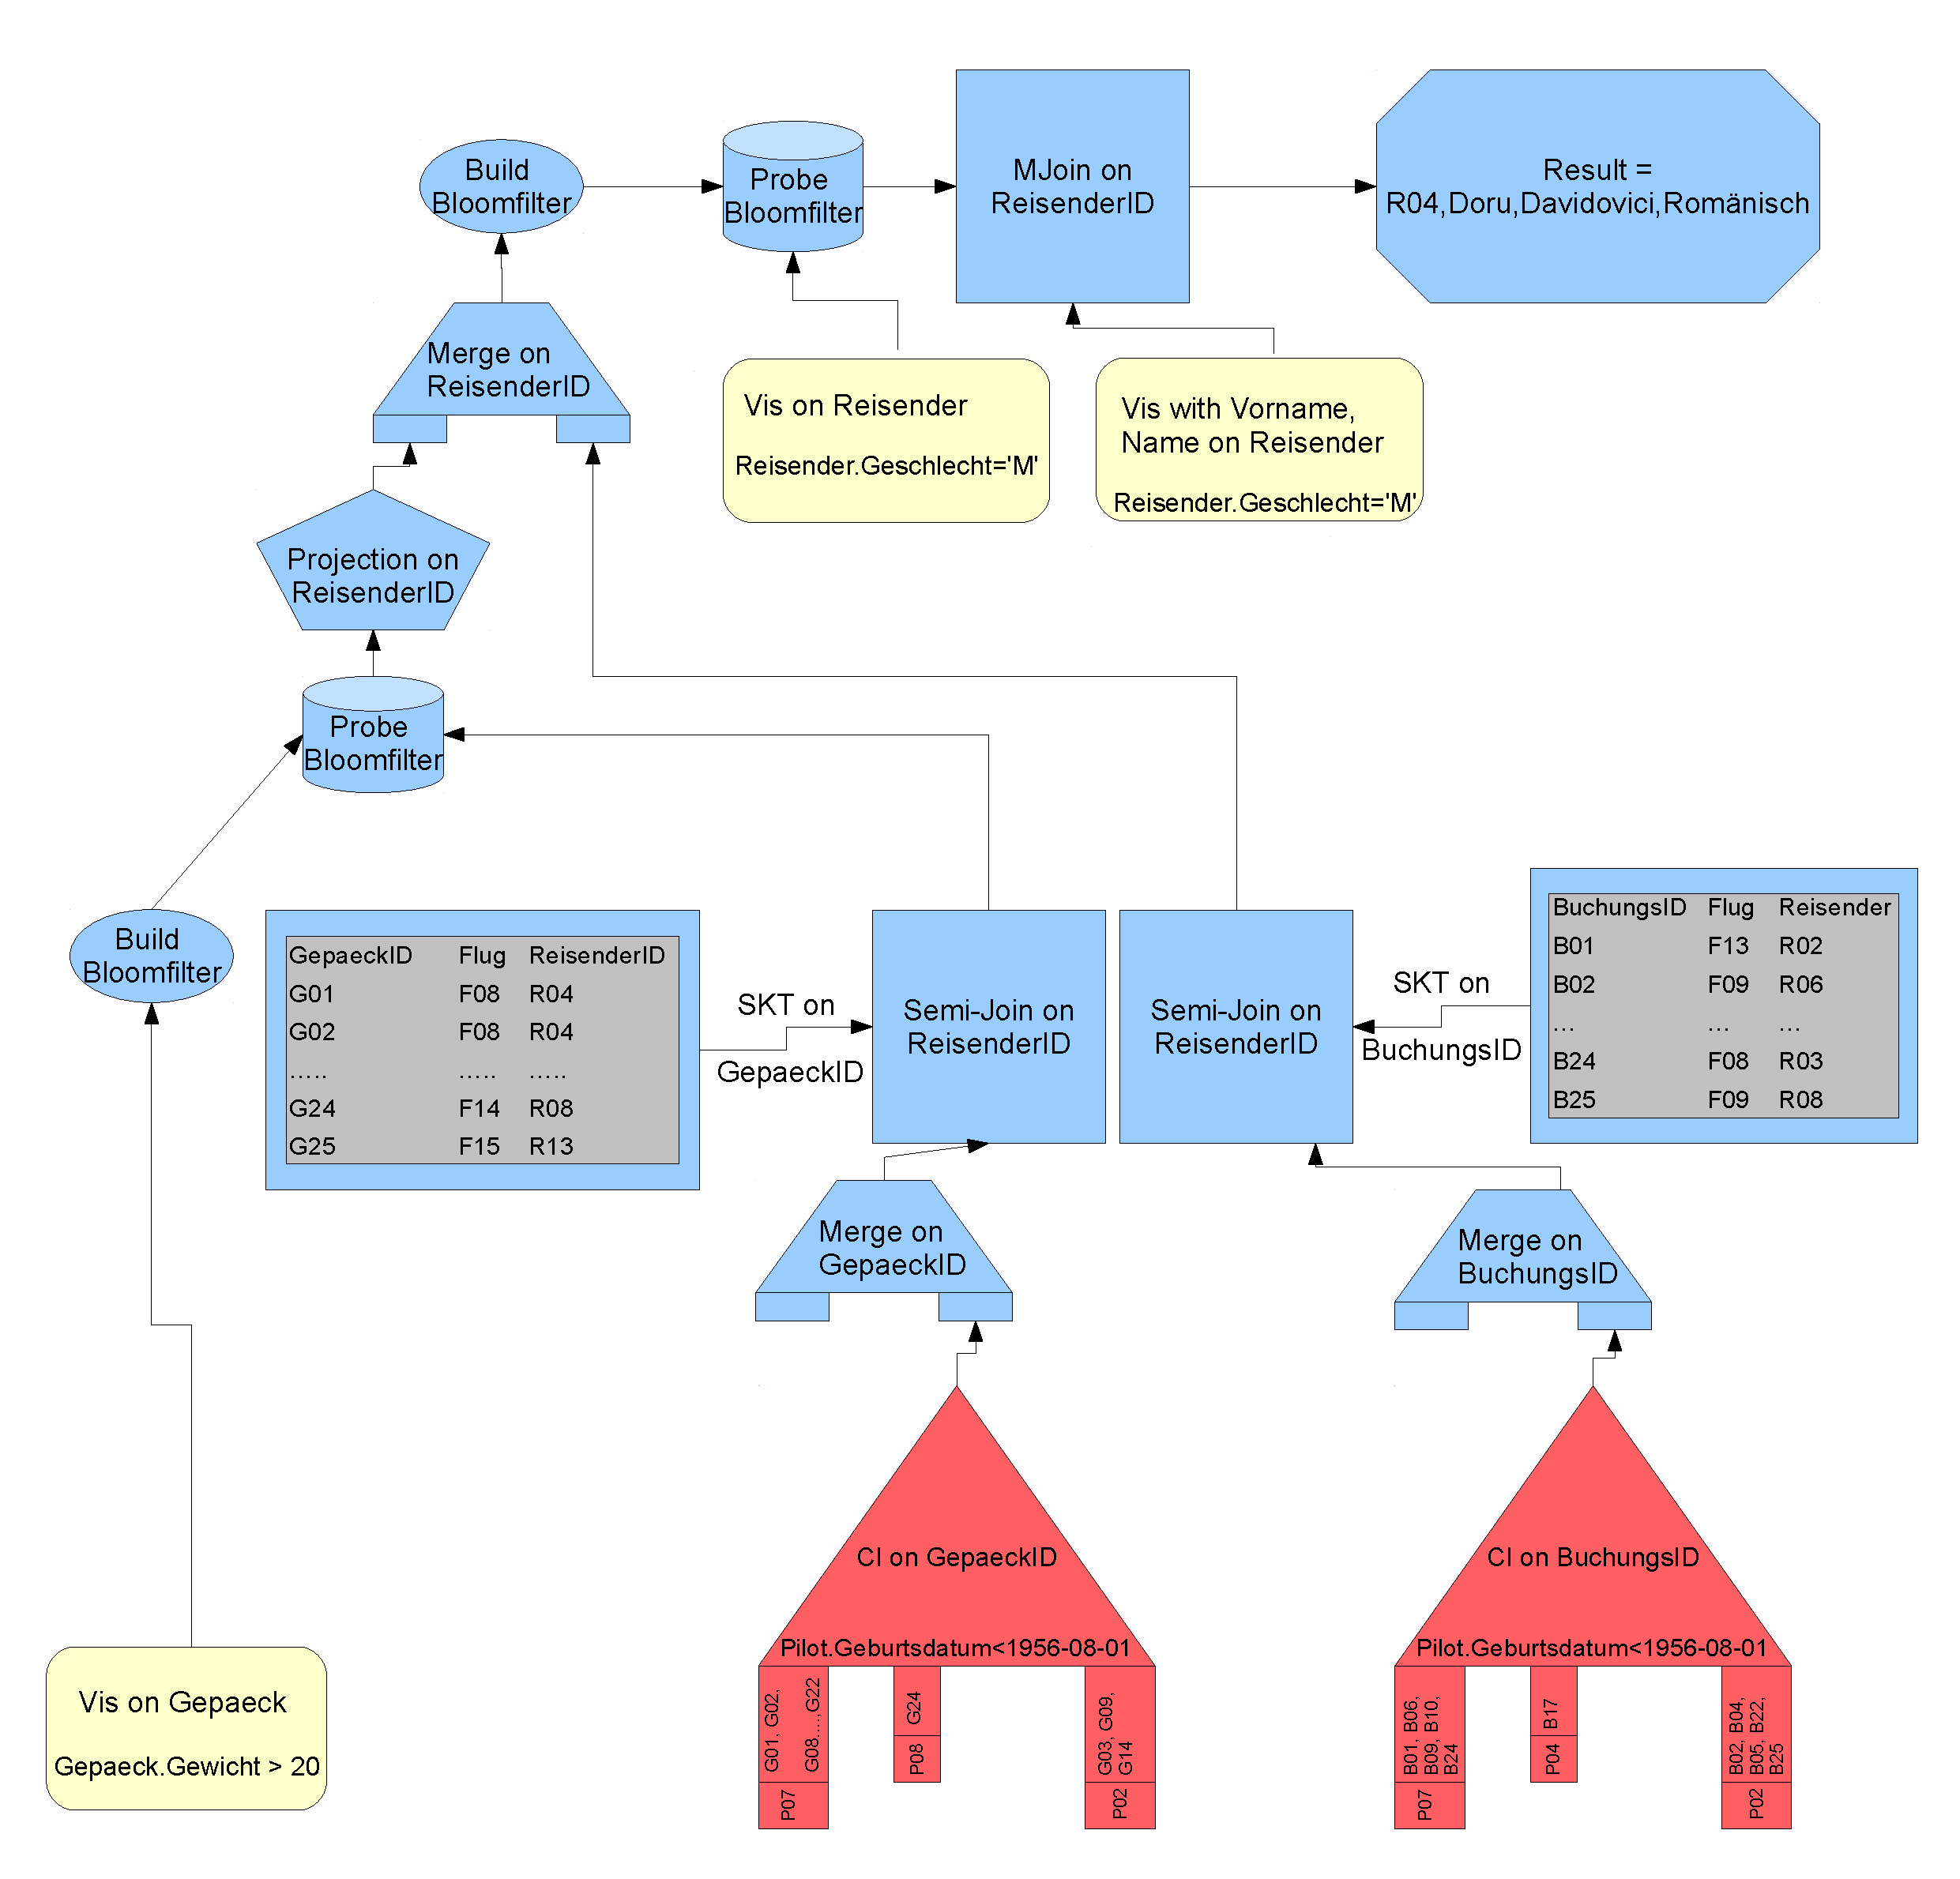
\includegraphics[trim = 0mm 10mm 0mm 0mm, clip, width=\textwidth]{img/Post-Filtering.pdf}
  \caption{Postfiltering QEP}
  \label{fig:post}
\end{figure}

Unter Verwendung der in \cite{ghostdb1} definierten Operanden, l�sst sich der ``Postfiltering'' Plan auch wie folgt aufschreiben:

\begin{enumerate}[1]
\item CI(P.Geburtsdatum,<1956-08-01,G.GepaeckID) = \{\{\}, \{G07, G18, G19, G20, G25\}, \{\}, \{\}\}
\item Merge($\bigcup 1$) = \{G07, G18, G19, G20, G25\}
\item SJoin(2,$\text{SKT}_{\text{Gepaeck}}$,$\langle$G.GepaeckID,R.ReisenderID$\rangle$) = \{$\langle$G07,R11$\rangle$, $\langle$G18,R07$\rangle$, $\langle$G19,R04$\rangle$, $\langle$G20,R04$\rangle$, $\langle$G25,R13$\rangle$\}
\item Vis(Q,Gepaeck,G.GepaeckID) = \{G06, G12, G13, G16, G18, G19, G20, G22, G23\}
\item BuildBF(4) = BF
\item ProbeBF(BF,3) = \{$\langle$G18,R07$\rangle$, $\langle$G19,R04$\rangle$, $\langle$G20,R04$\rangle$\}
\item Project(6,R.ReisenderID) = \{R07, R04, R04, R02, R01\}
\item CI(P.Geburtsdatum,<1956-08-01,B.BuchungsID) = \{\{\}, \{B08, B11, B18, B19, B20, B21\}, \{\}, \{\}\}
\item Merge($\bigcup 8$) = \{B08, B11, B18, B19, B20, B21\}
\item SJoin(9,$\text{SKT}_{\text{Buchungen}}$,R.ReisenderID) = \{R07, R03, R13, R05, R04, R11\}
\item Merge($7\cap 10$) = \{R04, R07\}
\item BuildBF(11) = BF
\item Vis(Q,Reisende,R.ReisenderID) = \{R02, R03, R04, R05, R06, R08, R09, R10, R13\}
\item ProbeBF(BF,13) = \{R04\}
\item Vis(Q,Reisende,$\langle$R.ReisenderID,R.Vorname,R.Name$\rangle$) = \{$\langle$R02,Mike,Bannister$\rangle$, \\$\langle$R03,Francis,Chichester$\rangle$, $\langle$R04,Doru,Davidovici$\rangle$, $\langle$R05,Eugene Burton,Ely$\rangle$, $\langle$R06,Charles,Fern$\rangle$, $\langle$R08,Ernst,Heinkel$\rangle$, $\langle$R09,Tony,Jannus$\rangle$, \\$\langle$R10,Algene,Key$\rangle$, \\$\langle$R13,Charles,Nungesser$\rangle$\}
\item MJoin(15,14,$\langle$R.ReisenderID,R.Staatsbuergerschaft$\rangle$,11) = \{$\langle$R04,Doru,Davidovici,Rom�nisch$\rangle$\}
\end{enumerate}

%
\end{document}
